\documentclass[review]{elsarticle}

\usepackage{amsmath}
\usepackage{booktabs}
\usepackage{dirtytalk}
\usepackage{subcaption}
\usepackage{tabularx}
%\usepackage{natbib}
\usepackage{nicefrac}
\usepackage[usenames]{xcolor}
\usepackage{lineno,hyperref}
\modulolinenumbers[5]

\journal{TBA}

%%%%%%%%%%%%%%%%%%%%%%%
%% Elsevier bibliography styles
%%%%%%%%%%%%%%%%%%%%%%%
%% To change the style, put a % in front of the second line of the current style and
%% remove the % from the second line of the style you would like to use.
%%%%%%%%%%%%%%%%%%%%%%%

%% Numbered
%\bibliographystyle{model1-num-names}

%% Numbered without titles
%\bibliographystyle{model1a-num-names}

%% Harvard
%\bibliographystyle{model2-names.bst}\biboptions{authoryear}

%% Vancouver numbered
%\usepackage{numcompress}\bibliographystyle{model3-num-names}

%% Vancouver name/year
%\usepackage{numcompress}\bibliographystyle{model4-names}\biboptions{authoryear}

%% APA style
%\bibliographystyle{model5-names}\biboptions{authoryear}

%% AMA style
%\usepackage{numcompress}\bibliographystyle{model6-num-names}

%% `Elsevier LaTeX' style
\bibliographystyle{elsarticle-num}
%%%%%%%%%%%%%%%%%%%%%%%

\begin{document}

\begin{frontmatter}

\title{Energy release rate of the fiber/matrix interface crack in UD composites under transverse loading: debond-debond and debond-free boundary interactions}
%\tnotetext[mytitlenote]{Fully documented templates are available in the elsarticle package on \href{http://www.ctan.org/tex-archive/macros/latex/contrib/elsarticle}{CTAN}.}

%% Group authors per affiliation:
%\author{Luca Di Stasio\fnref{myfootnote}}
%\address{Radarweg 29, Amsterdam}
%\fntext[myfootnote]{Since 1880.}

%% or include affiliations in footnotes:
\author[nancy,lulea]{Luca Di Stasio}
\author[lulea]{Janis Varna}
\author[nancy]{Zoubir Ayadi}
%\ead[url]{www.elsevier.com}

%\author[mysecondaryaddress]{Global Customer Service\corref{mycorrespondingauthor}}
%\cortext[mycorrespondingauthor]{Corresponding author}
%\ead{support@elsevier.com}

\address[nancy]{Universit\'e de Lorraine, EEIGM, IJL, 6 Rue Bastien Lepage, F-54010 Nancy, France}
\address[lulea]{Lule\aa\ University of Technology, University Campus, SE-97187 Lule\aa, Sweden}

\begin{abstract}
\noindent
%\textcolor{purple}{{\em Priority}: 1}\\
%\textcolor{purple}{{\em Target journal(s)}: Composites Part B: Engineering, Composites Part A: Applied Science and Manufacturing, Composite Structures, Journal of Composite Materials, Composite Communications}\\
The effects of crack shielding, finite thickness of the composite and fiber content on fiber/matrix debond growth in thin unidirectional composites are investigated analyzing  Representative Volume Elements (RVEs) of different ordered microstructures. Debond growth is characterized by estimation of the Energy Release Rates (ERRs) in Mode I and Mode II using the Virtual Crack Closure Technique (VCCT) and the J-integral. It is found that increasing fiber content, larger distance between debonds in the loading direction and the presence of a free surface close to the debond have all a strong enhancing effect on the ERR. The presence of fully bonded fibers in the composite thickness direction has instead a constraining effect, and it is shown to be very localized. An explanation of these observations is proposed based on mechanical considerations.
\end{abstract}

\begin{keyword}
Polymer-matrix Composites (PMCs)\sep Thin-ply\sep Transverse Failure \sep Debonding \sep Finite Element Analysis (FEA)
\end{keyword}

\end{frontmatter}

\linenumbers

\section{Introduction}

Stimulated by the ever more stringent requirements in terms of weight and mechanical performances of the aerospace industry, in recent years the composite community has returned its attention to the mechanisms of intralaminar crack initiation in general and to initiation of multiple cracking in thin-ply laminates in particular. Alternative design approaches are now considered based on this non-conventional laminate in applications ranging from cryogenic pressure vessels~\cite{McCarville2018}, to airplanes' wings~\cite{Kim2017}, and even reusable space launchers~\cite{Kopp2017}.\\
\emph{Thin-ply} laminates are the result of a technological innovation, the \emph{spread tow technology}, which consists in opening or spreading the tows in which fibers (carbon, glass, aramid, basalt among others) are usually shipped in into very thin tapes then used for laminate production. Ply thicknesses of less than $50\ \mu m$ can nowadays be mass-produced, and record thicknesses of around $20-25\ \mu m$, or $\sim 4-5$ times the average fiber's diameter, have been achieved. The technique in its current form, sometimes referred to as \say{FUKUI method} from the name of the Japanese prefecture it originated in, was firstly proposed towards the end of the 1990s~\cite{Kawabe1997} and perfected in the subsequent decade~\cite{Kawabe2008,Kawabe2008en}.\\
Several experimental investigations on \emph{thin ply} laminates have highlighted their main properties~\cite{Sasayama2003,Tsai2005,Yamaguchi2005,Sihn2007,Yokozeki2008,Yokozeki2010,Moon2011,Arteiro2013,Arteiro2014,Amacher2014,Guillamet2014,Huang2018,Cugnoni2018}: increased fiber content; more uniform packing of fibers; delay and even suppression of intralaminar cracking (called also transverse-, matrix- or micro-cracking) and delamination. A very insightful work documenting how these mechanisms are affected by the morphology of \emph{thin ply} laminates is the microscopic study of Saito \& al.~\cite{Saito2012}, which focuses on the effect of ply thickness on the onset and propagation of intralaminar cracking. In their investigation, tensile tests were performed on carbon fiber/epoxy $\left[0_{2},90_{n},0_{2}\right]$ \emph{thin-ply} laminates for $n=1,2,4$ and the crack density was measured at several levels of applied tensile strain in the range between $0\%$ and $1.5\%$. Furthermore, they performed microscopic observations on the specimen's edge at each level of strain. They observed the onset of fiber/matrix interface cracks (referred to as debonds in the following) at lower levels of strain in thinner plies, while at the same time coalescence of debonds and through-the-thickness propagation of transverse cracks in thin plies were delayed and even suppressed as ply thickness decreased. In particular, they reported the first onset of debonds at $0.4\%$ for $n=1,2$ and $0.7\%$ for $n=4$. For $n=1$, however, at $\varepsilon=1.5\%$ coalescence of debonds had started to take place but the crack had not completely propagated through the thickness, while for $n=2$ and $n=4$ the latter alreay happened at a value of strain respectively of $1.3\%$ and $1\%$. Our inability to explain these observations with the currently accumulated knowledge demonstrates the necessity of further investigation of interactions between debonds and studies of the constraining (or accelerating) effect of presence of bonded fibers, free and constrained boundaries in the vicinity of a partially debonded fiber.\\
Early studies on the effect of ply thickness on the onset and propagation of transverse cracks were conducted on glass fiber/epoxy cross-ply laminates by Bailey, Parvizi and collaborators~\cite{Garrett1977,Parvizi1978a,Parvizi1978b}, who firstly observed the beneficial effect of thickness reduction on the delay of transverse cracking. They furthermore pointed the attention to the appearance of debonds at the fiber/matrix interface and their subsequent coalescence as the mechanism at the origin of transverse cracks~\cite{Bailey1981}. Moreover, they identified the main mechanical driver of the damage process in the mismatch of elastic properties, and particularly of Poisson's ratios, between fibers and matrix~\cite{Bailey1979}. A full understanding of damage onset and propagation in \emph{thin-ply} laminates thus requires the comprehension of the mechanisms governing its very first stage, i.e. the fiber/matrix interface crack. First results were obtained through analytical models in the case of a single fiber with an arc crack (debond) in an infinite matrix under transverse tension by England~\cite{England1966} and Perlman \& Sih~\cite{Perlman1967}, who obtained the stresses at the interface and calculated the stress intensity factors at the crack tip, and by Toya~\cite{Toya1974}, who evaluated the Energy Release Rate (ERR). Drawing upon the results for the straight bi-material interface crack by Comninou~\cite{Comninou1977}, the effect of crack face contact in fiber-matrix debonding was investigated in~\cite{Paris1996,Varna1997a}. In~\cite{Garcia2015}, it was showed in terms of ERR why the case of a single asymmetric debond is more likely to be observed under remote transverse tension than two symmetric debonds on the same fiber. The effect of different types and combinations of loads on debonding have been studied for the single fiber model: compression~\cite{Correa2007}, residual thermal stresses~\cite{Correa2011}, biaxial tension-tension and tension-compression~\cite{Correa2013}, biaxial compression-compression and compression-tension~\cite{Correa2014}. The effect of the presence of nearby bonded fibers on the debonding of a fiber embedded in an infinite matrix has been studied under uniaxial transverse tension~\cite{Sandino2016}, biaxial tension~\cite{Sandino2016b} and uniaxial transverse compression~\cite{Sandino2018}. The effect of inter-fiber distance on debond growth has been studied for a partially debonded fiber at the center of a hexagonal cluster inside a homogenized UD composite in the case of fully bonded neighbouring fibers~\cite{Zhuang2018} and of two partially debonded fibers out of the surrounding six~\cite{Varna2017}. An understanding of crack shielding and finite thickness effects on debond growth in non-homogenized microstructural models of UDs seems thus to be lacking: this is the problem that we want to address in the present work. Mode I and Mode II energy release rates will be analyzed using stress fields calculated with the FEM for a variety of Repeating Unit Cell (RUC) of the composite with square packing of fibers under transverse tensile loading. These RUCs represent composites with different distance between partially debonded fibers in the transverse direction which allows to study the effect of crack shielding on the ERR. In the ply thickness direction, the varying number of perfectly bonded fiber rows exposes the effect of the free boundary of the composite on debond growth. Finally, using coupling of thickness direction displacements on horizontal boundaries of the RUC, the accelerating effect of the interaction between debonds of fibers located on the same vertical line is studied.

%%%%%%%%%%%%%%%%%%%%%%%%%%%%%%%%%%%%%%%%%%%%%%%%%%%%%%%%%%%%%%%%%%%
%%%%%%%%%%%%%%%%%%%%%%%%%%%%%%%%%%%%%%%%%%%%%%%%%%%%%%%%%%%%%%%%%%%
\section{RVE models \& FE discretization}

\subsection{Introduction \& Nomenclature}\label{subsec:names}

In this paper, we analyze debond development in unidirectional (UD) composites subjected to in-plane transverse tensile loading.  The interaction between debonds in UD composites is studied developing models of different Repeating Unit Cells (RUC) of laminates where only the central fiber in the cell has a damage in the form of a fiber/matrix interface crack (debond). The composite RUC may be repeating in the in-plane transverse direction only (representing an ultra-thin composite) or repeating also in the composite thickness direction, representing an infinite composite in a limiting case. Thus, the conditions at the UD composite's upper and lower boundaries are one of the parameters for the investigation.  The used RUCs allow for considering the composite with debonds as a sequence of stacked damaged and undamaged rows, each row with only one fiber in the thickness direction. Since all of these RUCs feature regular microstructures with fibers placed according to a square-packing configuration, they are Representative Volume Elements (RVE) of composites with a certain distribution of debonds. Introducing in-plane coordinates x and y, where x is in the transverse direction of the UD composite under consideration, the strain in the y-direction due to a load in the x-direction is small, caused in turn by the very small minor Poisson's ratio of the UD composite. Additionally, debonds are considered to be significantly longer in the fiber direction than in the arc direction. Therefore, we use 2D models under the assumption of plane strain, defined in the $x-z$ section of the composite.  Thus, the analysis presented applies to long debonds, with a focus on understanding the mechanisms of growth along their arc direction. The composites are subjected to transverse tensile strain, applied as a constant displacement in the $x$-direction along the vertical boundary of the RUC as shown in  Figure~\ref{fig:laminateModelsA} to~\ref{fig:FEmodel}. As the models are differentiated by the number of rows of fibers and by the spacing between debonds along the vertical and horizontal directions, the corresponding RUCs can be distinguished from each other based on the number n of fibers in the horizontal direction and k in the vertical direction. Furthermore, the horizontal surfaces can be either free or vertical displacement coupling can be applied. We thus introduce the common notation$n\times k-free$  and $n\times k-coupling$ to denote a RUC with $n\times k$ fibers and, respectively, a free upper surface or kinematic coupling applied to it. The specific combinations of particular choices of $n$, $k$, and boundary conditions are detailed in Section~\ref{subsec:rve}, together with the description of the corresponding models of damaged composite they are representing.

\subsection{Models of Representative Volume Element (RVE)}\label{subsec:rve}

The first two models feature, as shown in Fig.~\ref{fig:laminateModelsA}, an ultra-thin UD laminate with only one row of fibers across its thickness, $k=1$. This is quite an extreme model from the microstructural point of view; however, it allows to focus the analysis on the interaction between debonded fibers placed along the x-direction. Furthermore, as the horizontal surfaces are considered free, the interaction is stronger in this case than in any other, making the trends very clear and the predictions of this model rather conservative. In retrospective, if only 20 years ago such a model would have been considered too abstracted from the physical reality, the recent advancements in the spread tow technology make this approach appealing also as a limiting case for practical considerations.

\begin{figure}[!h]
\centering
    \begin{subfigure}[b]{\textwidth}
        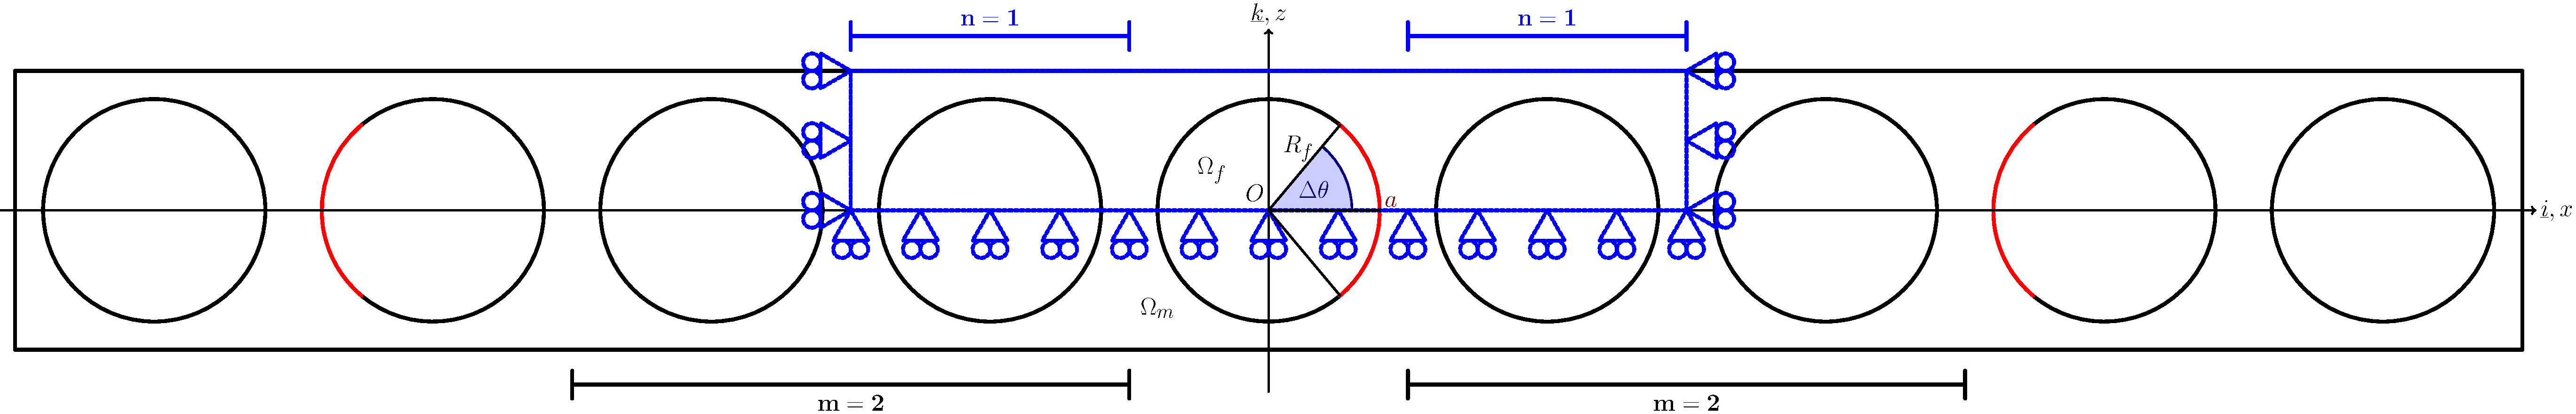
\includegraphics[width=\textwidth]{freeThinPly.pdf}
        \caption{Single row of fibers with a debond appearing every $n$ fibers: model $n\times1-free$ ($n=3$ in the figure).}\label{subfig:freethinply}
    \end{subfigure}

    \begin{subfigure}[b]{\textwidth}
        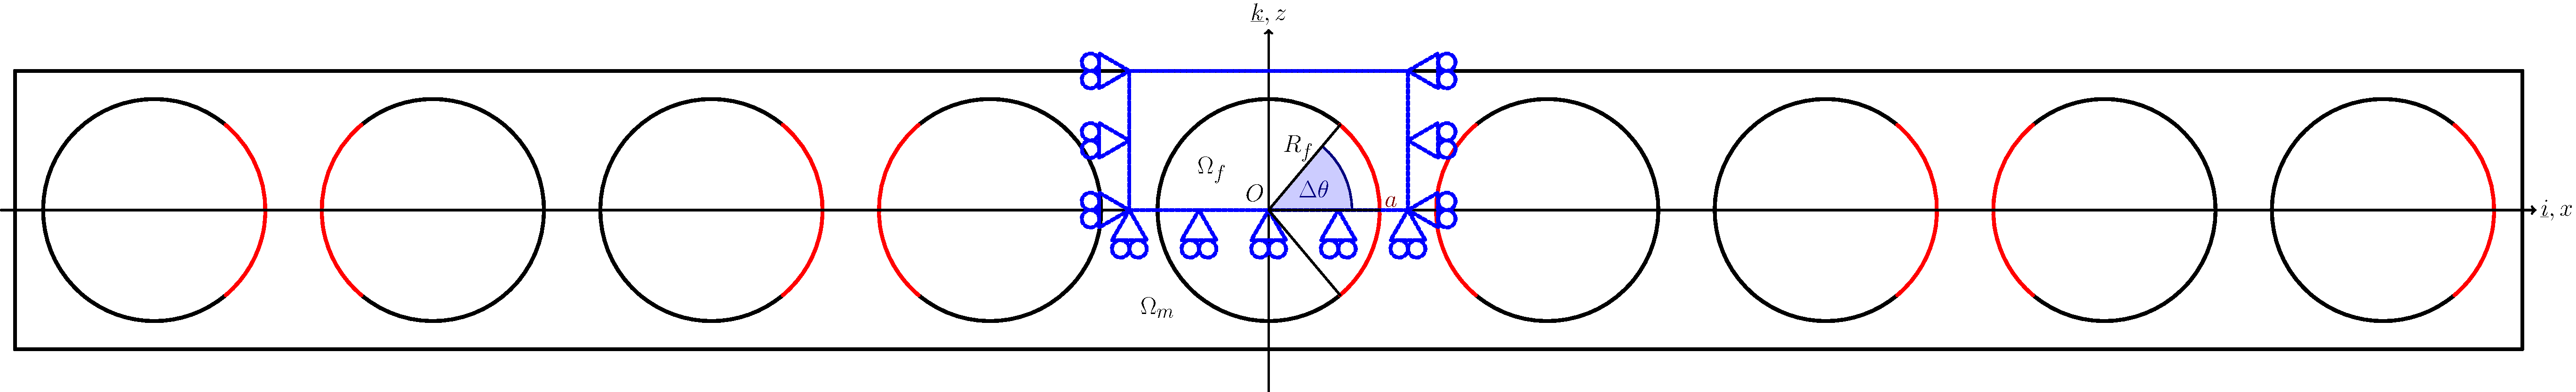
\includegraphics[width=\textwidth]{freeThinPlyAllDebonds.pdf}
        \caption{Single row of fibers with debonds appearing on each fiber: model $1\times1-free$ .}\label{subfig:freethinplyalldebonds}
    \end{subfigure}

\caption{Models of ultra-thin UD composites with a single ``row'' of fibers and debonds repeating at different distances. The corresponding repeating element (RUC) is highlighted in blue, while debonds are represented in red.}\label{fig:laminateModelsA}
\end{figure}

In the sub-model of Fig.~\ref{subfig:freethinply}, every $n^{th}$ fiber in the composite is partially debonded on alternating sides of the fiber. The symmetries of the model allow the use of the upper part of the RUC. It is highlighted by blue lines in Fig.~\ref{fig:laminateModelsA} to~\ref{fig:thickplyalldebonds}. Following the notation introduced in Section~\ref{subsec:names}, we will refer to this model as $n\times 1-free$. In the sub-model $n=1$, Fig.~\ref{subfig:freethinplyalldebonds}, a debond appears on each fiber on alternating sides and the corresponding RUC contains only one fiber. We will refer to this model as $1\times 1-free$.

\begin{figure}[!h]
\centering
    \begin{subfigure}[b]{\textwidth}
    \centering
        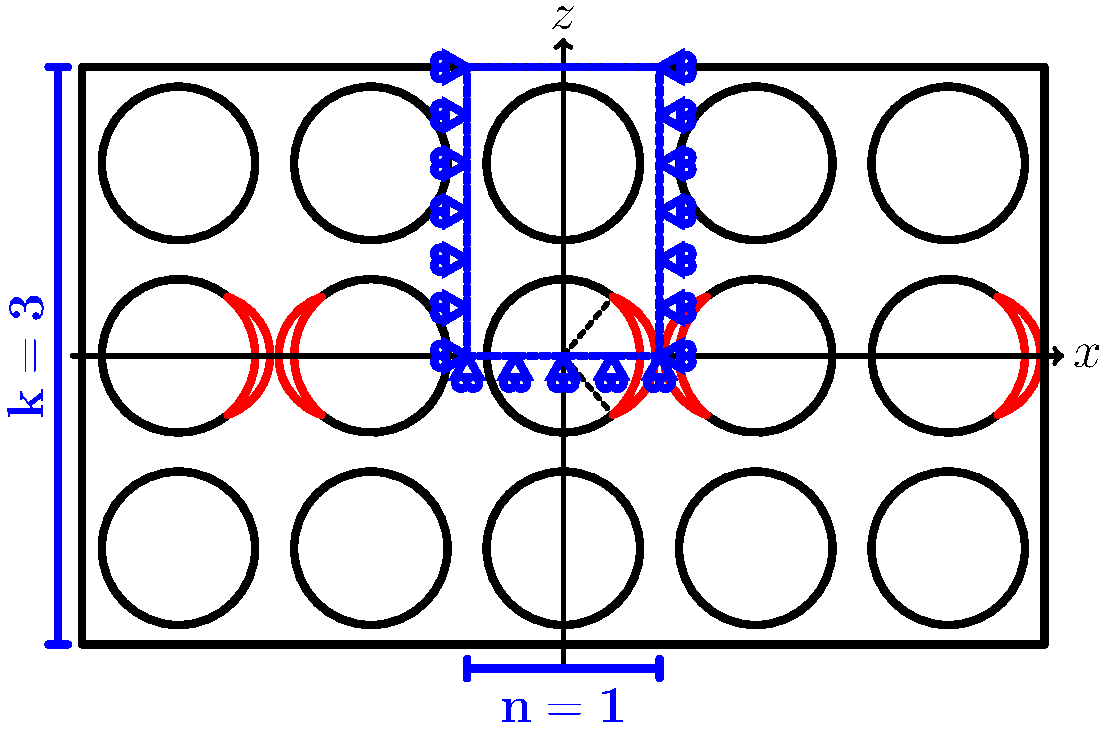
\includegraphics[height=0.3\textheight]{thickPlycentraldebondsline.pdf}
        \caption{Multiple rows of fibers with debonds appearing on each fiber beloging to the central row: model $1\times k-free$ ($k=3$ in the figure).}\label{subfig:thickplycentraldebonds}
    \end{subfigure}

    \begin{subfigure}[b]{\textwidth}
        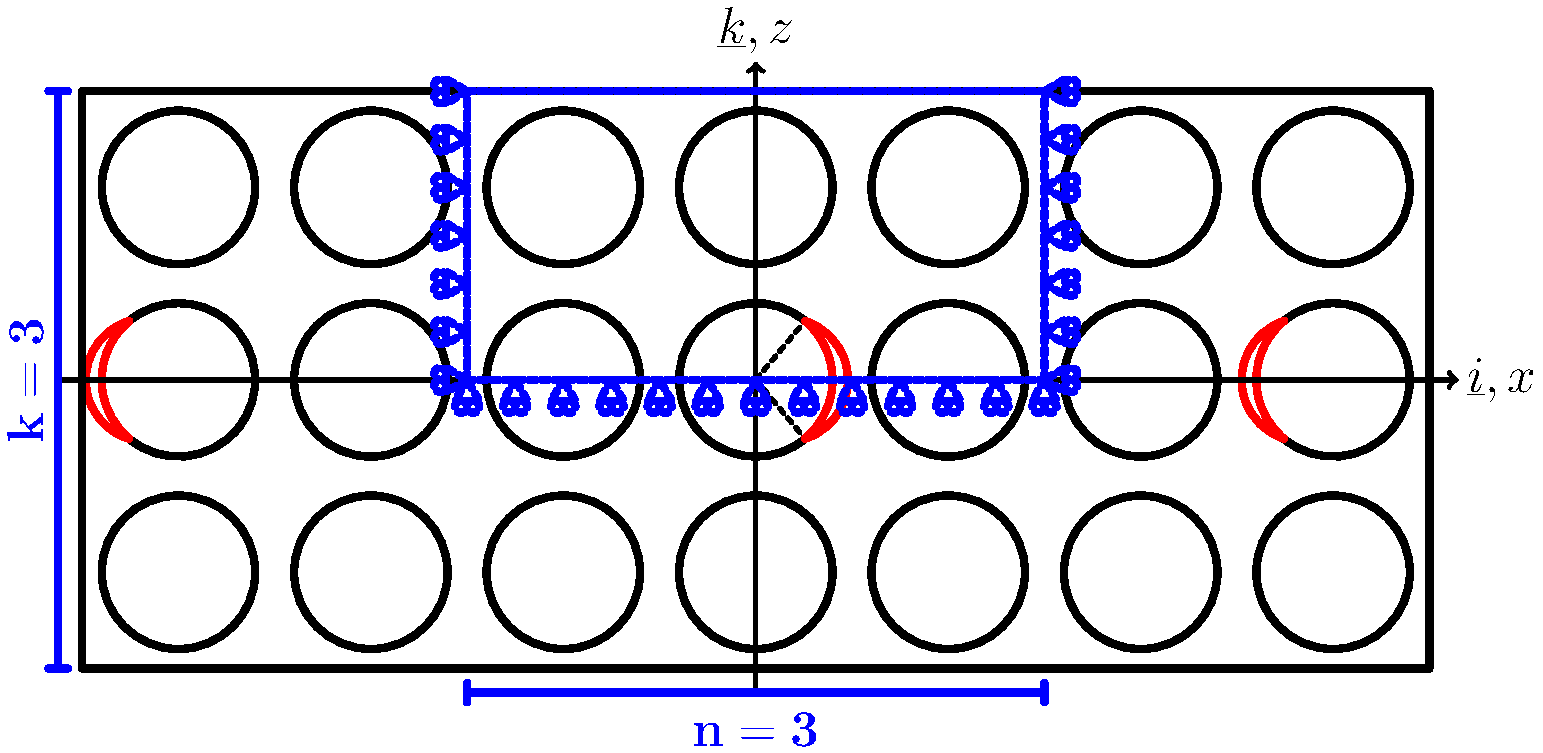
\includegraphics[width=\textwidth]{thickPly.pdf}
        \caption{Mutiple rows of fibers with a debond appearing every $n$ fibers within the central row: model $n\times k-free$ ($n=3$ and $k=3$ in the figure).}\label{subfig:thickply}
    \end{subfigure}

\caption{Models of UD composites with different ``rows'' of fibers and debonds repeating at different distances. The corresponding repeating element (RUC) is highlighted in blue, while debonds are represented in red.}\label{fig:laminateModelsB}
\end{figure}

The second set of models in Fig.~\ref{fig:laminateModelsB} and Fig.~\ref{fig:thickplyalldebonds} considers laminates with multiple rows of fibers across the thickness: a finite number of rows in the first two sub-models in Fig.~\ref{fig:laminateModelsB}; an infinite number in the model of Fig.~\ref{fig:thickplyalldebonds}. In Fig. ~\ref{subfig:thickplycentraldebonds}, the RUC contains $n=1$ fiber in the x-direction, $k$ fibers across the thickness and the central fiber is debonded. This model will be referred to in the following as $1\times k-free$. Thinking in terms of rows, in this model we have a central row where each fiber is debonded. This row is surrounded from each side by $\nicefrac{\left(k-1\right)}{2}$ rows with perfectly bonded fibers. In the sub-model in Fig.~\ref{subfig:thickply}, each $n^{th}$ fiber in the central row is debonded and this row is surrounded by $\nicefrac{\left(k-1\right)}{2}$ rows of undamaged fibers from each side. We will refer to this model as $n\times k-free$ (because the horizontal boundary of the RUC is free of any constraint).

\begin{figure}[!h]
\centering
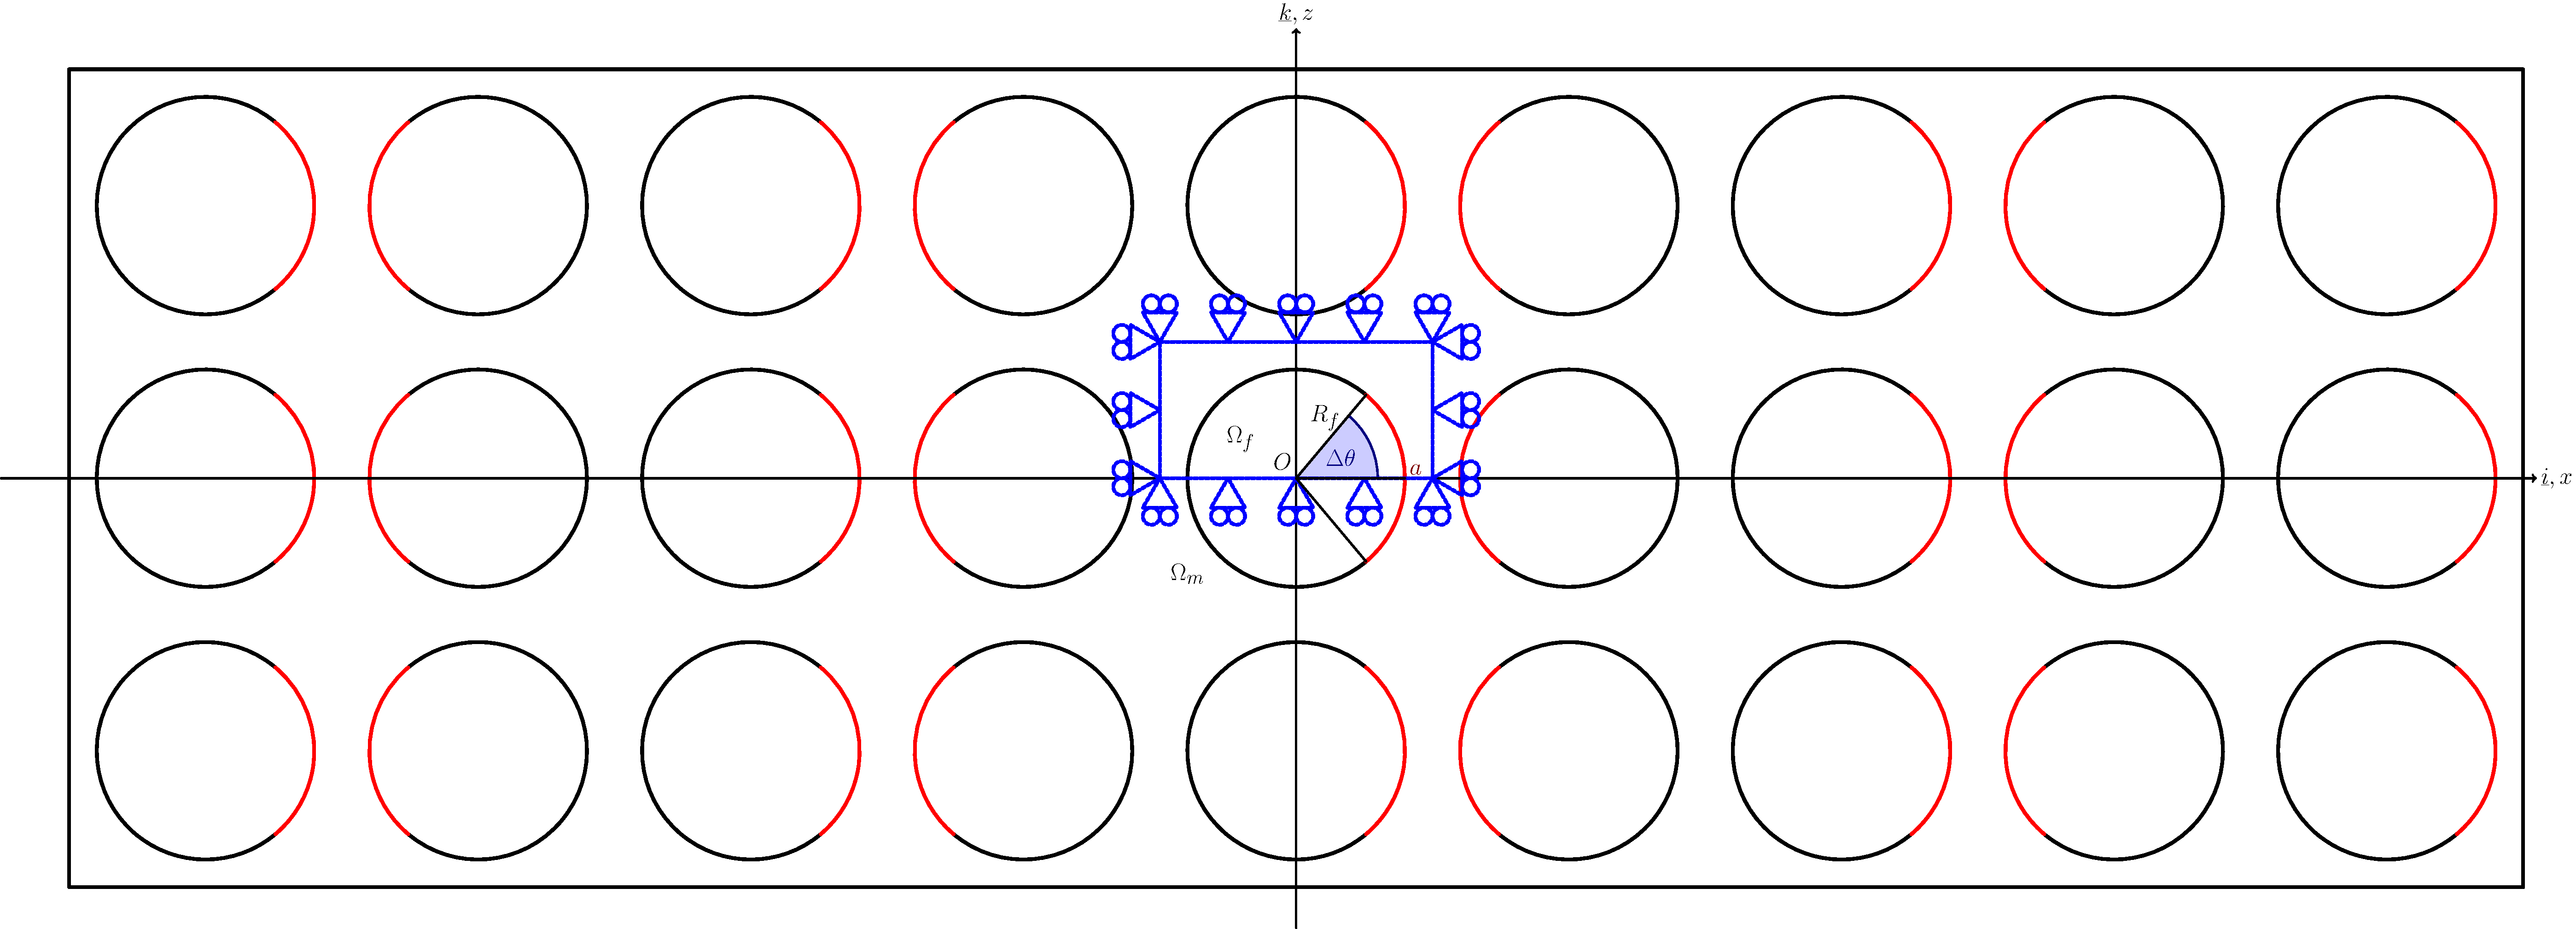
\includegraphics[width=\textwidth]{thickPlyAllDebonds.pdf}
\caption{Model of UD composites with an infinite number of  ``rows'' of fibers and debonds appearing on each fiber: model $1\times1-coupling$ . The corresponding repeating element (RUC) is highlighted in blue, while debonds are represented in red.}\label{fig:thickplyalldebonds}
\end{figure}

Finally, the model in Fig.~\ref{fig:thickplyalldebonds} represents an UD composite with an infinite number of rows; all of them with partially debonded fibers. As all fibers have debonds, the corresponding RUC is made of a single partially debonded fiber with kinematic coupling conditions applied to the upper boundary to assure periodicity. This model is referred to as $1\times 1-coupling$.

%\begin{table}[!h]
% \centering
% \caption{Summary of the models and their characteristics.}
% \begin{tabularx}{\textwidth}{p{0.05\textwidth}ccccc}
%\multicolumn{2}{c}{\textbf{Name}} & \multicolumn{4}{c}{\textbf{Boundary conditions}}\\
%                                                         &  & Up & Down & Right & Left \\
%\toprule
%\midrule
%\multicolumn{2}{c}{$\mathbf{D\left(m+1\right)H0V1L}$} &x-symmetry&free&coupling,&coupling,\\
%                                                         &  &  &  & $\bar{\varepsilon}_{x}=1\%$ & $\bar{\varepsilon}_{x}=1\%$ \\
%&\multicolumn{5}{X}{\small A debond every $\left(m+1\right)^{th}$ fiber in the horizontal direction, in a UD composites with 1 layer of fibers, Fig.~\ref{subfig:freethinply}.}\\
%\midrule
%\multicolumn{2}{c}{$\mathbf{D1H0V1L}$} &x-symmetry&free&coupling,&coupling,\\
%                                                         &  &  &  & $\bar{\varepsilon}_{x}=1\%$ & $\bar{\varepsilon}_{x}=1\%$ \\
%&\multicolumn{5}{X}{\small A debond every $1^{st}$ fiber in the horizontal direction, in a UD composites with 1 layer of fibers, Fig.~\ref{subfig:freethinplyalldebonds}.}\\
%\midrule
%\multicolumn{2}{c}{$\mathbf{D1H0V\left(2p+1\right)L}$} &x-symmetry&free&coupling,&coupling,\\
%                                                         &  &  &  & $\bar{\varepsilon}_{x}=1\%$ & $\bar{\varepsilon}_{x}=1\%$ \\
%&\multicolumn{5}{X}{\small A debond every $1^{st}$ fiber in the horizontal direction, in a UD composites with $\left(2p+1\right)$ layer of fibers, Fig.~\ref{subfig:thickplycentraldebonds}.}\\
%\midrule
%\multicolumn{2}{c}{$\mathbf{D\left(m+1\right)H0V\left(2p+1\right)L}$} &x-symmetry&free&coupling,&coupling,\\
%                                                         &  &  &  & $\bar{\varepsilon}_{x}=1\%$ & $\bar{\varepsilon}_{x}=1\%$ \\
%&\multicolumn{5}{X}{\small A debond every $\left(m+1\right)^{th}$ fiber in the horizontal direction, in a UD composites with $\left(2p+1\right)$ layers of fibers, Fig.~\ref{subfig:thickply}.}\\
%\midrule
%\multicolumn{2}{c}{$\mathbf{D1H1V\infty L}$} &x-symmetry&coupling&coupling,&coupling,\\
%                                                         &  &  &  & $\bar{\varepsilon}_{x}=1\%$ & $\bar{\varepsilon}_{x}=1\%$ \\
%&\multicolumn{5}{X}{\small A debond every $1^{st}$ fiber in the horizontal direction and every $1^{st}$ fiber in the vertical direction, in a UD composites with an infinite number of  layers of fibers, Fig.~\ref{fig:thickplyalldebonds}.}\\
%\bottomrule
%\end{tabularx}
%\label{tab:modelcharacteristics}
%\end{table}
%
%A summary of models' names and characteristics is reported in Table~\ref{tab:modelcharacteristics}

\subsection{Finite Element (FE) discretization}

Each RUC is discretized using the Finite Element Method (FEM) within the Abaqus environment, a commercial FEM package~\cite{abq12}. The length $l$ and height $h$ of the model are determined by the number of fibers $n$ in the horizontal direction and $k$ across the thickness (see~\ref{subsec:rve}) according to Eq.~\ref{eq:lengthheight}:

\begin{equation}\label{eq:lengthheight}
l=2nL\qquad h=2kL;
\end{equation}

where $L$ is the length of a one-fiber unit, see Fig.~\ref{subfig:modelschem}, defined as a function of the fiber volume fraction $V_{f}$ and the fiber radius according to

\begin{equation}\label{eq:LVf}
L=\frac{R_{f}}{2}\sqrt{\frac{\pi}{V_{f}}}.
\end{equation}

The fiber radius $R_{f}$ is assumed to be the same for each fiber in the model and equal to $1\ \mu m$. The latter value is not physical and it has been chosen for simplicity. It is worth to note at this point that, in a linear elastic solution as the one presented here, the ERR is proportional to the geometrical dimensions and recalculation of the ERR for fibers of any size, thus, requires a simple multiplication. Furthermore, notice that the relationships in Eqs.~\ref{eq:lengthheight} and~\ref{eq:LVf} ensure that the local and global $V_{f}$ are everywhere equal.

\begin{figure}[!h]
\centering
    \begin{subfigure}[b]{0.55\textwidth}
        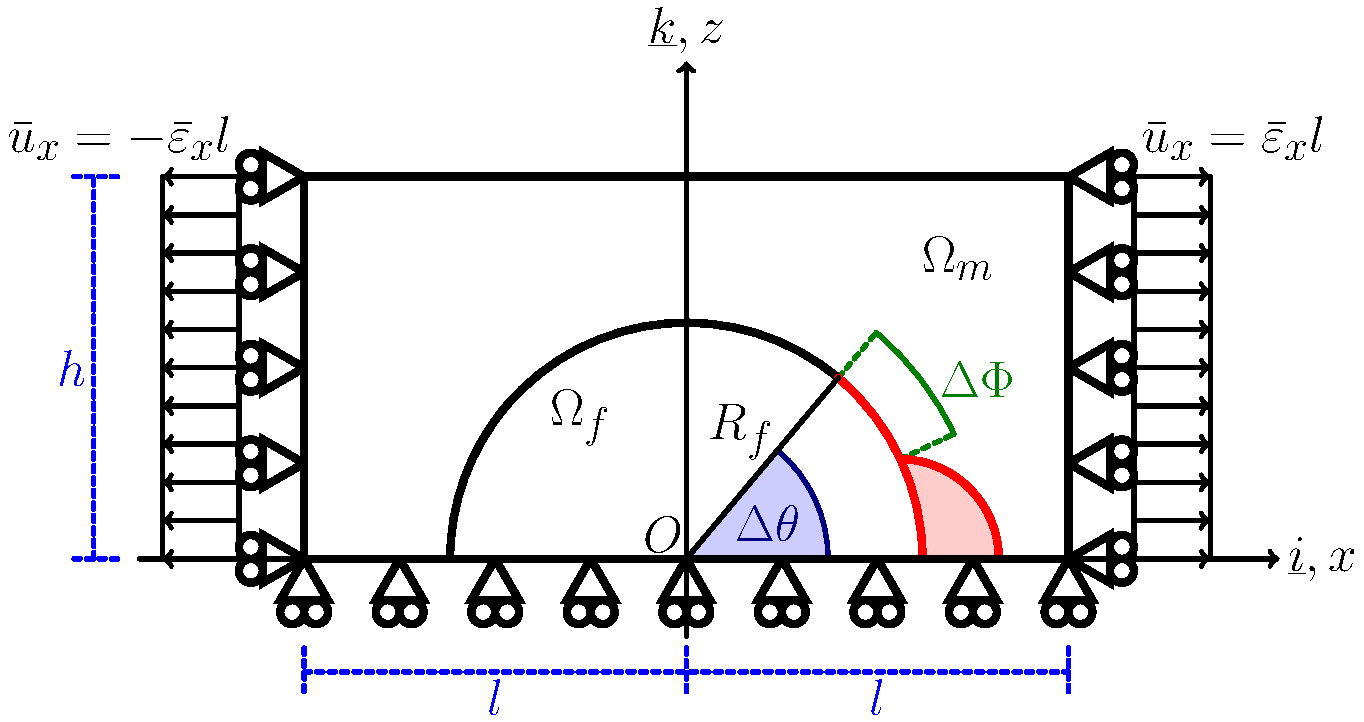
\includegraphics[width=\textwidth]{RUC.pdf}
        \caption{Schematic of the model with its main parameters.}\label{subfig:modelschem}
    \end{subfigure} ~
    \begin{subfigure}[b]{0.4\textwidth}
        \includegraphics[width=\textwidth]{mesh-detail.eps}
        \caption{Mesh near the crack tip. Crack's faces shown in red.}\label{subfig:meshdetail}
    \end{subfigure}

\caption{Details and main parameters of the Finite Element model.}\label{fig:FEmodel}
\end{figure}

The debond is placed symmetrically with respect to the $x$ axis (in red in~\ref{subfig:modelschem}) and has an angular size of $\Delta\theta$ (the full debond's size is thus $2\Delta\theta$). For large debond's sizes ($\geq 60^{\circ}-80^{\circ}$), a region of variable size $\Delta\Phi$ appears at the crack tip in which the crack faces are in contact and slide on each other. Due to its appearance, frictionless contact is considered between the two crack's faces to allow free sliding and avoid interpenetration. Symmetry with respect to the $x$ axis is applied on the lower boundary and kinematic coupling on the $x$-displacement along the left and right sides. The upper boundary is in general free, except for the model $1\times 1-coupling$ (Fig.~\ref{fig:thickplyalldebonds}) which requires kinematic coupling of vertical displacements also on the upper side. Constant $x$-displacement $\pm\varepsilon l$, corresponding to transverse strain $\varepsilon$ equal to $1\%$ is applied to the right and left boundaries.

\begin{table}[!htbp]
 \centering
 \caption{Summary of the mechanical properties of fiber and matrix.}
 \begin{tabular}{cccc}
\textbf{Material} & \textbf{$E\left[GPa\right]$}\ & \textbf{$G\left[GPa\right]$} & \textbf{$\nu\left[-\right]$} \\
\midrule
Glass fiber    & 70.0  & 29.2   & 0.2  \\
Epoxy    & 3.5    & 1.25   & 0.4
\end{tabular}
\label{tab:phaseprop}
\end{table}

The model is meshed using second order, 2D, plane strain triangular (CPE6) and rectangular (CPE8) elements. A regular mesh of quadrilateral elements with an almost unitary aspect ratio is required at the crack tip, as shown in Fig.~\ref{subfig:meshdetail}. The angular size $\delta$ of an element in the crack tip region is always equal to $0.05^{\circ}$. The crack faces are modeled as element-based surfaces and a small-sliding contact pair interaction with no friction is established between them. The Mode I, Mode II and total Energy Release Rates (ERRs) (respectively referred to as $G_{I}$, $G_{II}$ and $G_{TOT}$) represent the main output of the FEM analysis; they are evaluated using the VCCT technique~\cite{Krueger2004} implemented in a custom Python routine and, for the total ERR, the J-integral~\cite{Rice1968} by application of the Abaqus built-in functionality. A glass fiber-epoxy system is considered in every model, and it is assumed that their response lies always in the linear elastic domain. The properties used are listed in Table~\ref{tab:phaseprop}.

\subsection{Validation of the model}

The model is validated in Fig.~\ref{fig:validation} against the results reported in~\cite{Paris2007,Sandino2016}, obtained with the Boundary Element Method (BEM) for a single fiber with a symmetric debond placed in an infinite matrix. This situation is modeled using the \textit{free} RVE with $V_{f}=0.0079\%$, which corresponds to a RUC's length and height of $\sim 100$.

\begin{figure}[!h]
\centering
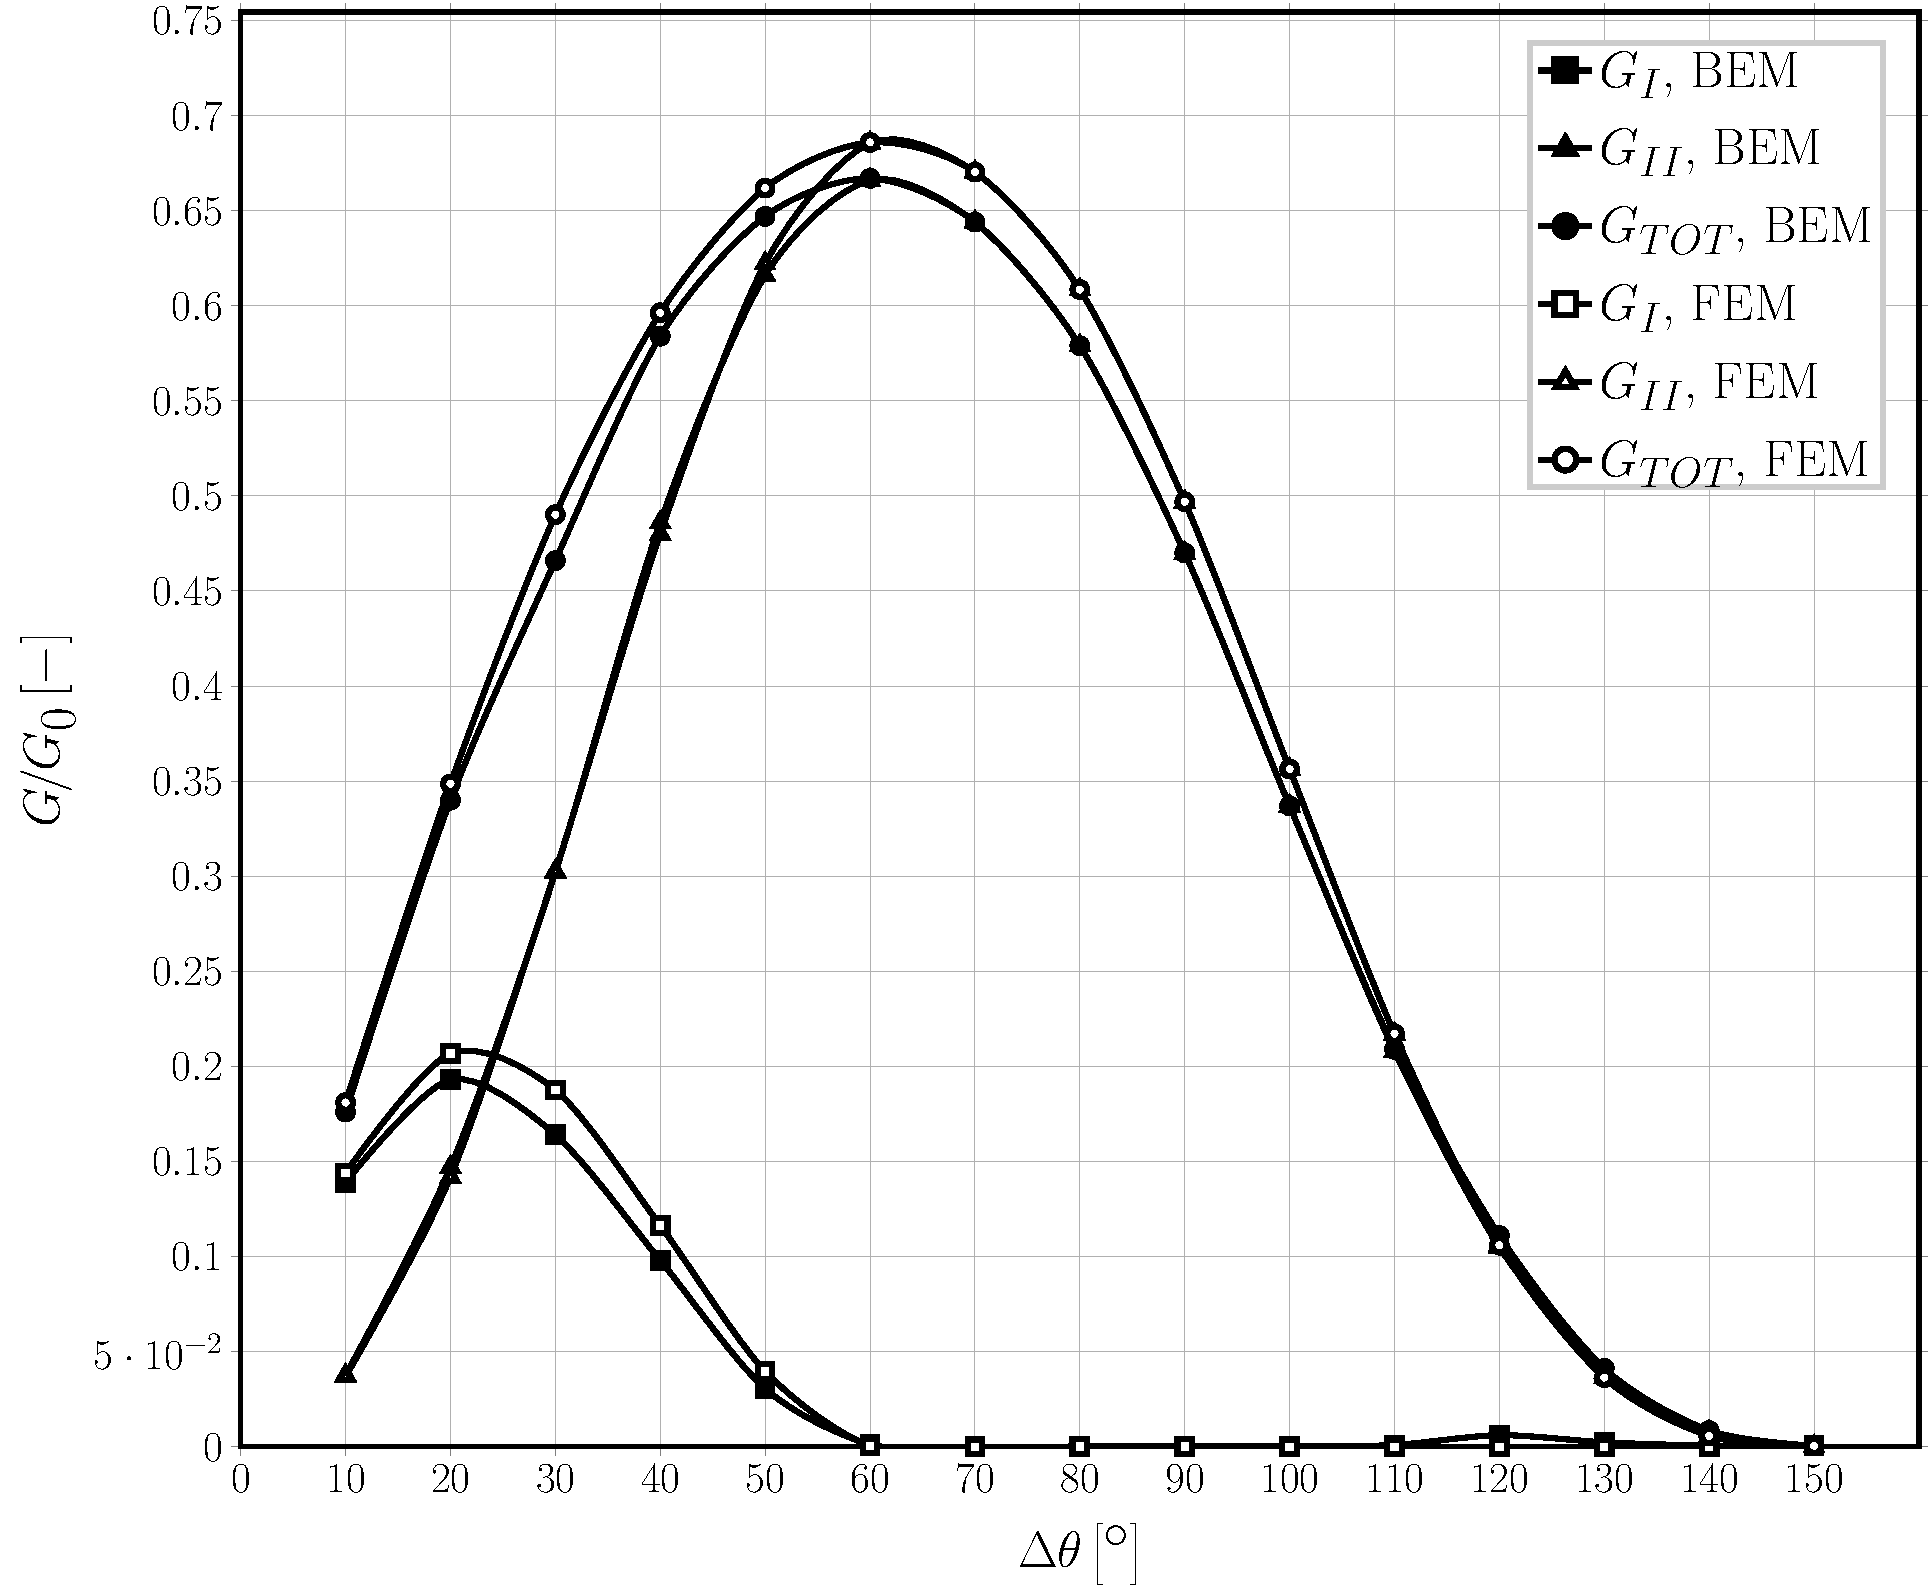
\includegraphics[width=\textwidth]{validation-VCCT.pdf}
\caption{Validation of the single fiber model for the infinite matrix case with respect to the BEM solution in \cite{Sandino2016}.}\label{fig:validation}
\end{figure}

To allow for a comparison, the results are normalized following~\cite{Sandino2016} with respect to a reference Energy Release Rate $G_{0}$ defined as

\begin{equation}
G_{0}=\frac{1+k_{m}}{8\mu_{m}}\sigma_{0}^{2}\pi R_{f}
\end{equation}

where $\mu$ is the shear modulus, $k$ is the Kolosov's constant defined as $3-4\nu$ for plane strain conditions, $R_{f}$ is the fiber radius and the index $m$ refers to the properties of the matrix. $\sigma_{0}$ is the stress at the boundary, computed as the average of the stress extracted at each boundary node along the right side (arithmetic average as nodes are equispaced by design along both the left and right sides). The agreement is good: the difference between the BEM solution, which is considered more accurate, and the FEM solution does not exceed $5\%$. The ERRs' maxima are in the same positions and the size of the contact zone is the same.  Nevertheless, an analysis of phenomena leading to less than $5\%$ differences in ERR would not be reliable and, therefore, it is not recommended.

%%%%%%%%%%%%%%%%%%%%%%%%%%%%%%%%%%%%%%%%%%%%%%%%%%%%%%%%%%%%%%%%%%%
%%%%%%%%%%%%%%%%%%%%%%%%%%%%%%%%%%%%%%%%%%%%%%%%%%%%%%%%%%%%%%%%%%%

\section{Results \& Discussion}

\subsection{Effect of Fiber Volume Fraction}\label{subsec:volfrac}

As shown in Figs.~\ref{fig:volumefractionMI} and~\ref{fig:volumefractionMII}, respectively for Mode I and Mode II, the fiber content has a drastic effect on the Energy Release Rate at the tip of the fiber/matrix interface crack. The effect of four levels of fiber volume fraction are compared, $30\%$, $50\%$, $60\%$ and $65\%$, on two microstructural models: a $11\times 11-free$ (every $11^{th}$ fiber in the central fiber row is partially debonded and, on the top of this row, we have 5 undamaged fiber rows), Figs.~\ref{subfig:volfracsmallerMI} and~\ref{subfig:volfracsmallerMII}, and a $21\times 21-free$ (every $21^{th}$ fiber in the central fiber row is partially debonded and, on the top of this row, we have 10 undamaged fiber rows), Figs.~\ref{subfig:volfracbiggerMI} and~\ref{subfig:volfracbiggerMII}.

\begin{figure}[!h]
\centering
    \begin{subfigure}[b]{0.475\textwidth}
        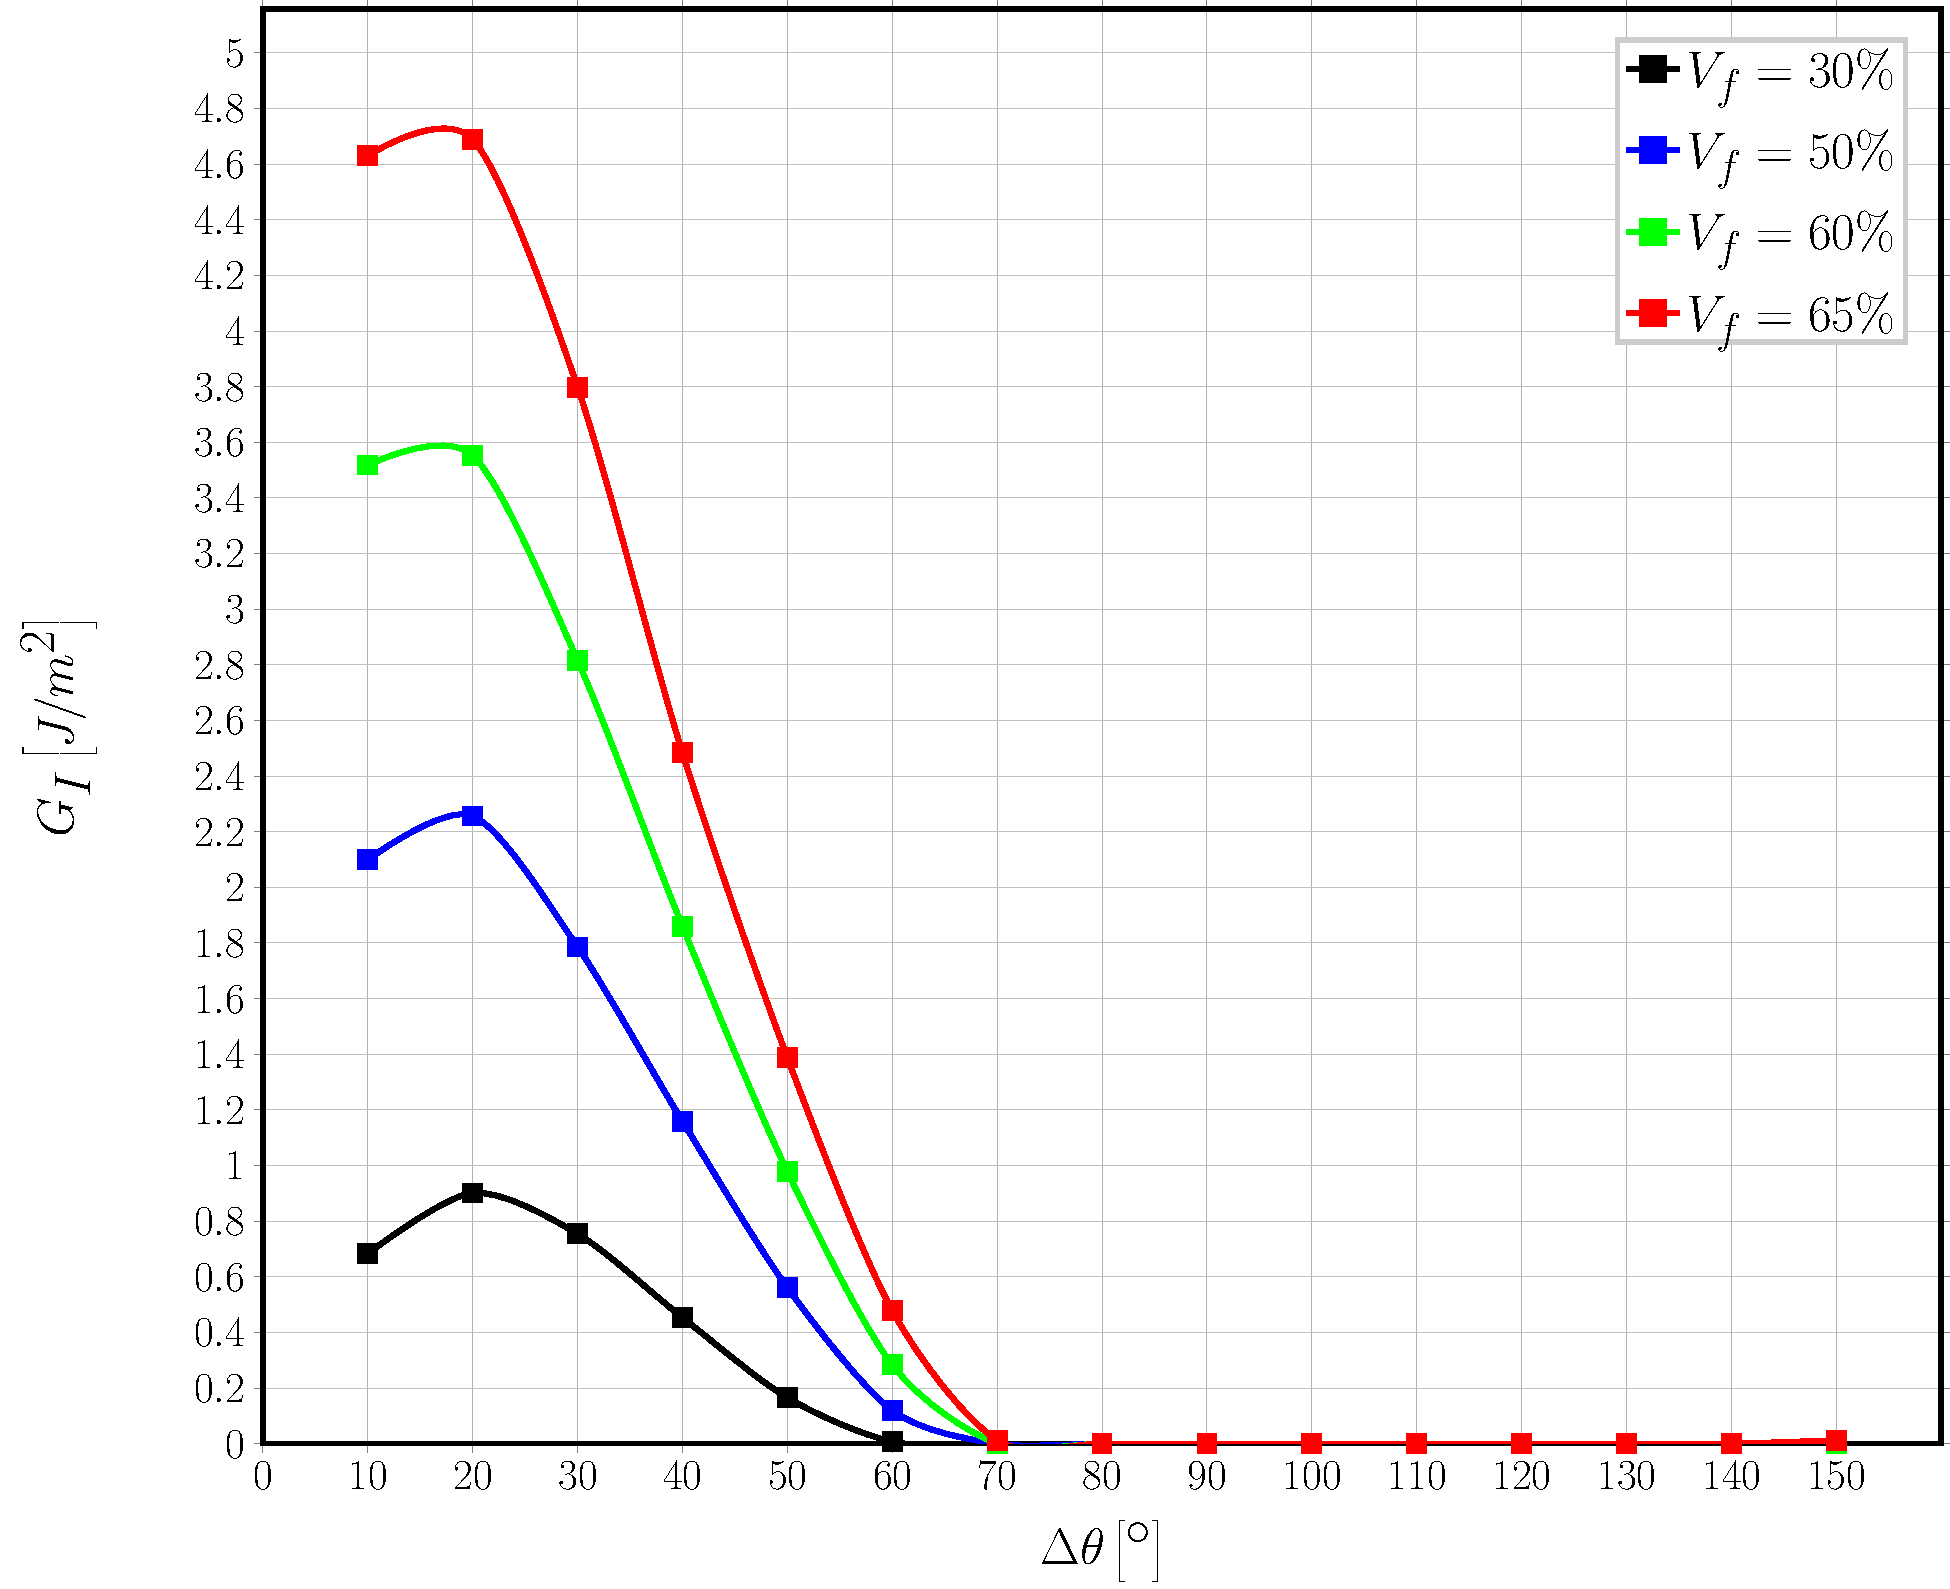
\includegraphics[width=\textwidth]{vf-smallermodel-GI.pdf}
        \caption{Model $11\times 11-free$.}\label{subfig:volfracsmallerMI}
    \end{subfigure} ~
    \begin{subfigure}[b]{0.475\textwidth}
        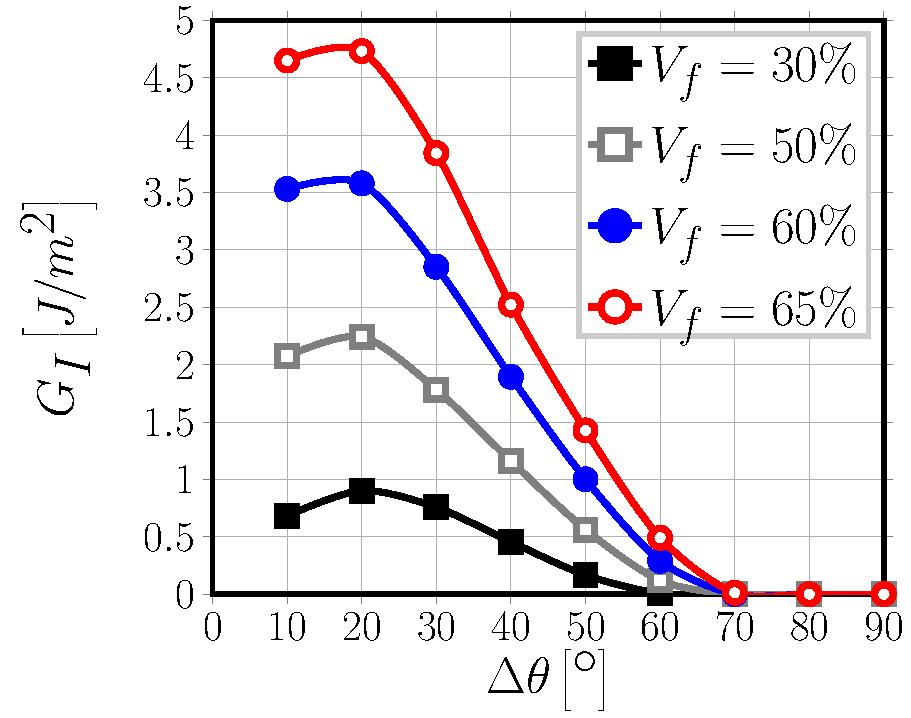
\includegraphics[width=\textwidth]{vf-biggermodel-GI.pdf}
        \caption{Model $21\times 21-free$.}\label{subfig:volfracbiggerMI}
    \end{subfigure}

\caption{A view of the effect of fiber volume fraction on Mode I ERR in two exemplificative models, subject to an applied transverse strain $\varepsilon_{x}$ of $1\%$.}\label{fig:volumefractionMI}
\end{figure}

Comparing Fig.~\ref{subfig:volfracsmallerMI} with~\ref{subfig:volfracbiggerMI}, and Fig.~\ref{subfig:volfracsmallerMII} with~\ref{subfig:volfracbiggerMII}, we can observe that the ERRs' values are very similar for RUCs with 11 × 11 and 21 × 21 fibers, though they are slightly higher for the larger RUC where the next debonded fiber and the free surface are further away from the debonded fiber. From these results we conclude that both RUCs are large enough to represent a single debonded fiber in an infinite array of bonded fibers. Obviously, there exists a specific effect of the fiber content. For Mode I, Fig.~\ref{fig:volumefractionMI}, the maximum value of the ERR increases by $\sim 5.2$ times when $V_{f}$ changes from $30\%$ to $65\%$. The debond's angular size for which the peak value occurs remains unchanged at $20^{\circ}$, but for $V_{f}=60\%$ and $65\%$ the Mode I ERR at $10^{\circ}$ and at $20^{\circ}$ are rather similar, approximately creating a plateau. Furthermore, increasing the fiber volume fraction delays the onset of the contact zone, which corresponds in Fig.~\ref{fig:volumefractionMI} to the first value of $\Delta\theta$ for which $G_{I}$ is equal to zero. For $V_{f}=30\%$, the contact zone first appears for a debond of $60^{\circ}$, similarly to what happens in the single fiber in infinite matrix model (Fig.~\ref{fig:validation}). For higher fiber contents, the contact zone's onset is delayed to a debond's size approximately equal to $70^{\circ}$.

\begin{figure}[!h]
\centering
    \begin{subfigure}[b]{0.475\textwidth}
        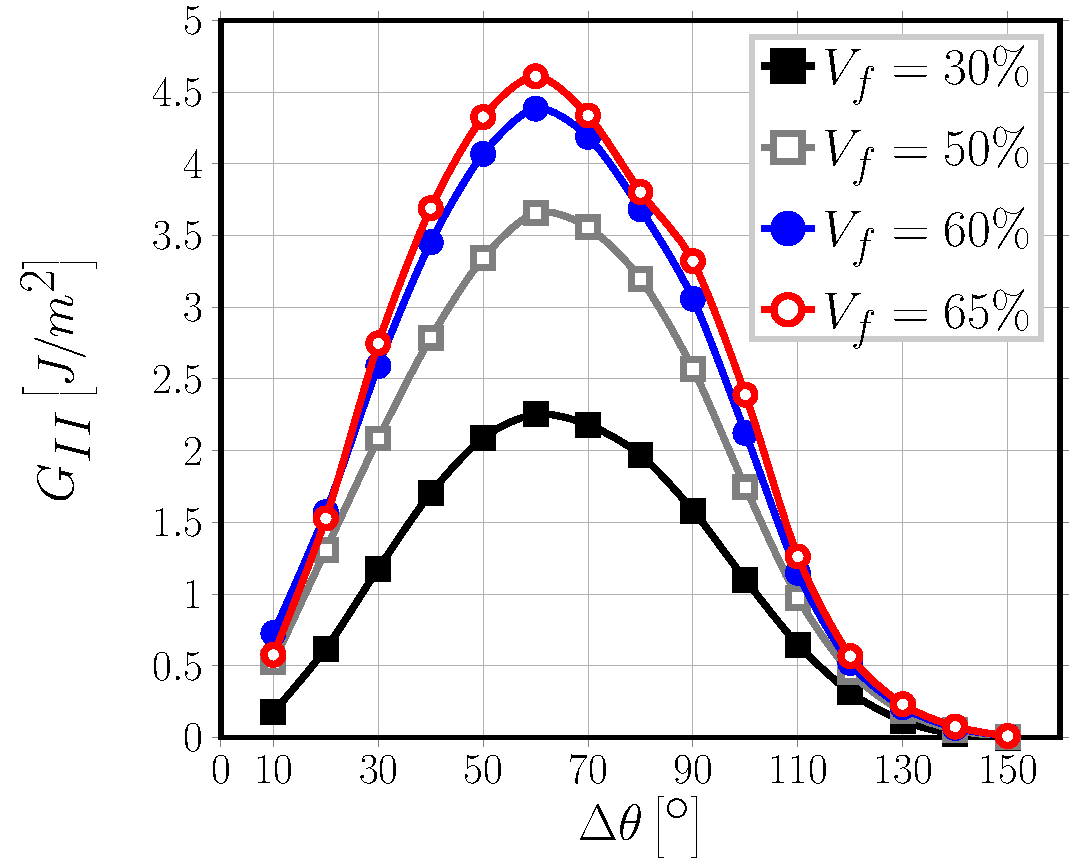
\includegraphics[width=\textwidth]{vf-smallermodel-GII.pdf}
        \caption{Model $11\times 11-free$.}\label{subfig:volfracsmallerMII}
    \end{subfigure} ~
    \begin{subfigure}[b]{0.475\textwidth}
        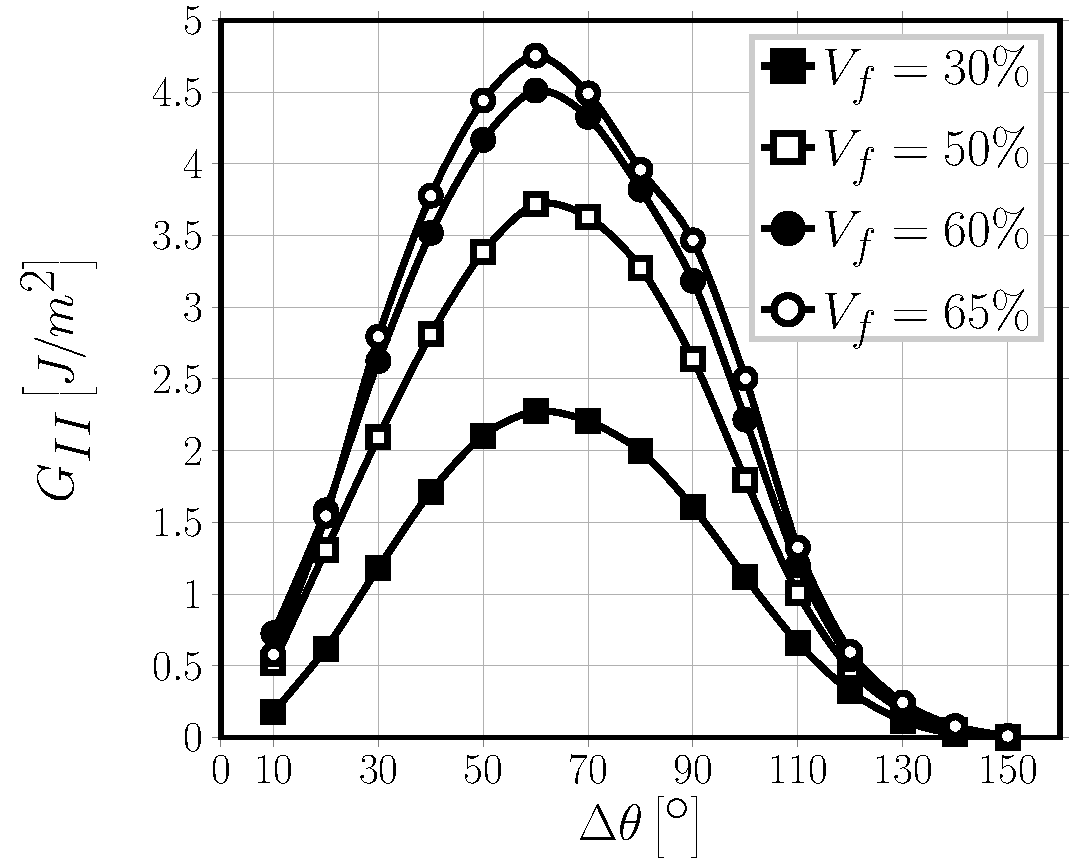
\includegraphics[width=\textwidth]{vf-biggermodel-GII.pdf}
        \caption{Model $21\times 21-free$.}\label{subfig:volfracbiggerMII}
    \end{subfigure}

\caption{A view of the effect of fiber volume fraction on Mode II ERR in two exemplificative models, subject to an applied transverse strain $\varepsilon_{x}$ of $1\%$.}\label{fig:volumefractionMII}
\end{figure}

For Mode II, Fig.~\ref{fig:volumefractionMII}, the maximum value of the ERR increases by $\sim 2.1$ times when $V_{f}$ changes from $30\%$ to $65\%$. The effect is thus similar to Mode I, but with a significantly lower magnitude. Similar to Mode I, the debond's size for which the peak value of Mode II occurs remains unchanged, at $60^{\circ}$. There is a distinct maximum in the curve and its shape does not dependon the fiber content. It is worthwhile to notice that the ratio of Mode II to Mode I peak values is $\frac{max\left(G_{II}\right)}{max\left(G_{I}\right)}\sim\frac{2.2}{0.9}\sim 2.4$ for $V_{f}=30\%$, while it is $\sim\frac{4.7}{4.7}\sim 1$ for $V_{f}=65\%$. Given that the peaks occur at different debond's sizes, for which the value of the other ERR is very small or even close to zero, this means that the increase in fiber content creates a long range of very close values of the total ERR, that may have a global destabilizing effect on the debond's growth.\\
The general increasing trends observed in Figs.~\ref{fig:volumefractionMI} and~\ref{fig:volumefractionMII} are related to the fact that, given that the global and local $V_{f}$ are everywhere identical in the models presented, an increase in fiber content corresponds to a decrease in the average distance between fibers. Thus, the decay of the local stress and strain fields in the matrix domain occurs over smaller lengths causing higher values at the crack tip. The difference in relative magnitude between Mode I and Mode II and the delay in the contact zone's onset are instead due to the interplay between two different mechanisms, both caused by the ordered microstructural arrangement of the model. In the models considered, a fully bonded fiber is always placed along the horizontal direction, aligned with the partially debonded fiber and exactly in front of the debond. By increasing $V_{f}$, the former moves closer to the latter and for small debonds this causes a magnification of the x-strain at the crack tip. For small debonds ($\leq 20^{\circ}-30^{\circ}$) in fact, the crack tip is approximately normal to the $x$-direction and thus an increase in $\varepsilon_{x}$ causes an increase in $G_{I}$. On the other hand, for large debonds ($\geq 70^{\circ}-80^{\circ}$) the crack growth direction is almost aligned with the $x$-axis, thus a magnification in the $x$-strain translates into an increase of Mode II ERR. However, this increasing effect on $G_{II}$ is partially counteracted by the presence of a fully bonded fiber on top of the debonded fiber and aligned with it. As fibers are more rigid than the surrounding matrix, the presence of the former will restrain horizontal displacements, thus hampering strong increases in $G_{II}$ for large debonds. Furthermore, due to the mismatch in the Poisson's ratios, the fully bonded fiber placed above generates an upward-directed component of the vertical displacement field in the matrix, which tends to open the debond and causes the delay in the contact zone's onset. The interplay between these mechanisms is governed by the average inter-fiber distance and, in turn, by the fiber volume fraction.\\
These observations are in strong agreement with the results reported in~\cite{Sandino2016}, where the effect on the ERR of a partially debonded fiber of two fully bonded nearby fibers, placed symmetrically with respect to the loading direction, is studied for different angular positions (denoted as $\theta_{2}$) and radial distances in a model with an effectively infinite matrix ($V_{f}\sim0.09\%$). The effect of the former is studied for a constant value of the radial distance between the debonded and bonded fibers, which corresponds to a local $V_{f}^{local}$ of $\sim62\%$ assuming hexagonal packing. They report an increase in both Mode I and Mode II ERR with respect to the single fiber case when the two fibers are placed at an angle of respectively $\pm25^{\circ},\pm30^{\circ},\pm140^{\circ},\pm150^{\circ},\pm155^{\circ}$, i.e. closest to the loading direction. Notice that for $\pm25^{\circ}$ and $\pm155^{\circ}$ the two fully bonded fibers are almost in contact, with an inter-fiber distance of $\sim0.04$ times their radius. This result confirms the considerations made in the previous paragraph about the $x$-strain magnification caused by the presence of fully bonded fibers along the loading direction. The effect is further analyzed and discussed in Sec.~\ref{subsec:singlefiberud} and Sec.~\ref{subsec:multrow}. In the range $\pm40^{\circ}-\pm130^{\circ}$ instead, the presence of the other fibers causes a reduction of the ERR and, particularly in the range $80^{\circ}-120^{\circ}$, results are very close and almost insensitive to variations in $\theta_{2}$, which supports the previous conclusion about the effect of a fully bonded fiber on top the partially debonded one. This effect is treated in more detail in Sec.~\ref{subsec:fiberabove}.\\
Comparing the results from~\cite{Sandino2016} with those presented in this paper, an hypothesis can be furthermore formulated about the robustness of the results of the present article with respect to deviations in fiber position: it seems reasonable to assume a tolerance to deviations of max. $\pm30^{\circ}$ with respect to the loading direction and of max. $\pm20^{\circ}$ with respect to the through-the-thickness direction.\\
The effect of the local fiber content is also investigated in~\cite{Sandino2016}, by changing the radial distance between the partially debonded fiber and the fully bonded ones. They observe that the further the fully bonded fibers are placed from the central one, i.e. the lower the local $V_{f}$, the lower is their effect on the ERR. The magnitude of the effect is however small: the maximum increase of the total ERR is of $\sim1.15$ times for $\theta_{2}=30^{\circ}$ and $150^{\circ}$ when increasing $V_{f}^{local}$ from $28\%$ to $62\%$; of $\sim1.25$ times for $\theta_{2}=60^{\circ}$, $\sim1.4$ times for $\theta_{2}=90^{\circ}$ and $\sim1.75$ times for $\theta_{2}=120^{\circ}$ when decreasing $V_{f}^{local}$ from $62\%$ to $28\%$. Analogous results can be found in~\cite{Zhuang2018}, where the authors consider a centrally-placed partially debonded fiber sorrounded by an hexagonal cluster inside an homogenized UD composite. They observe a reduction in the ERR when the local fiber volume fraction is increased, i.e. when the spacing between fibers is reduced. The strongest change is reported for Mode II, which registers a maximum increase of $\sim1.36$ times when the local fiber volume fraction is decreased from $78\%$ to $66\%$. Thus, the trends presented in~\cite{Sandino2016,Zhuang2018} agree with the results on the effect of $V_{f}$ and support the considerations made so far. The stark difference in magnitude however highlights the contrast between the effect of the local $V_{f}$ of a cluster of fibers inside an infinite medium and of the global $V_{f}$ of long-range microstructural arrangements, such the ones considered in this article. In the former, the fiber volume fraction controls the size of a localized perturbation to a constant elastic solution; in the latter, $V_{f}$ determines the characteristic lengths of a global periodic solution.

\subsection{Interaction between debonds in UD composites with a single row of fibers}\label{subsec:singlefiberud}

The interaction of debonds appearing at regular intervals in an ultra-thin UD composite with a single row of fibers is studied for Mode I (Fig.~\ref{fig:sidefibersMI}) and Mode II (Fig.~\ref{fig:sidefibersMII}) and fiber content equal to $30\%$ (Figs.~\ref{subfig:sidefiber30MI} and~\ref{subfig:sidefiber30MII}) and $60\%$ (Figs.~\ref{subfig:sidefiber60MI} and~\ref{subfig:sidefiber60MII}). The models treated are $3\times 1-free$, $5\times 1-free$, $7\times 1-free$, $11\times 1-free$, $21\times 1-free$, $101\times 1-free$ and $201\times 1-free$, corresponding respectively to a debond every $3^{rd}$, $5^{th}$, $7^{th}$, $11^{th}$, $21^{st}$, $101^{st}$ and $201^{st}$ fiber (Fig.~\ref{subfig:freethinply}). Given that the upper surface of the UD row is left free, the interaction with the debonded fiber in the next RUC is stronger than in any other case and the results of this section are thus the most conservative in terms of debond's growth: the ERRs should be the largest. The effect is enhanced in composites with high $V_{f}$ and especially for $G_{II}$: at $V_{f}=60\%$ the highest $G_{II}$ value for the $201\times 1-free$ composite in Fig.~\ref{subfig:sidefiber60MII} is more than $3$ times higher than the $G_{II}$ value value for the $21\times21-free$ composite in Fig.~\ref{subfig:volfracbiggerMII}. Even the maximum is shifted to larger angles. The $G_{I}$ value is only 30\% higher.\\
From both Fig.~\ref{fig:sidefibersMI} and Fig.~\ref{fig:sidefibersMII}, it can be seen that the presence of a debond close to the analyzed debond decreases the strain magnification effect discussed in Sec.~\ref{subsec:volfrac} and thus reduces the value of the ERR. This phenomenon is called \say{crack shielding}~\cite{Garcia2015}.

\begin{figure}[!h]
\centering
    \begin{subfigure}[b]{0.475\textwidth}
        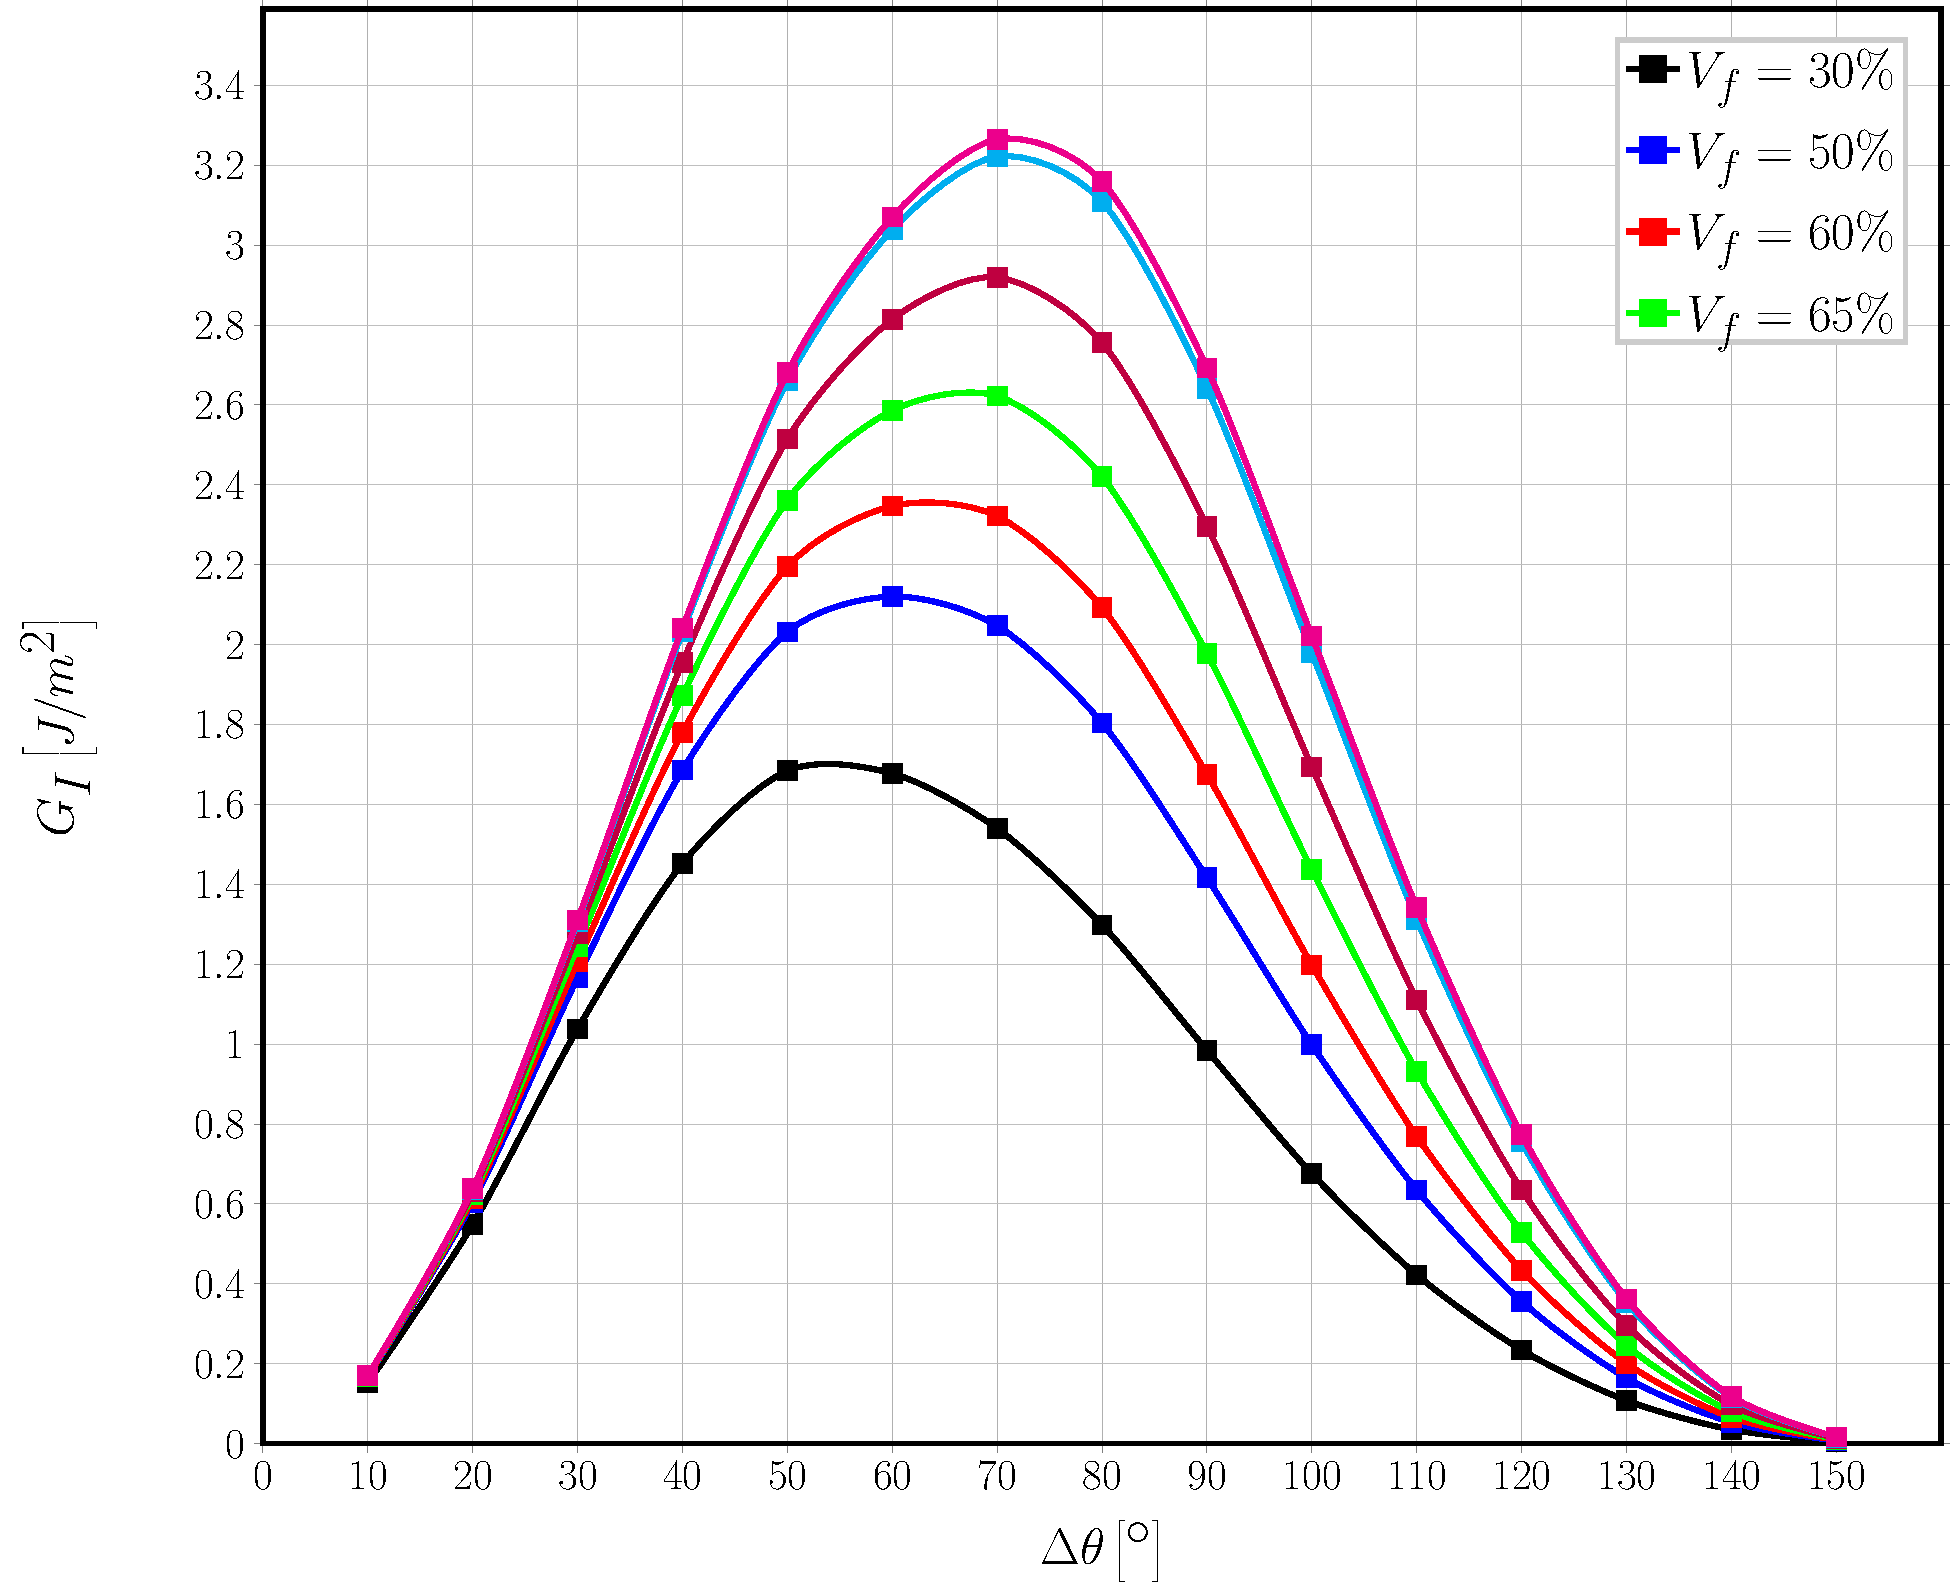
\includegraphics[width=\textwidth]{sidefibers-vf30-GI.pdf}
        \caption{$V_{f}=30\%$.}\label{subfig:sidefiber30MI}
    \end{subfigure} ~
    \begin{subfigure}[b]{0.475\textwidth}
        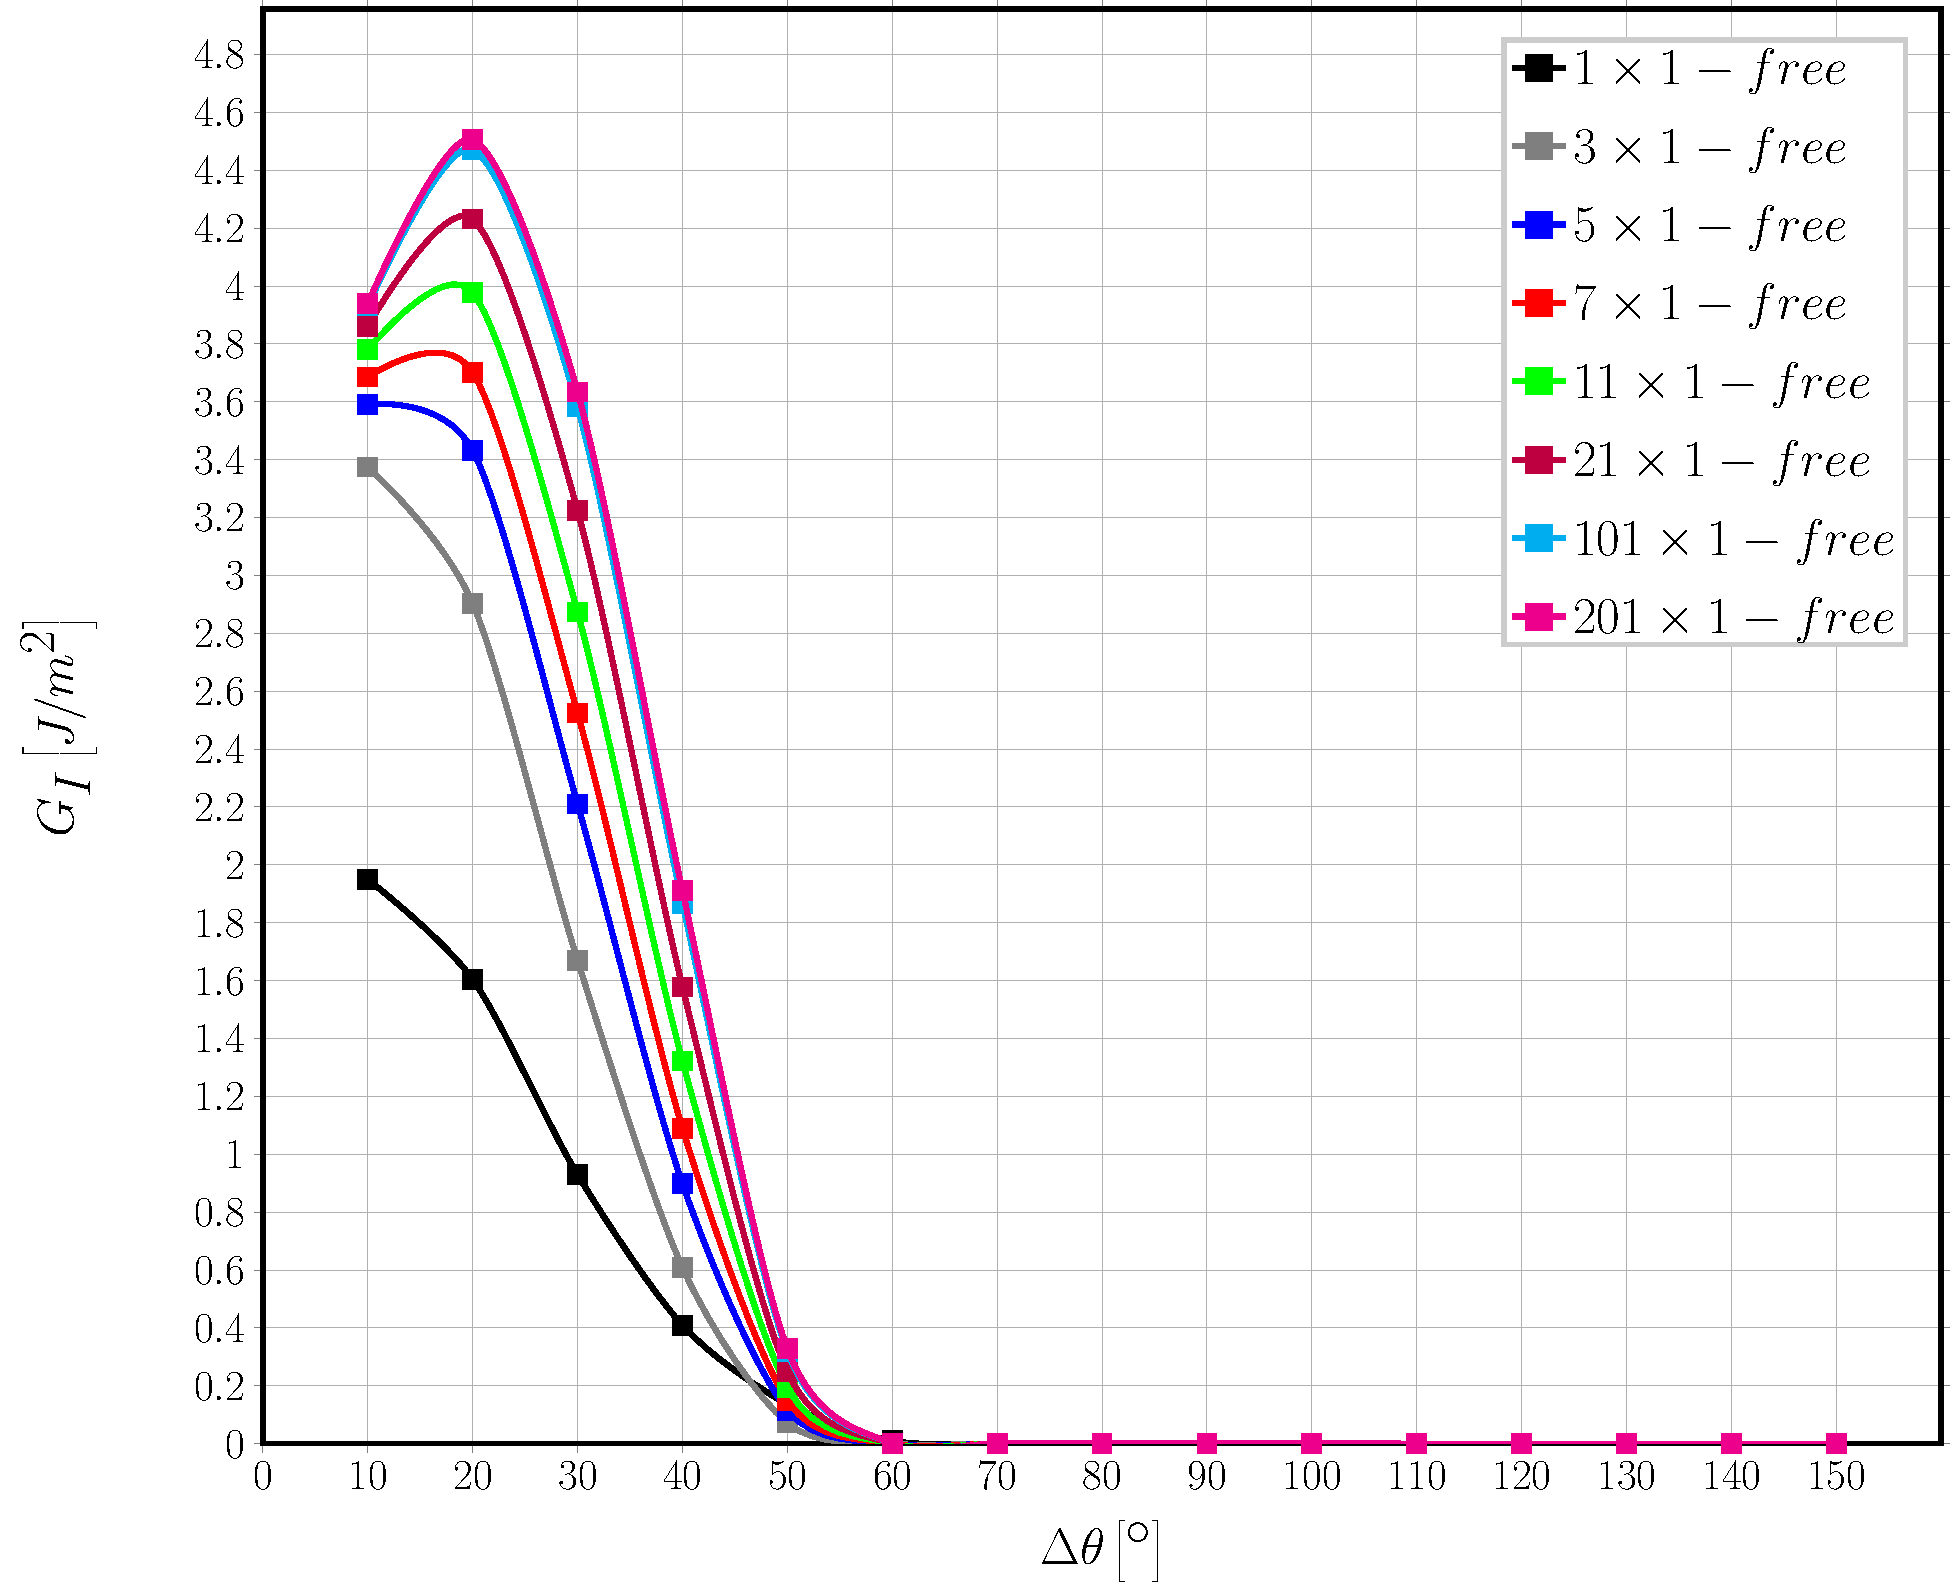
\includegraphics[width=\textwidth]{sidefibers-vf60-GI.pdf}
        \caption{$V_{f}=60\%$.}\label{subfig:sidefiber60MI}
    \end{subfigure}

\caption{Effect of the interaction between debonds appearing at regular intervals on Mode I ERR in an UD with a single layer of fibers at different levels of fiber volume fraction $V_{f}$, subject to an applied transverse strain $\varepsilon_{x}$ of $1\%$.}\label{fig:sidefibersMI}
\end{figure}

For Mode I, the presence of a free surface, and inversely the absence of a fully bonded fiber along the vertical direction, implies the absence of the counteracting upward-oriented vertical component of the displacement field due to the mismatch in Poisson's ratios. This in turn translates into the constancy of the value of $\Delta\theta$ corresponding to contact zone's onset, always equal to $60^{\circ}$. For $V_{f}=30\%$, Mode I is reduced when the spacing between debonds (in terms of number of fully bonded fibers between them in our models) decreases, but the magnitude of change is significant only when the spacing is reduced from a debond every $5^{th}$ fiber to one every $3^{rd}$. For comparison, the difference of peak $G_{I}$ values for $V_{f}=30\%$ between $5\times 1-free$ and $3\times 1-free$ is $\sim 0.2\ \frac{J}{m^{2}}$ (around $30\%$ of the lower value), while between $201\times 1-free$ and $5\times 1-free$ is $\sim 0.05\ \frac{J}{m^{2}}$ (around $7\%$ of the lower value). A similar observation can be made for $V_{f}=60\%$, but for larger spacings: no difference can be seen between the case of a debond placed every $101^{th}$ and every $201^{th}$ fiber. These observations suggest the existence of characteristic distance dependent on the fiber volume fraction which governs the interaction between debonds: in low $V_{f}$ composites ($V_{f}=30\%$) the convergence to a non-interactive solution is faster (less interaction between debonded fibers in neighboring RUCs).

\begin{figure}[!h]
\centering
    \begin{subfigure}[b]{0.475\textwidth}
        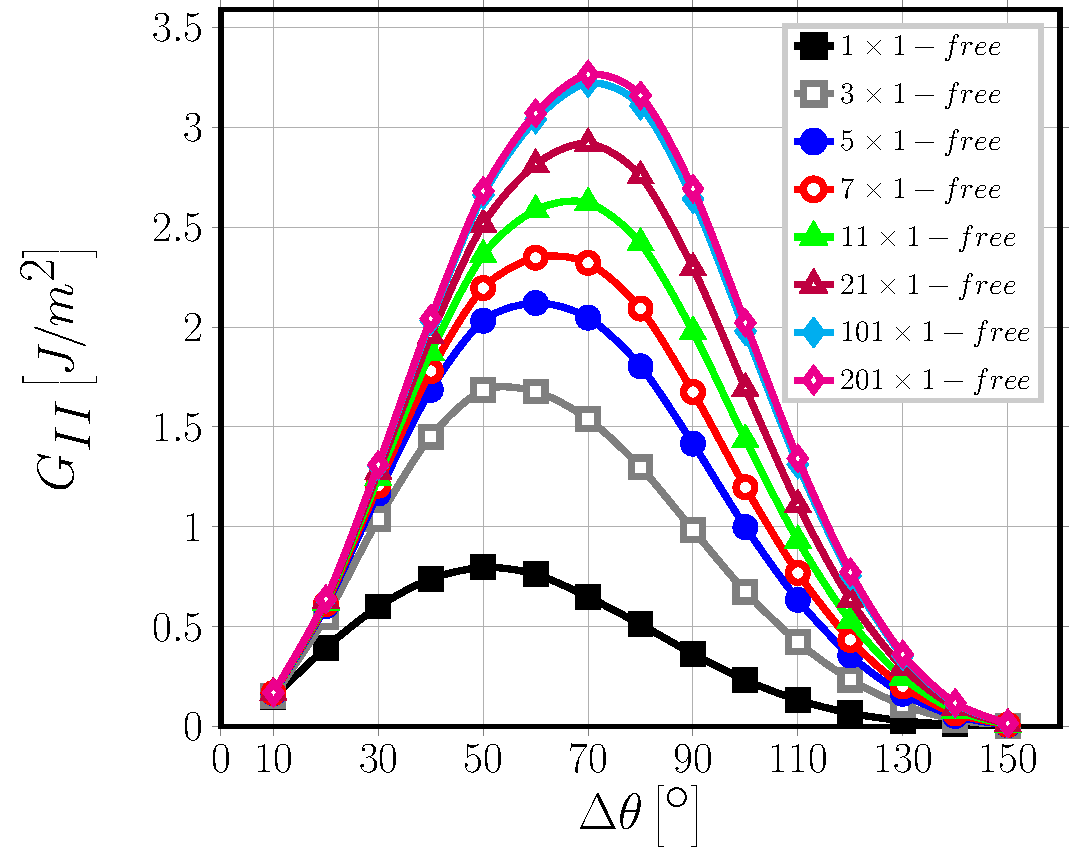
\includegraphics[width=\textwidth]{sidefibers-vf30-GII.pdf}
        \caption{$V_{f}=30\%$.}\label{subfig:sidefiber30MII}
    \end{subfigure} ~
    \begin{subfigure}[b]{0.475\textwidth}
        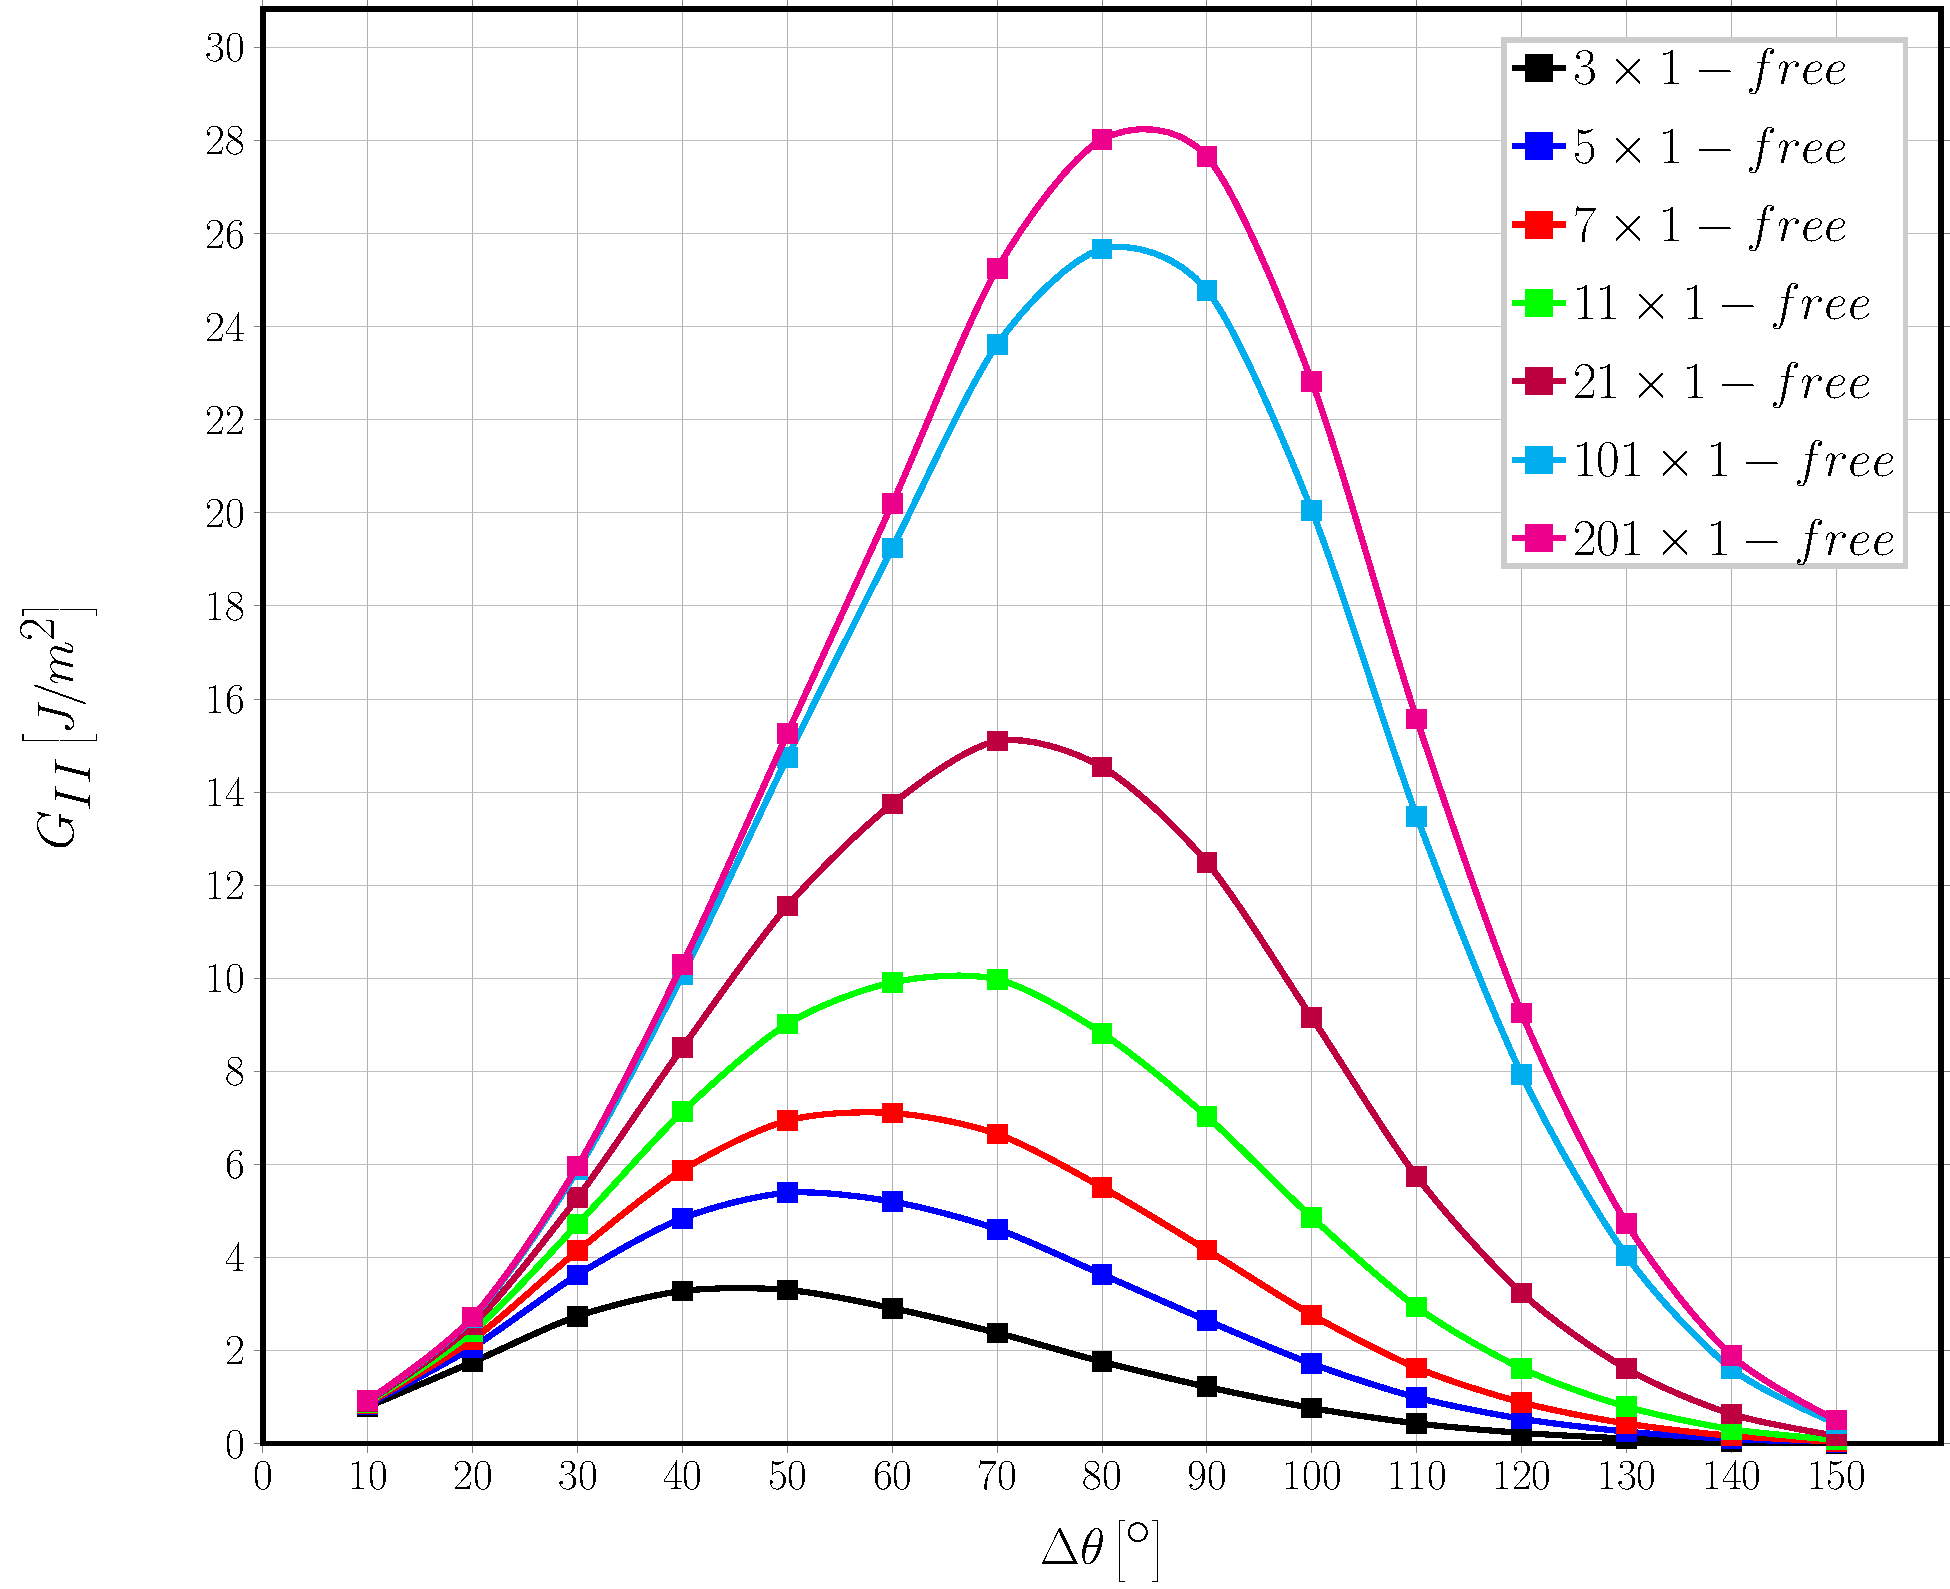
\includegraphics[width=\textwidth]{sidefibers-vf60-GII.pdf}
        \caption{$V_{f}=60\%$.}\label{subfig:sidefiber60MII}
    \end{subfigure}

\caption{Effect of the interaction between debonds appearing at regular intervals on Mode II ERR in a single-ply laminate with a single layer of fibers at different levels of fiber volume fraction $V_{f}$, subject to an applied transverse strain $\varepsilon_{x}$ of $1\%$.}\label{fig:sidefibersMII}
\end{figure}

Without costraint on the upper surface, the strain magnification effect creates a larger displacement gap in the $x$-direction, which increases Mode II for larger debonds. When debonds are far apart, the series of rigid elements in the ultra-thin composite row (constituted by fully bonded fibers and their surrounding matrix) creates higher $x$-strains than in average in the element with the debonded fiber, which in turn generates higher tangential displacements at the crack tip for larger debonds. Conversely, when debonds are closer (smaller number of rigid elements between them), the strain concentration in the debonded element is more similar to the applied strain (the magnification is reduced) and the tangential displacement component at the crack tip decreases for large $\Delta\theta$. This is the mechanism behind the change in the value of $\Delta\theta$ for which the peak of $G_{II}$ occurs: from $70^{\circ}$ to $50^{\circ}$ at $30\%$, and from $80^{\circ}$ to $40^{\circ}$ at $60\%$ going from the higher to the smaller spacing of debonds. Differently from Mode I, the presence of a characteristic distance is harder to establish. For $V_{f}=30\%$ (Fig.~\ref{subfig:sidefiber30MII}), it seems reasonable to establish it at around $100$ fully bonded fibers between each debond. For $V_{f}=60\%$ (Fig.~\ref{subfig:sidefiber60MII}), the difference between models $101\times 1-free$ and $201\times 1-free$ is still sizable, thus preventing the establishment of such characteristic distance. It is possible to observe, however, that the change between $101\times 1-free$ and $201\times 1-free$ is significantly smaller than between $21\times 1-free$ and $101\times 1-free$ ($2\left[\frac{J}{m^{2}}\right]$ vs $11\left[\frac{J}{m^{2}}\right]$), thus suggesting the existence of the characteristic distance outside the range studied. Nevertheless, one should question whether the single row composite with free surface is an appropriate RUC for defining the upper bound for $G_{II}$: $G_{II}$ may be more affected by the free surface than by the effect of the interaction between debonds in the row.

\subsection{Influence of rows of fully bonded fibers on debond's ERR in the middle row}\label{subsec:fiberabove}

The effect of the presence of rows of fully bonded fibers on debond's growth in the central row with all fibers partially debonded is studied for Mode I (Fig.~\ref{fig:abovefibersMI}) and Mode II (Fig.~\ref{fig:abovefibersMII}) and fiber content equal to $30\%$ (Figs.~\ref{subfig:abovefiber30MI} and~\ref{subfig:abovefiber30MII}) and $60\%$ (Figs.~\ref{subfig:abovefiber60MI} and~\ref{subfig:abovefiber60MII}). The models treated are $1\times 3-free$, $1\times 5-free$, $1\times 7-free$, $1\times 11-free$, $1\times 21-free$, $1\times 101-free$ and $1\times 201-free$, corresponding to a UD composite with respectively $3$, $5$, $7$, $11$, $21$, $101$ and $201$ rows of fibers (Fig.~\ref{subfig:thickplycentraldebonds}).

\begin{figure}[!h]
\centering
    \begin{subfigure}[b]{0.45\textwidth}
        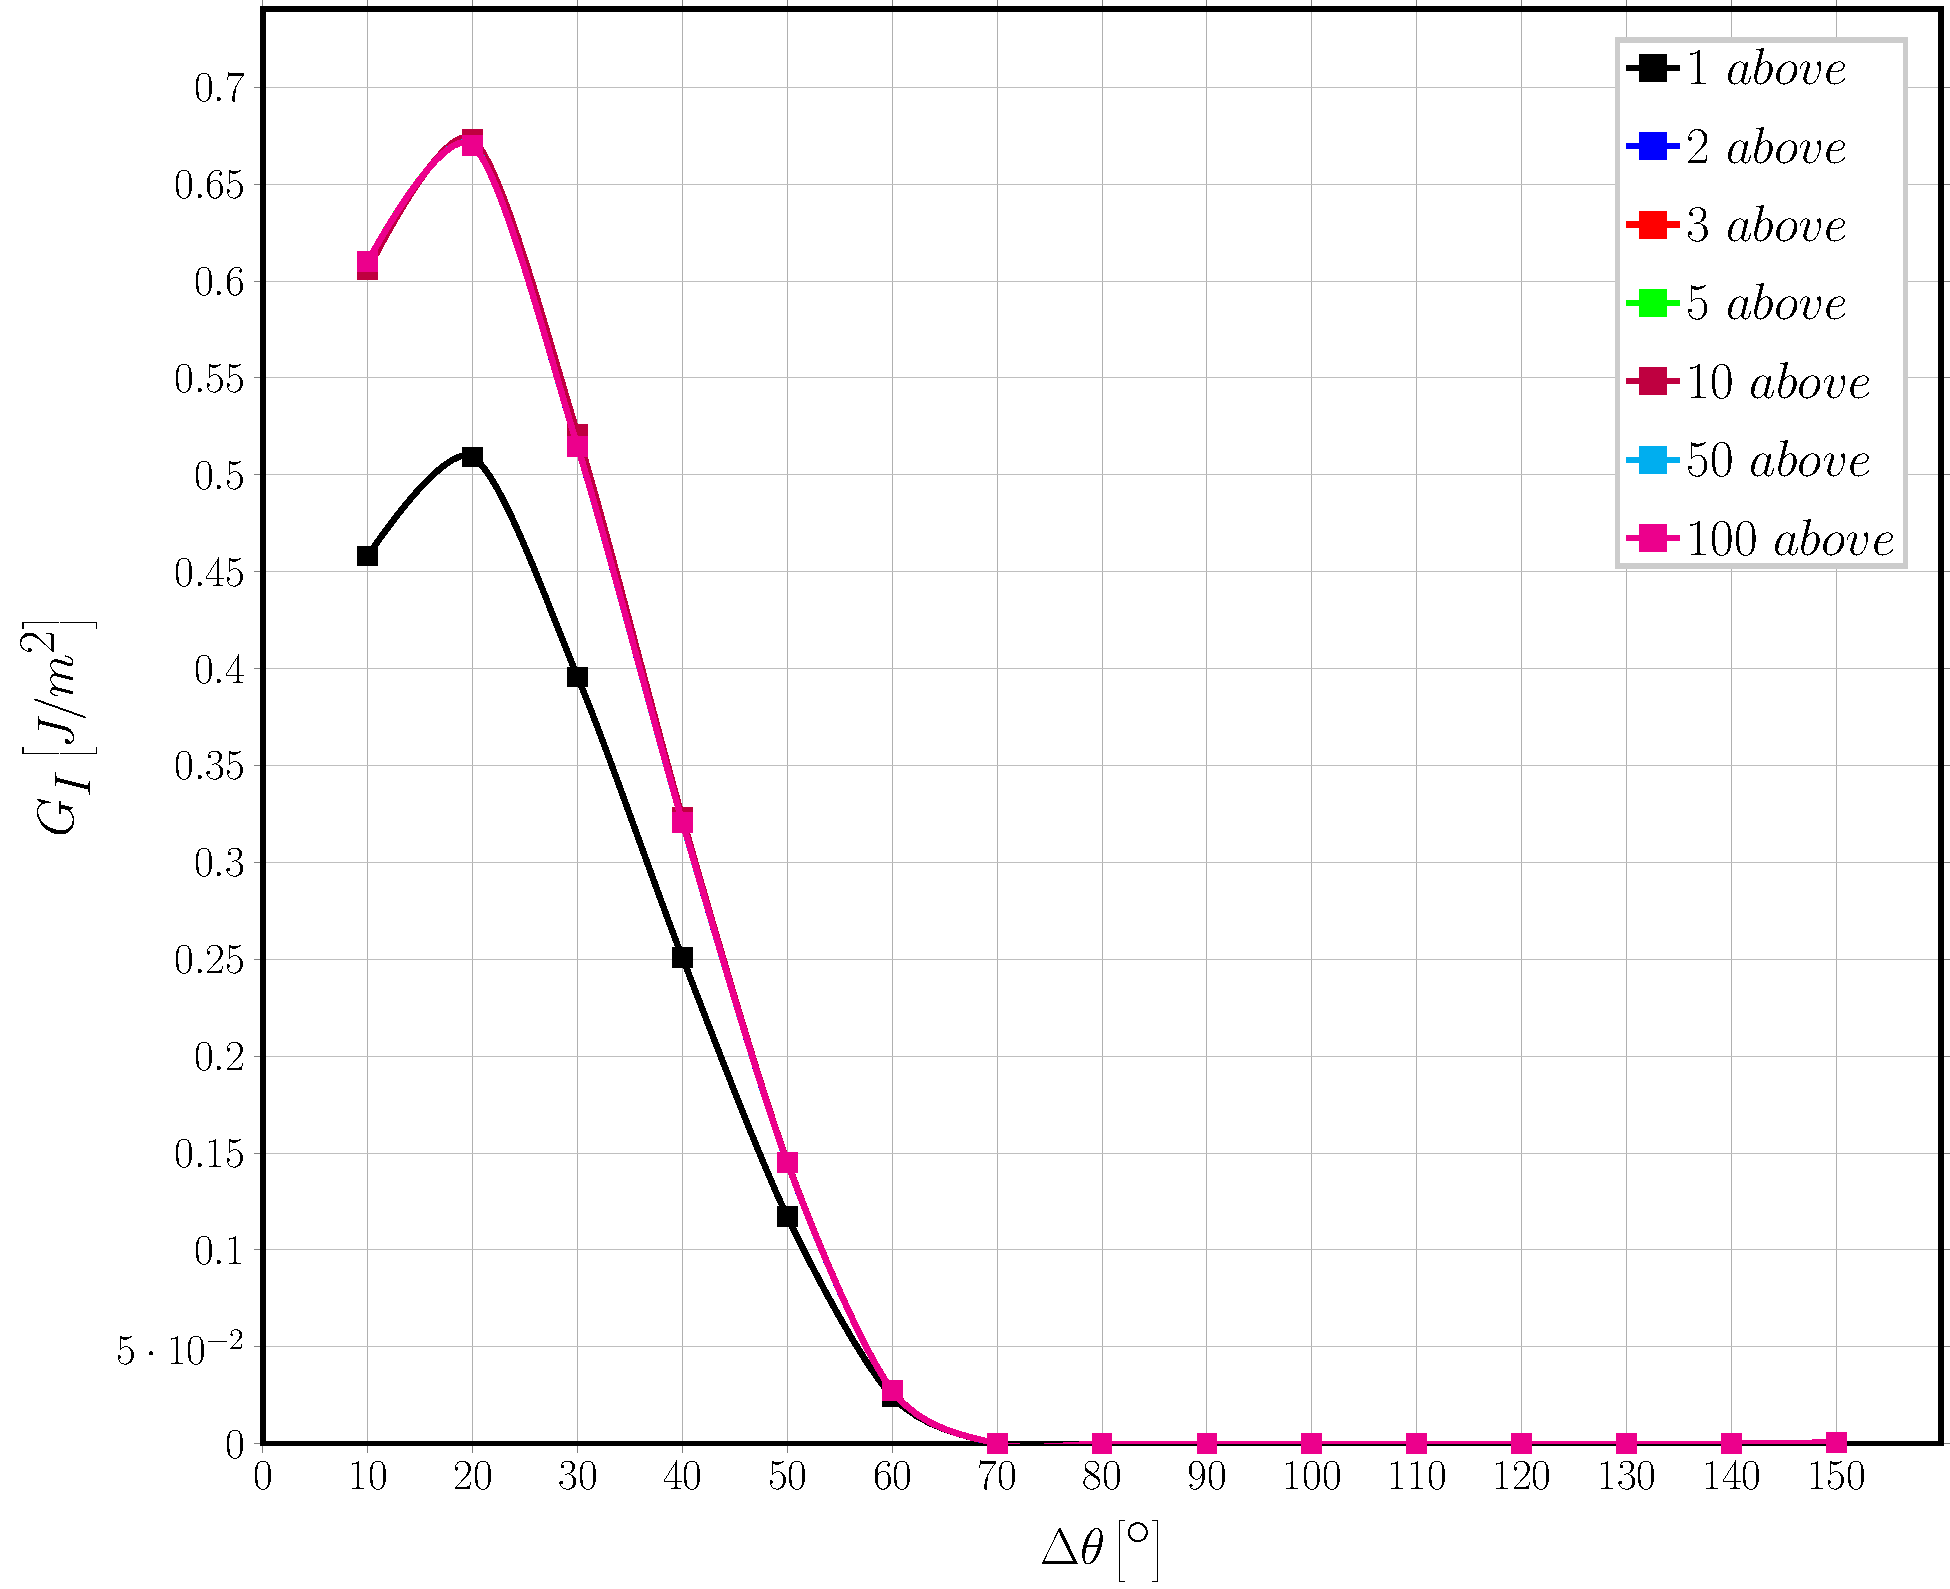
\includegraphics[width=\textwidth]{abovefibers-vf30-GI.pdf}
        \caption{$V_{f}=30\%$.}\label{subfig:abovefiber30MI}
    \end{subfigure} ~
    \begin{subfigure}[b]{0.45\textwidth}
        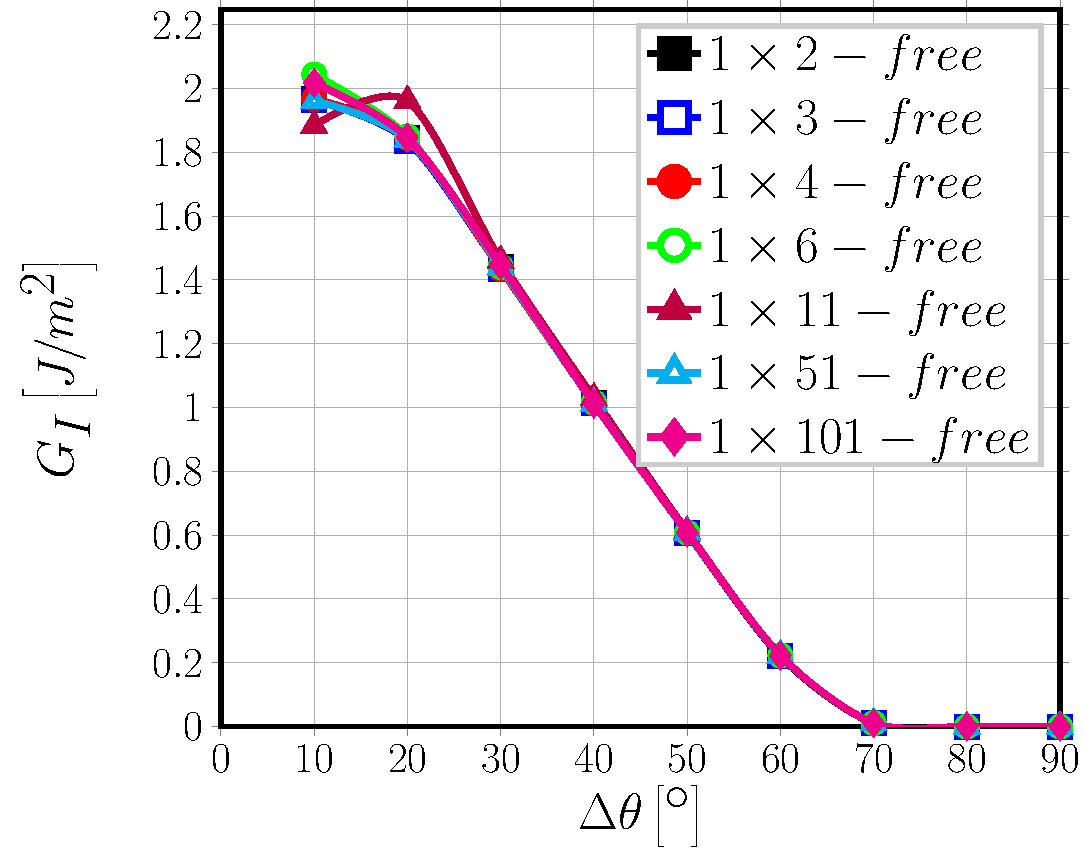
\includegraphics[width=\textwidth]{abovefibers-vf60-GI.pdf}
        \caption{$V_{f}=60\%$.}\label{subfig:abovefiber60MI}
    \end{subfigure}

\caption{Influence of layers of fully bonded fibers on debond's growth in Mode I ERR in a centrally located line of debonded fibers at different levels of fiber volume fraction $V_{f}$, subject to an applied transverse strain $\varepsilon_{x}$ of $1\%$.}\label{fig:abovefibersMI}
\end{figure}

The results shown strengthen the arguments made in Sec.~\ref{subsec:volfrac} and Sec.~\ref{subsec:singlefiberud}. It can, in fact, be seen in Fig.~\ref{fig:abovefibersMI} that an increasing number of bonded fiber rows across the thickness delays the onset of the contact zone to a debond of $70^{\circ}$ in size, due to the introduction of an additional positive component of the vertical displacement which translates into an opening displacement at the debond's tip.\\
Comparing Fig.~\ref{subfig:sidefiber60MII} with Fig.~\ref{subfig:abovefiber60MII}, we observe that the presence of bonded fiber rows significantly reduce the $G_{II}$ and its maximum is shifted back to $60^{\circ}$, thus confirming the hypothesis in Section~\ref{subsec:singlefiberud} that the absence of $G_{II}$ convergence with the increasing distance in a single-row composite is caused more by the free surface than by the interaction between debonds.

\begin{figure}[!h]
\centering
    \begin{subfigure}[b]{0.45\textwidth}
        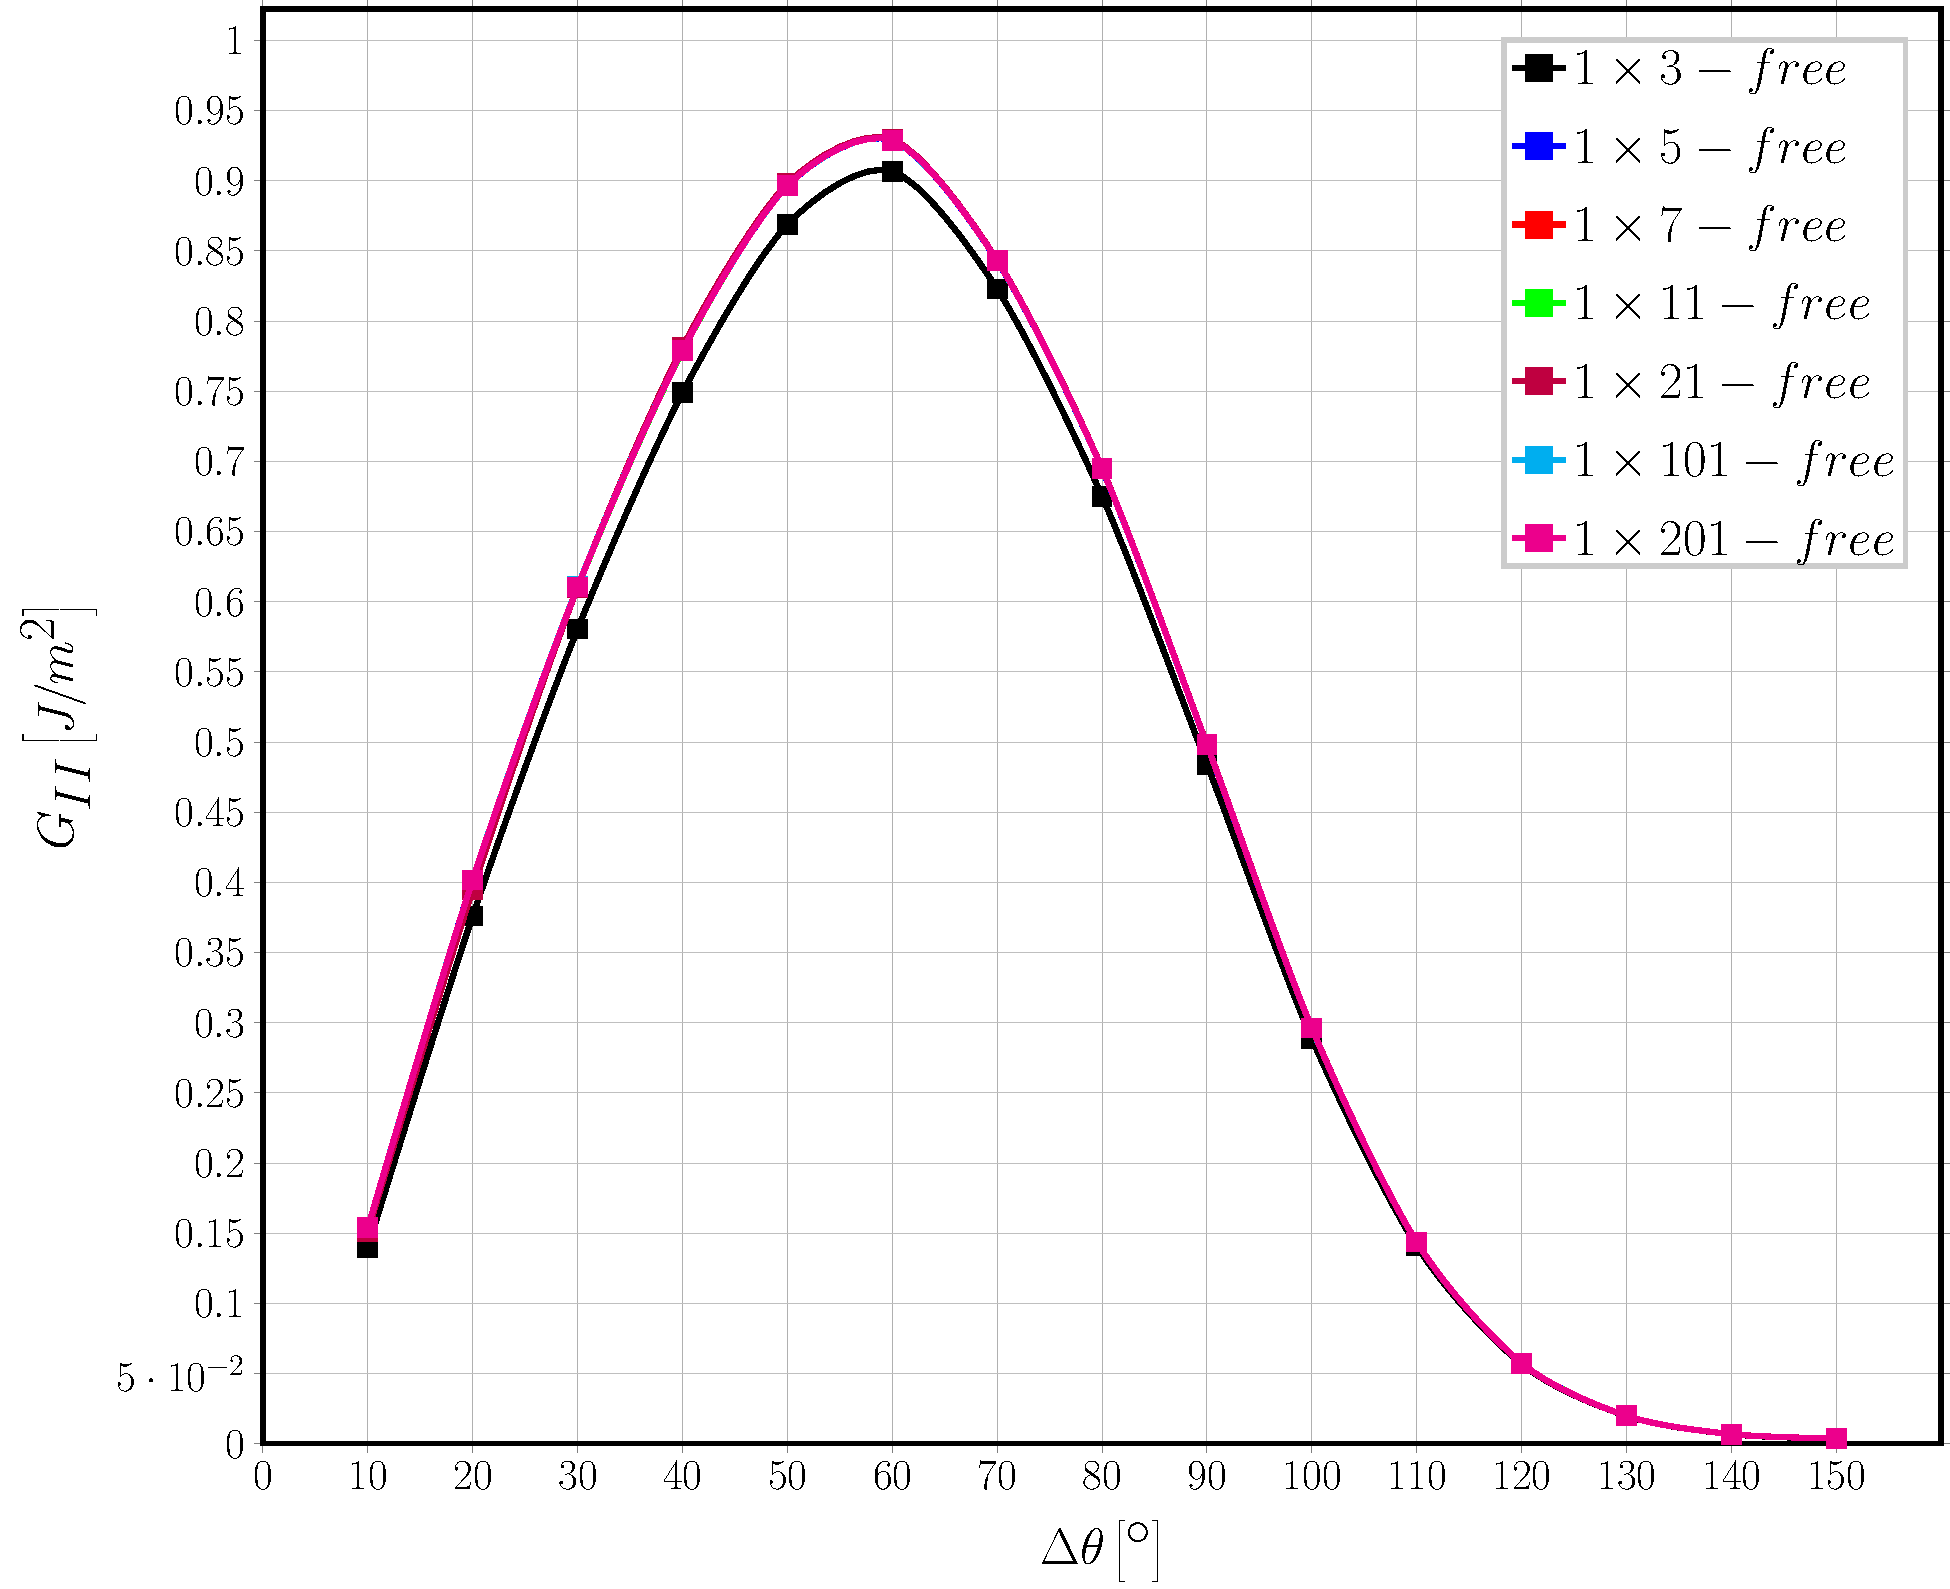
\includegraphics[width=\textwidth]{abovefibers-vf30-GII.pdf}
        \caption{$V_{f}=30\%$.}\label{subfig:abovefiber30MII}
    \end{subfigure} ~
    \begin{subfigure}[b]{0.45\textwidth}
        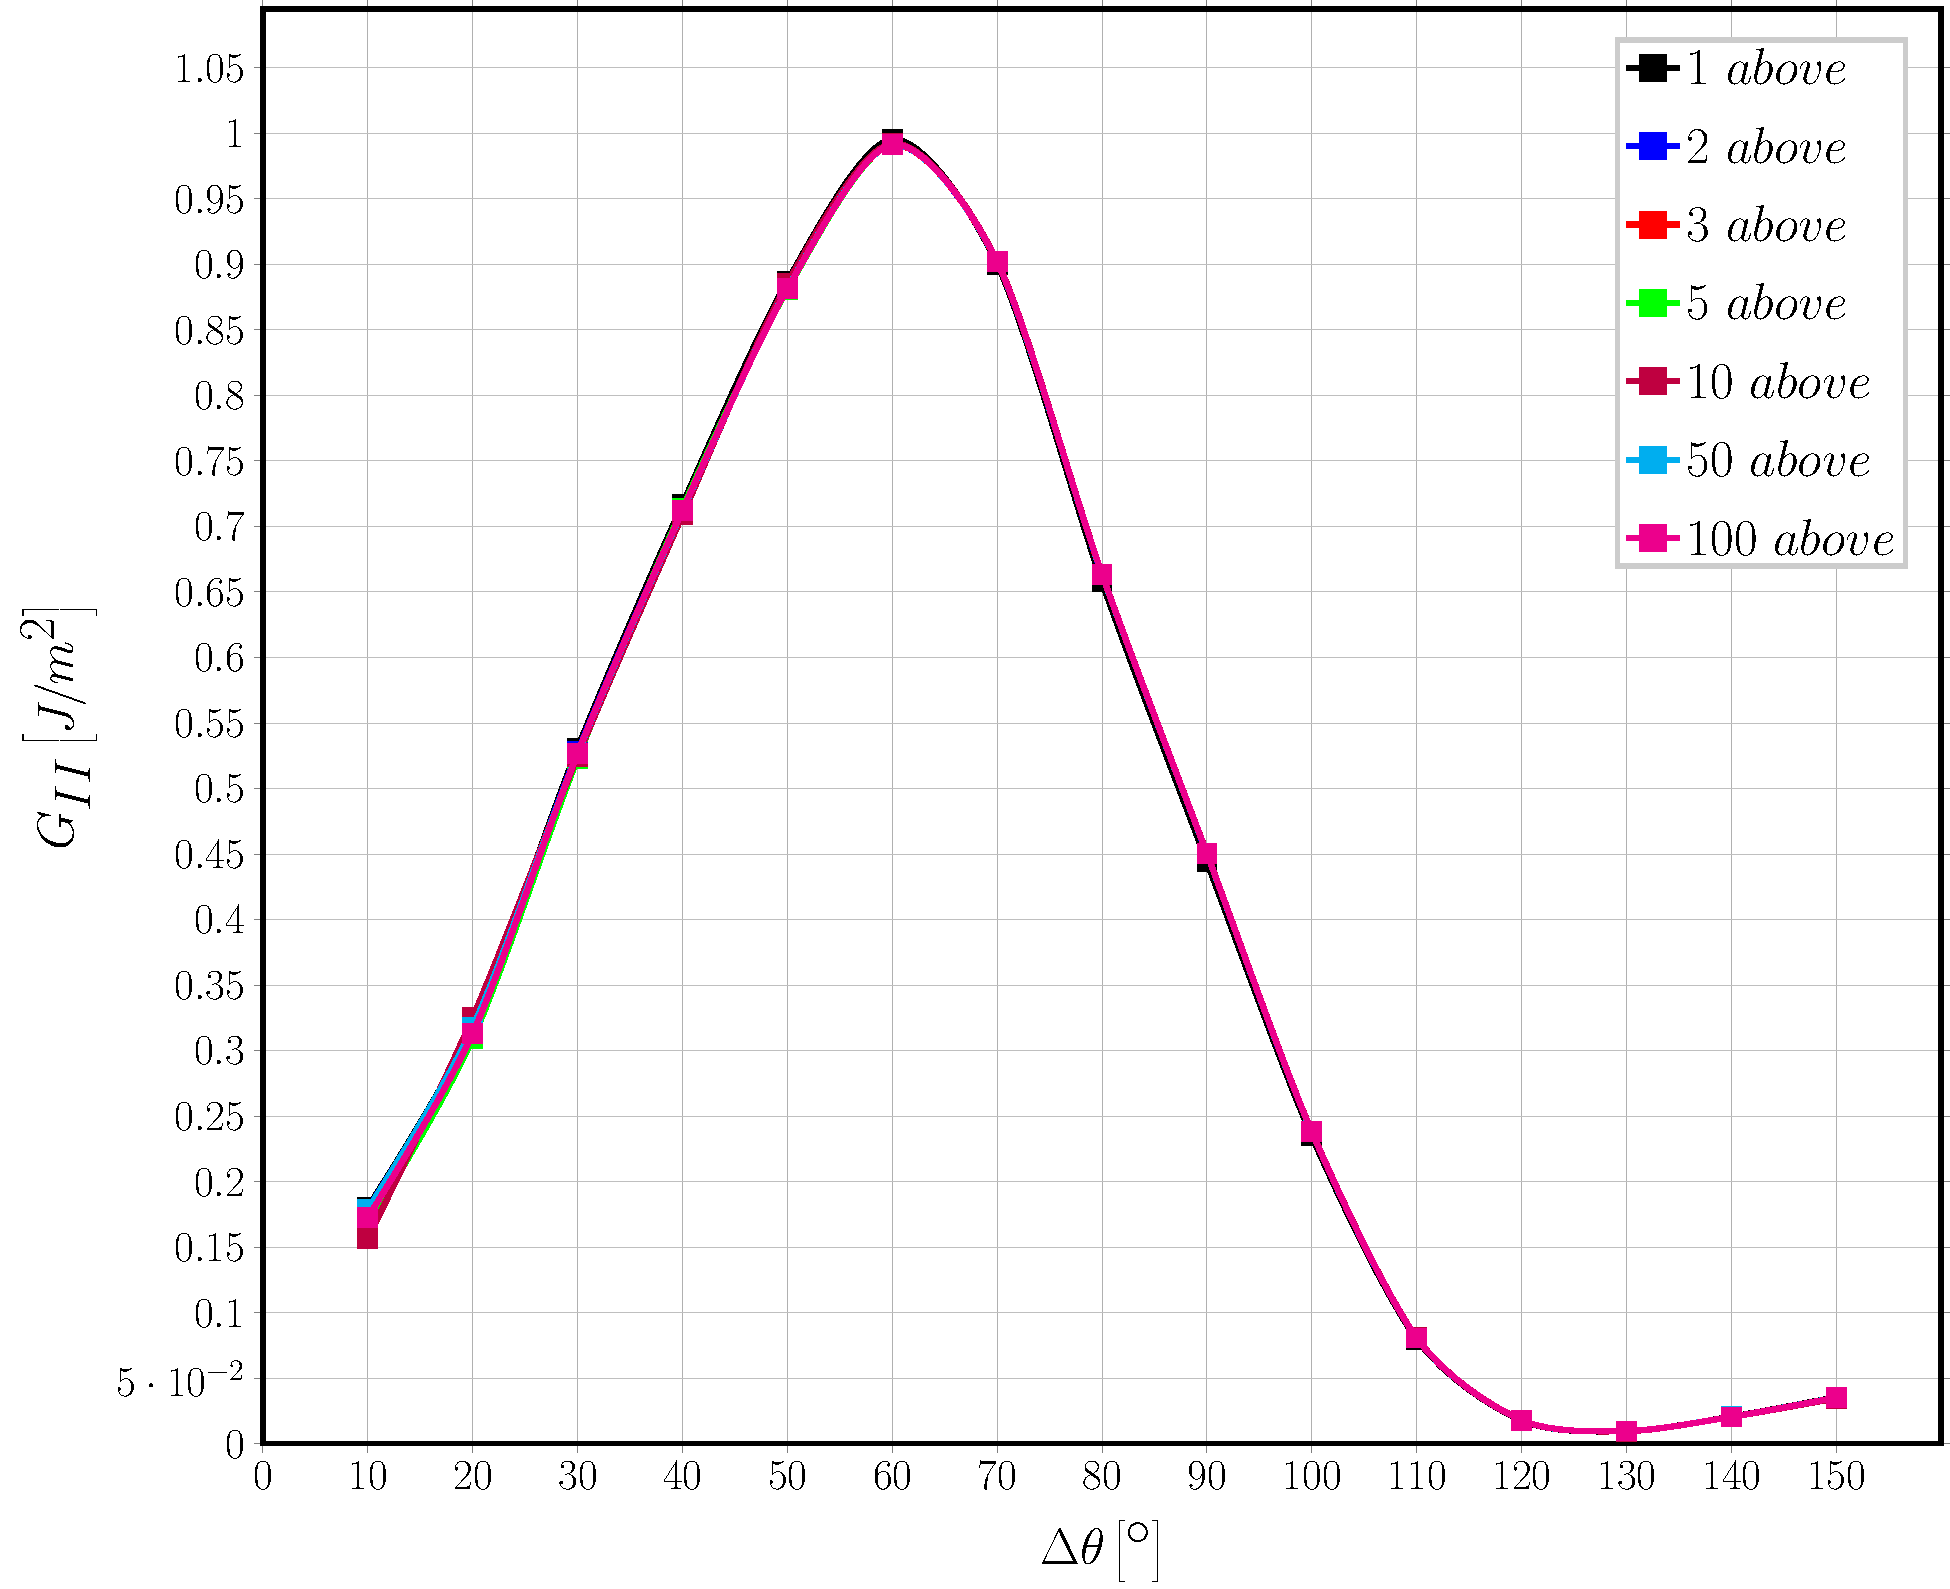
\includegraphics[width=\textwidth]{abovefibers-vf60-GII.pdf}
        \caption{$V_{f}=60\%$.}\label{subfig:abovefiber60MII}
    \end{subfigure}

\caption{Influence of layers of fully bonded fibers on debond's growth in Mode II ERR in a centrally located line of debonded fibers at different levels of fiber volume fraction $V_{f}$, subject to an applied transverse strain $\varepsilon_{x}$ of $1\%$.}\label{fig:abovefibersMII}
\end{figure}

The results of both Mode I and Mode II show that the introduction of an increasing number of fully bonded fiber rows doesn't change the ERR calculated at the crack tip (the convergence is very fast). A small effect, mostly on Mode I, of the number of bonded fiber rows can be observed at low fiber content (Figs.~\ref{subfig:abovefiber30MI} and~\ref{subfig:abovefiber30MII}), while for high fiber content the smaller model with only one fiber row above the partially debonded one is already representative.

\subsection{Interaction between debonds in central row of a UD composite with multiple rows of bonded fibers}\label{subsec:multrow}

The interaction of debonds appearing at regular intervals in the central row of fibers in UD composites with multiple rows of fibers is investigated using different combinations of horizontal debond spacing and the number of rows of bonded fibers across the thickness, corresponding to the models: $3\times 3-free$, $5\times 3-free$, $5\times 5-free$, $7\times 3-free$, $7\times 5-free$, $7\times 7-free$, $11\times 3-free$, $11\times 5-free$, $11\times 7-free$, $11\times 11-free$, $21\times 3-free$, $21\times 5-free$, $21\times 7-free$, $21\times 11-free$, $21\times 21-free$, $101\times 3-free$, $101\times 5-free$, $101\times 7-free$, $101\times 11-free$, $201\times 3-free$, $201\times 5-free$, $201\times 7-free$, $201\times 11-free$  (Fig.~\ref{subfig:thickply}).

\begin{figure}[!h]
\centering
    \begin{subfigure}[b]{0.475\textwidth}
        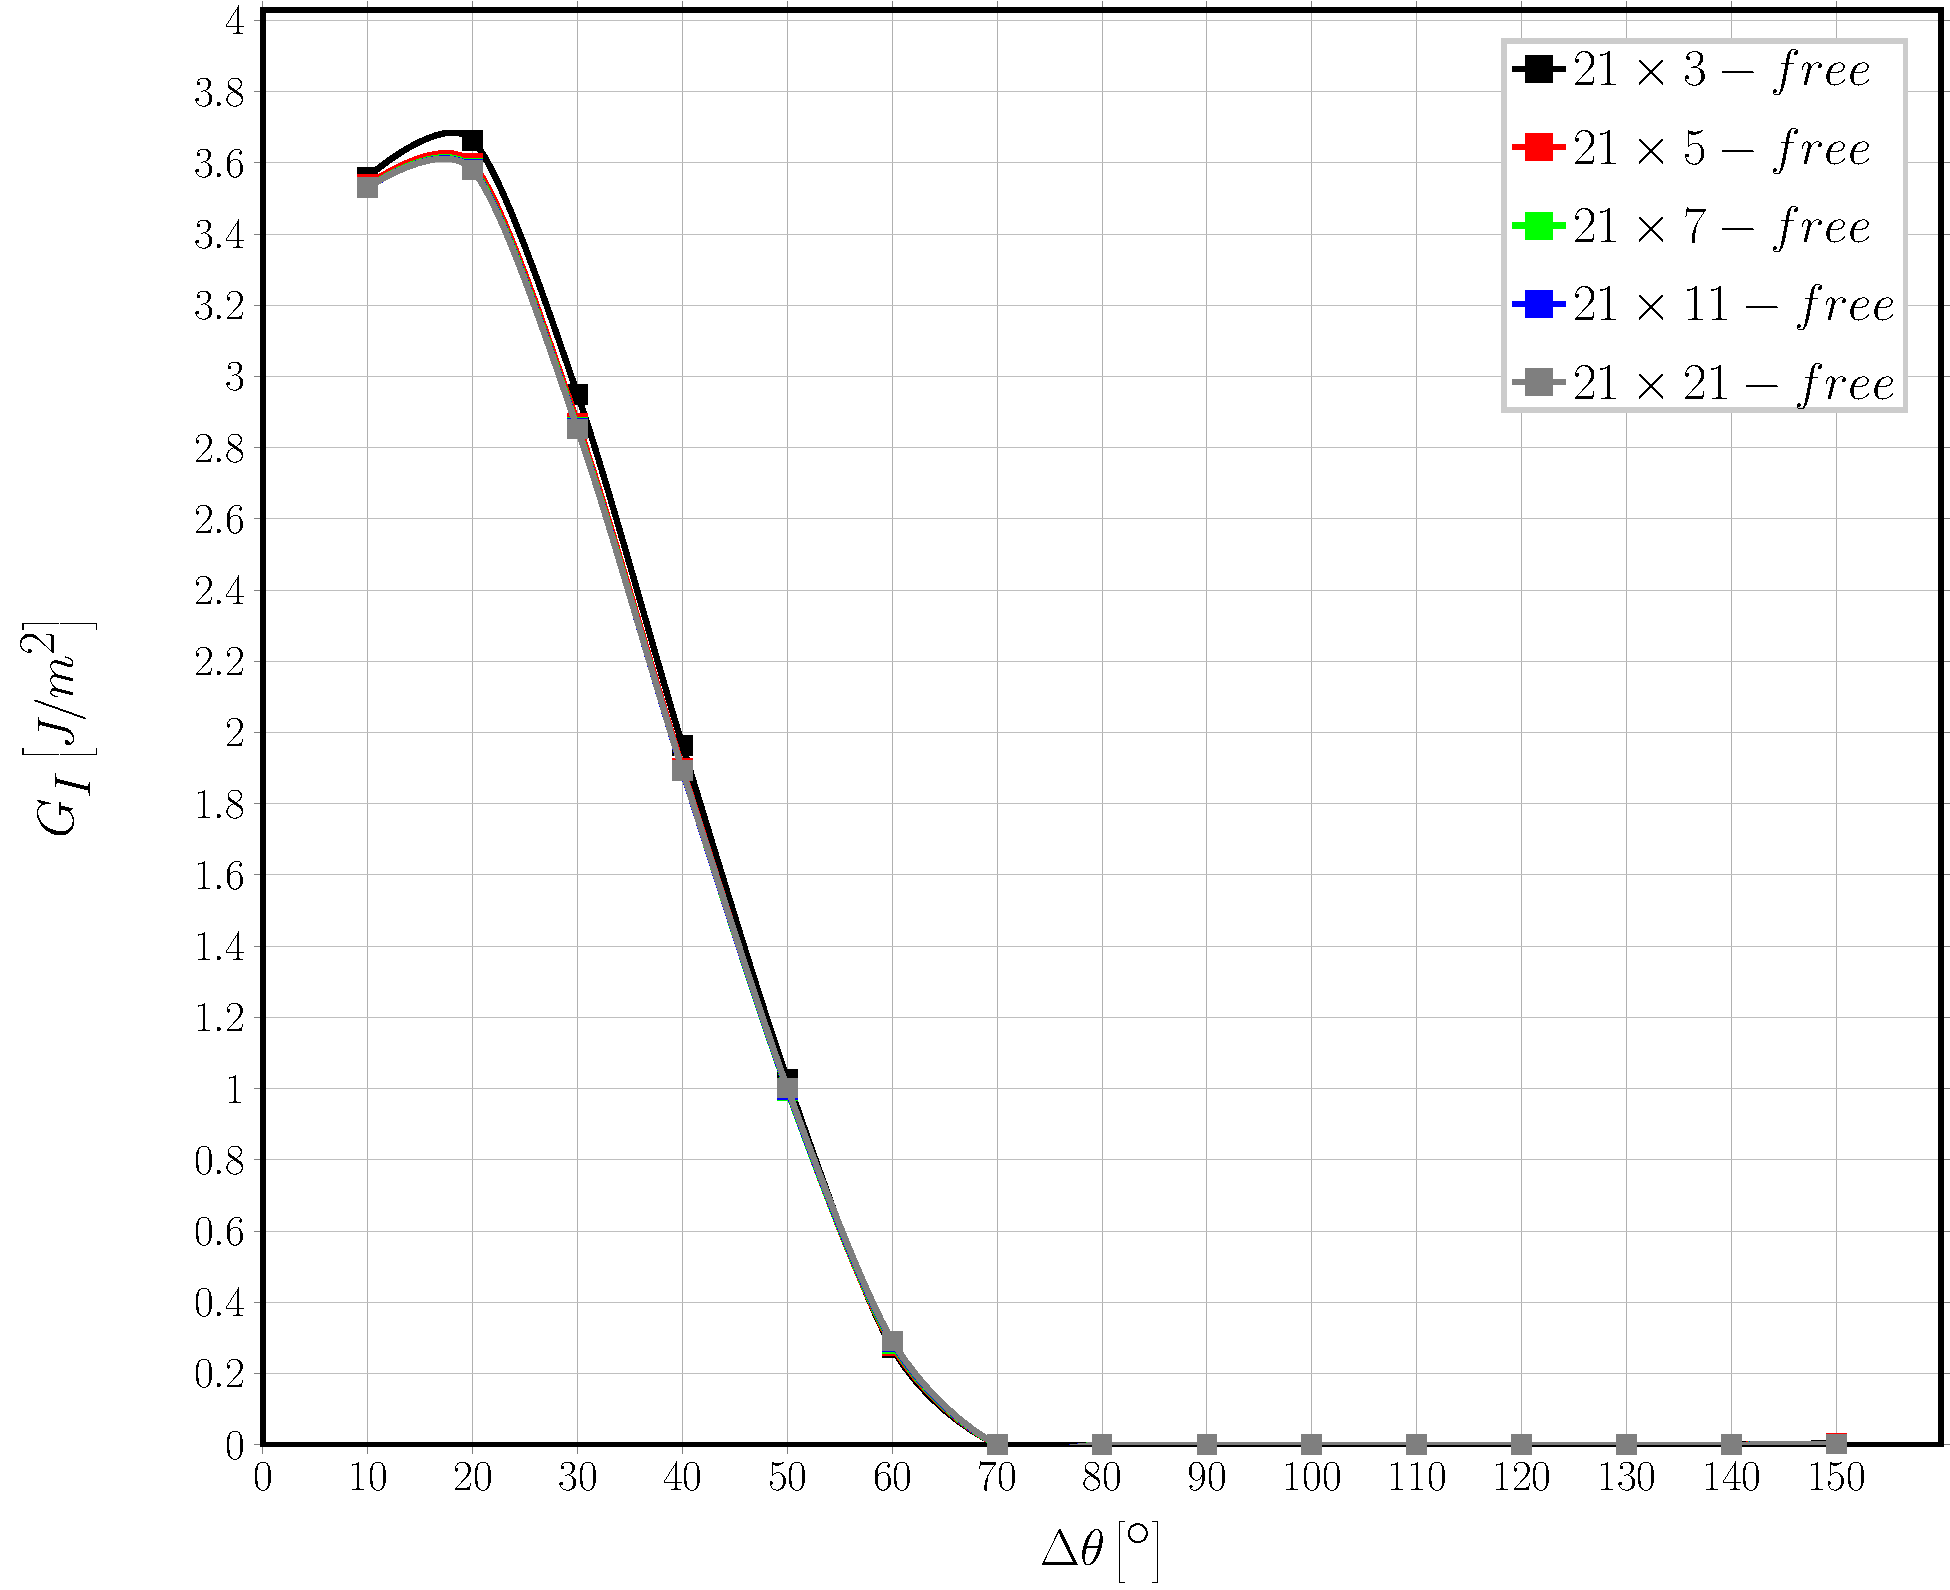
\includegraphics[width=\textwidth]{sideabovefibers-vf60-GI.pdf}
        \caption{$G_{I}$.}\label{subfig:sideabovefiber60MIsp}
    \end{subfigure} ~
    \begin{subfigure}[b]{0.475\textwidth}
        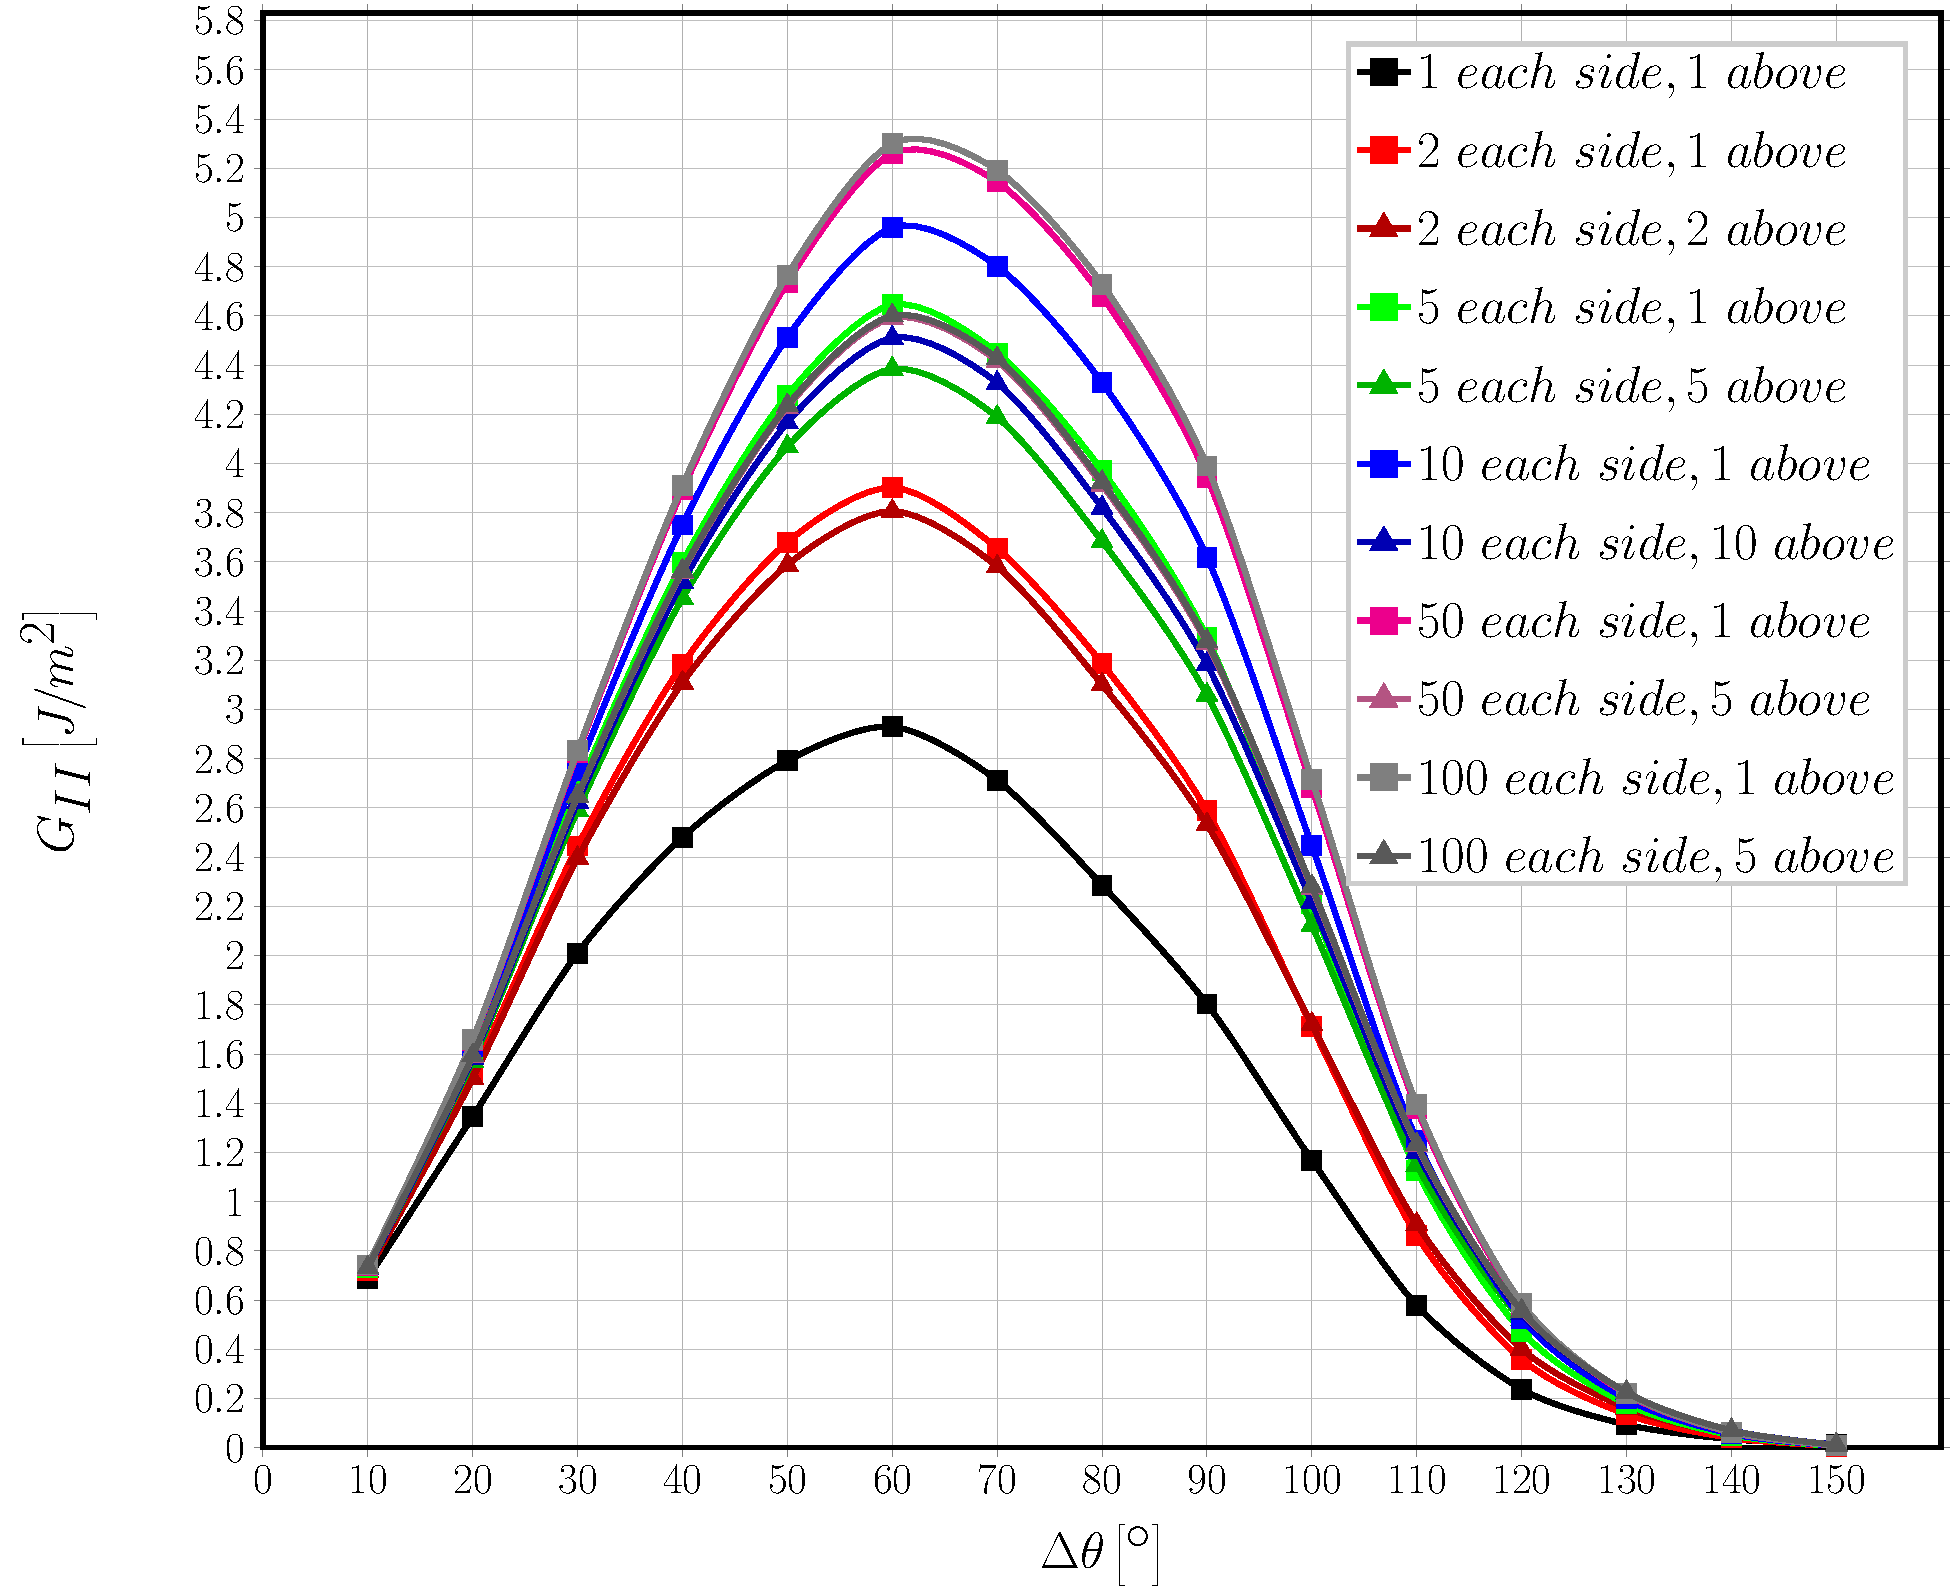
\includegraphics[width=\textwidth]{sideabovefibers-vf60-GII.pdf}
        \caption{$G_{II}$.}\label{subfig:sideabovefiber60MIIsp}
    \end{subfigure}

\caption{Effect on Mode I and Mode II ERR of the presence of an increasing number of rows of fully bonded fibers in UD composites with debonds appearing every $10^{th}$ fiber (model $21\times k-free$). $V_{f}=60\%$ and $\varepsilon_{x}=1\%$.}\label{fig:sideabovefibersspacingfixed}
\end{figure}

The results shown in Fig.~\ref{fig:sideabovefibersspacingfixed} confirm the observations discussed in Sec.~\ref{subsec:singlefiberud}: the presence of fully bonded fibers across the thickness has a restraining effect on the ERR, that counteracts the magnification due to an increasing number of fully bonded fibers in the horizontal direction. The interplay is further modulated by the fiber content. For Mode I, at high fiber content the contact zone onset starts at $70^{\circ}$ for $V_{f}=60\%$, delayed with respect to the low fiber content case of $60^{\circ}$. Comparing Fig.~\ref{fig:sideabovefibersspacingfixed} with Fig.~\ref{subfig:abovefiber60MI} and Fig.~\ref{subfig:abovefiber60MII}, it is furthermore possible to observe that the number of fully bonded fibers' rows necessary to reach convergence to a non-interacting solution in the vertical direction depends on the spacing of debonds in the central row. In Figures~\ref{subfig:abovefiber60MI} and~\ref{subfig:abovefiber60MII} the results for the $1\times 3-free$ model ($1$ row below and above) are already representative of all the other cases; in Fig.~\ref{fig:sideabovefibersspacingfixed} the solution doesn't change anymore once at least $3$ rows below and above the central one are present, when convergence in both $G_{I}$ and $G_{II}$ is required.

%Comparing with the results in Sec.~\ref{subsec:singlefiberud}, it can be observed how the presence of fully bonded fibers across the thickness has a restraining effect on the ERR, that counteracts the magnification due to an increasing number of fully bonded fibers in the horizontal direction. The interplay is further modulated by the fiber content. For Mode I, at low fiber content the contact zone onset starts at $60^{\circ}$, while it is delayed to debonds of $70^{\circ}$ for $V_{f}=60\%$. 

\begin{figure}[!h]
\centering
    \begin{subfigure}[b]{0.475\textwidth}
        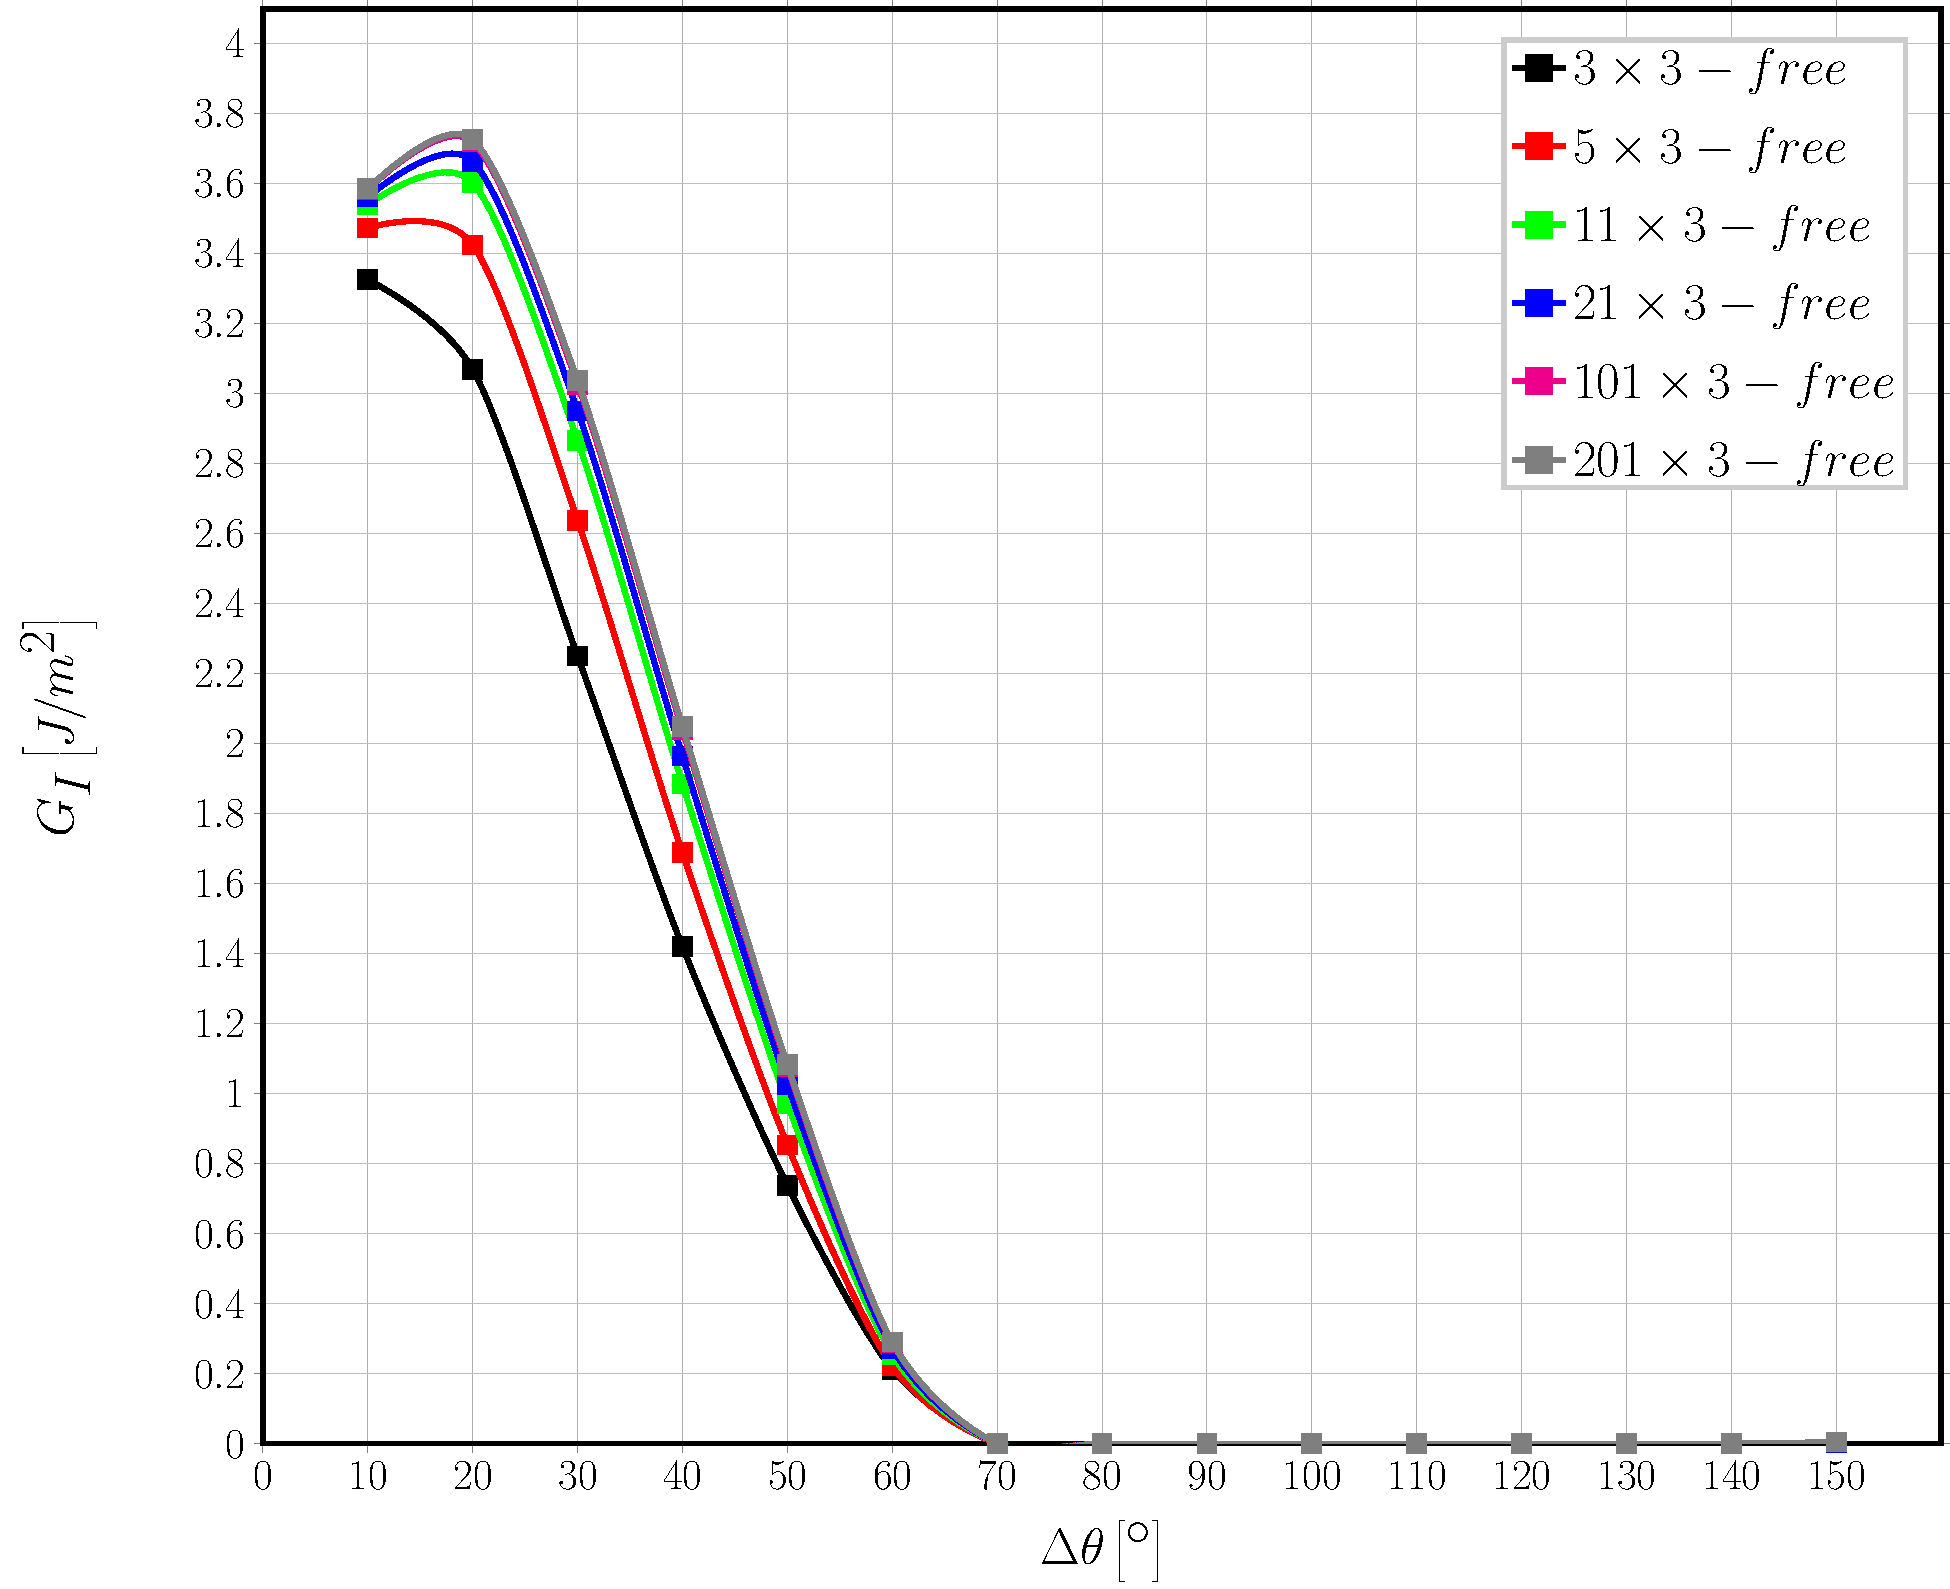
\includegraphics[width=\textwidth]{sideabovefibers-t3-vf60-GI.pdf}
        \caption{$k=3$, $G_{I}$.}\label{subfig:sideabovefiber60MIt3}
    \end{subfigure} ~
    \begin{subfigure}[b]{0.475\textwidth}
        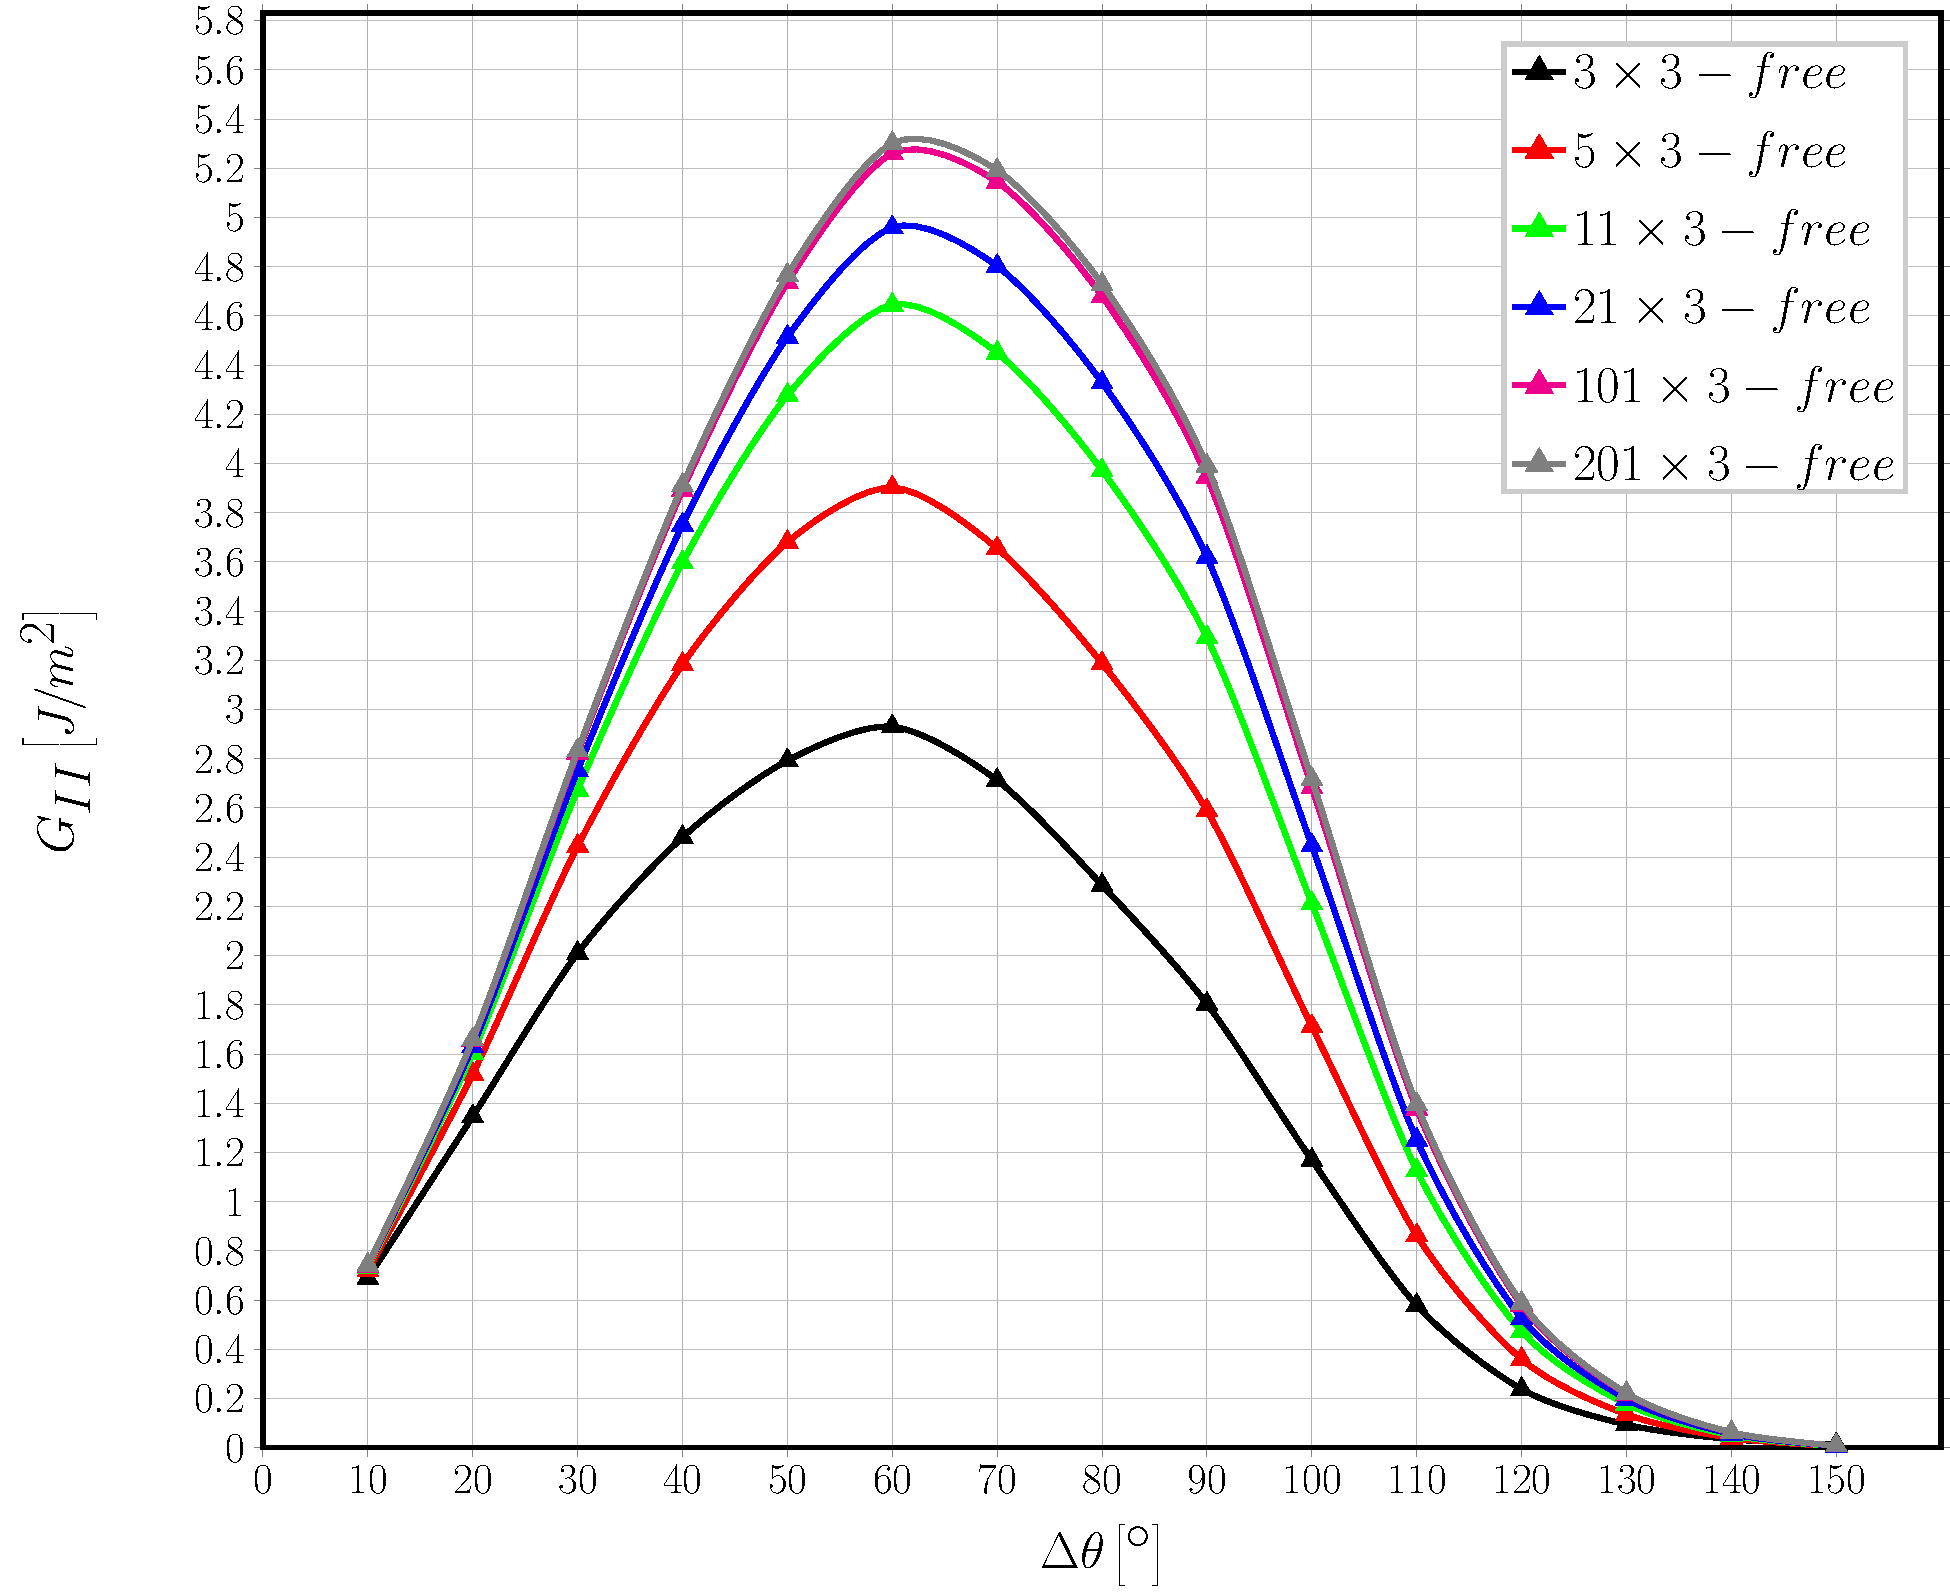
\includegraphics[width=\textwidth]{sideabovefibers-t3-vf60-GII.pdf}
        \caption{$k=3$, $G_{II}$.}\label{subfig:sideabovefiber60MIIt3}
    \end{subfigure}
    
    \begin{subfigure}[b]{0.475\textwidth}
        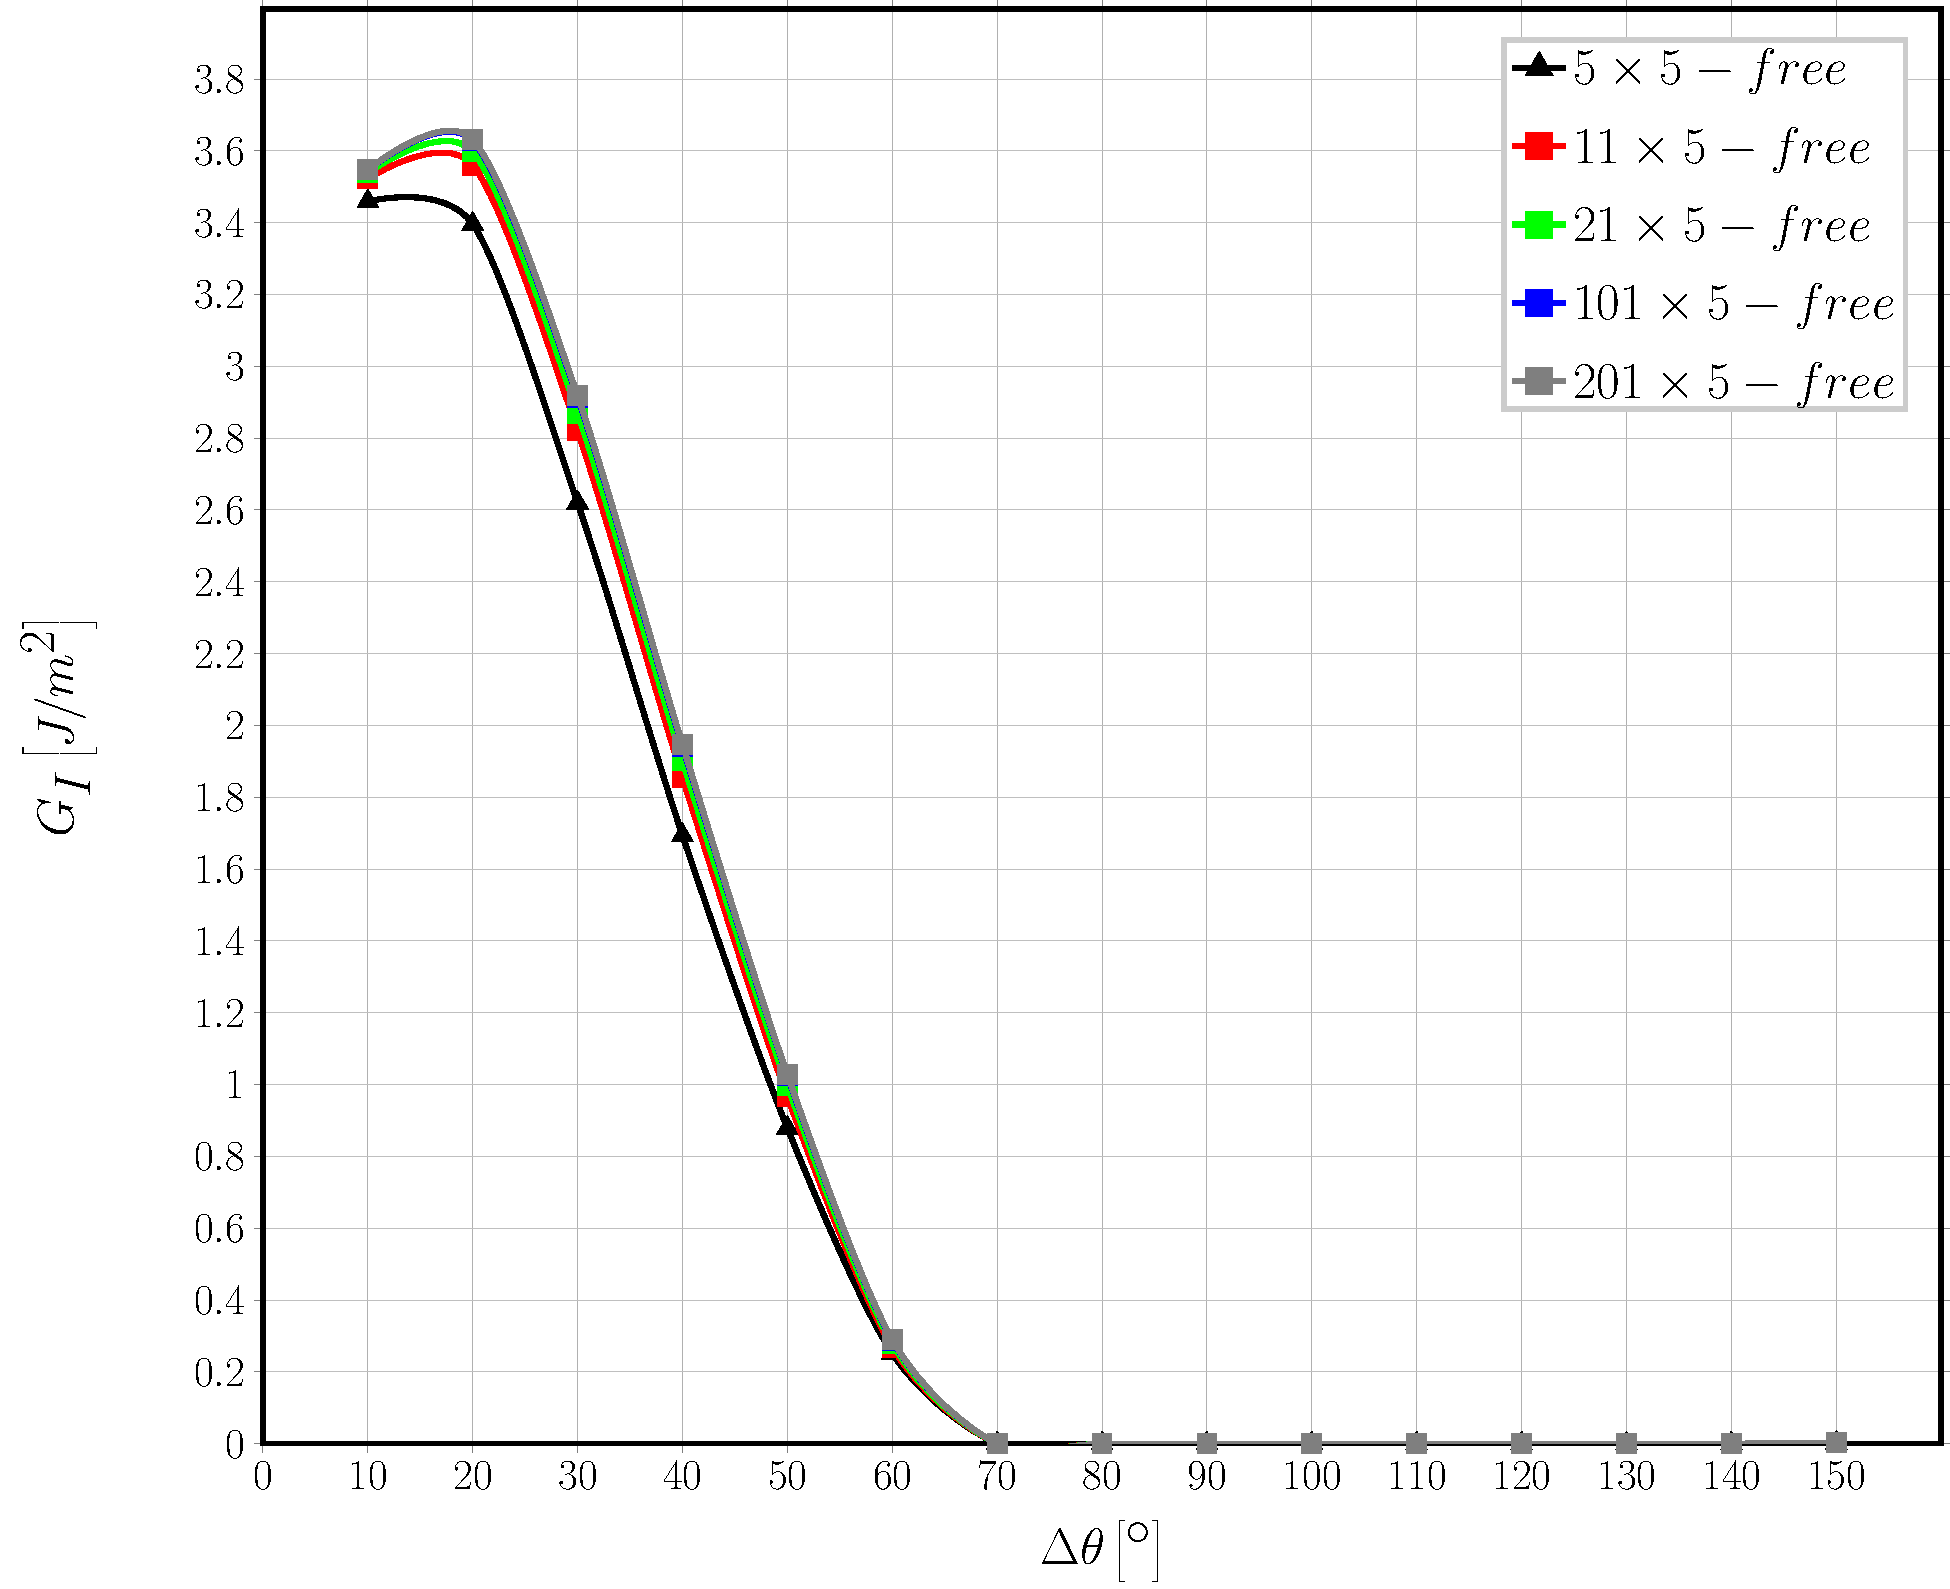
\includegraphics[width=\textwidth]{sideabovefibers-t5-vf60-GI.pdf}
        \caption{$k=5$, $G_{I}$.}\label{subfig:sideabovefiber60MIt5}
    \end{subfigure} ~
    \begin{subfigure}[b]{0.475\textwidth}
        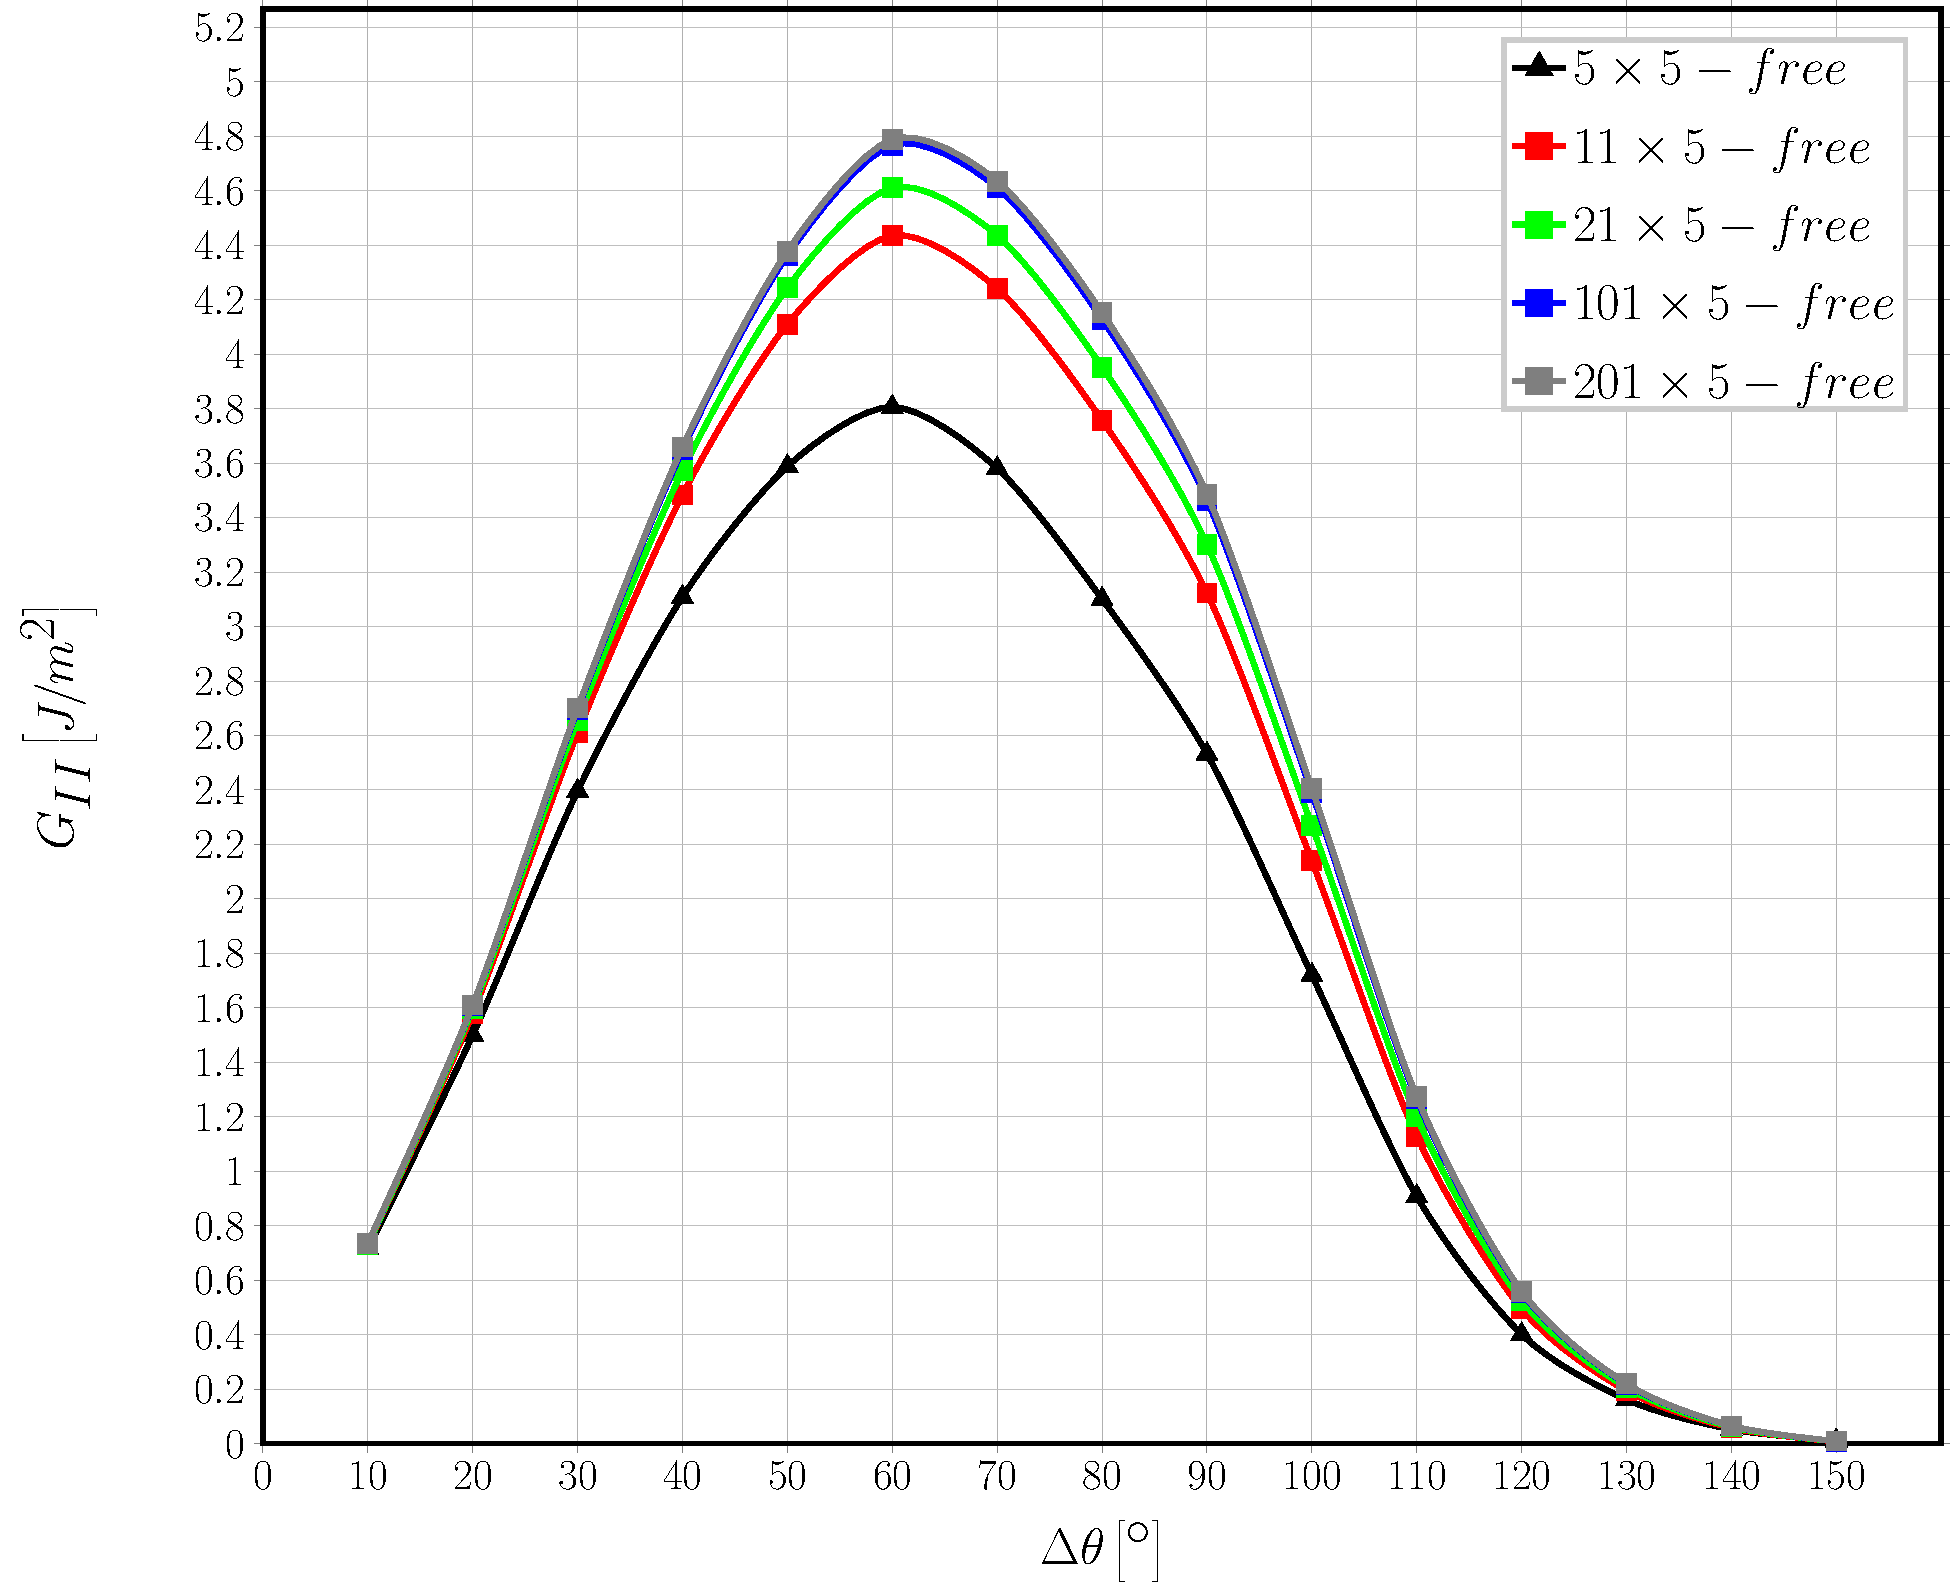
\includegraphics[width=\textwidth]{sideabovefibers-t5-vf60-GII.pdf}
        \caption{$k=5$, $G_{II}$.}\label{subfig:sideabovefiber60MIIt5}
    \end{subfigure}
    
    \begin{subfigure}[b]{0.475\textwidth}
        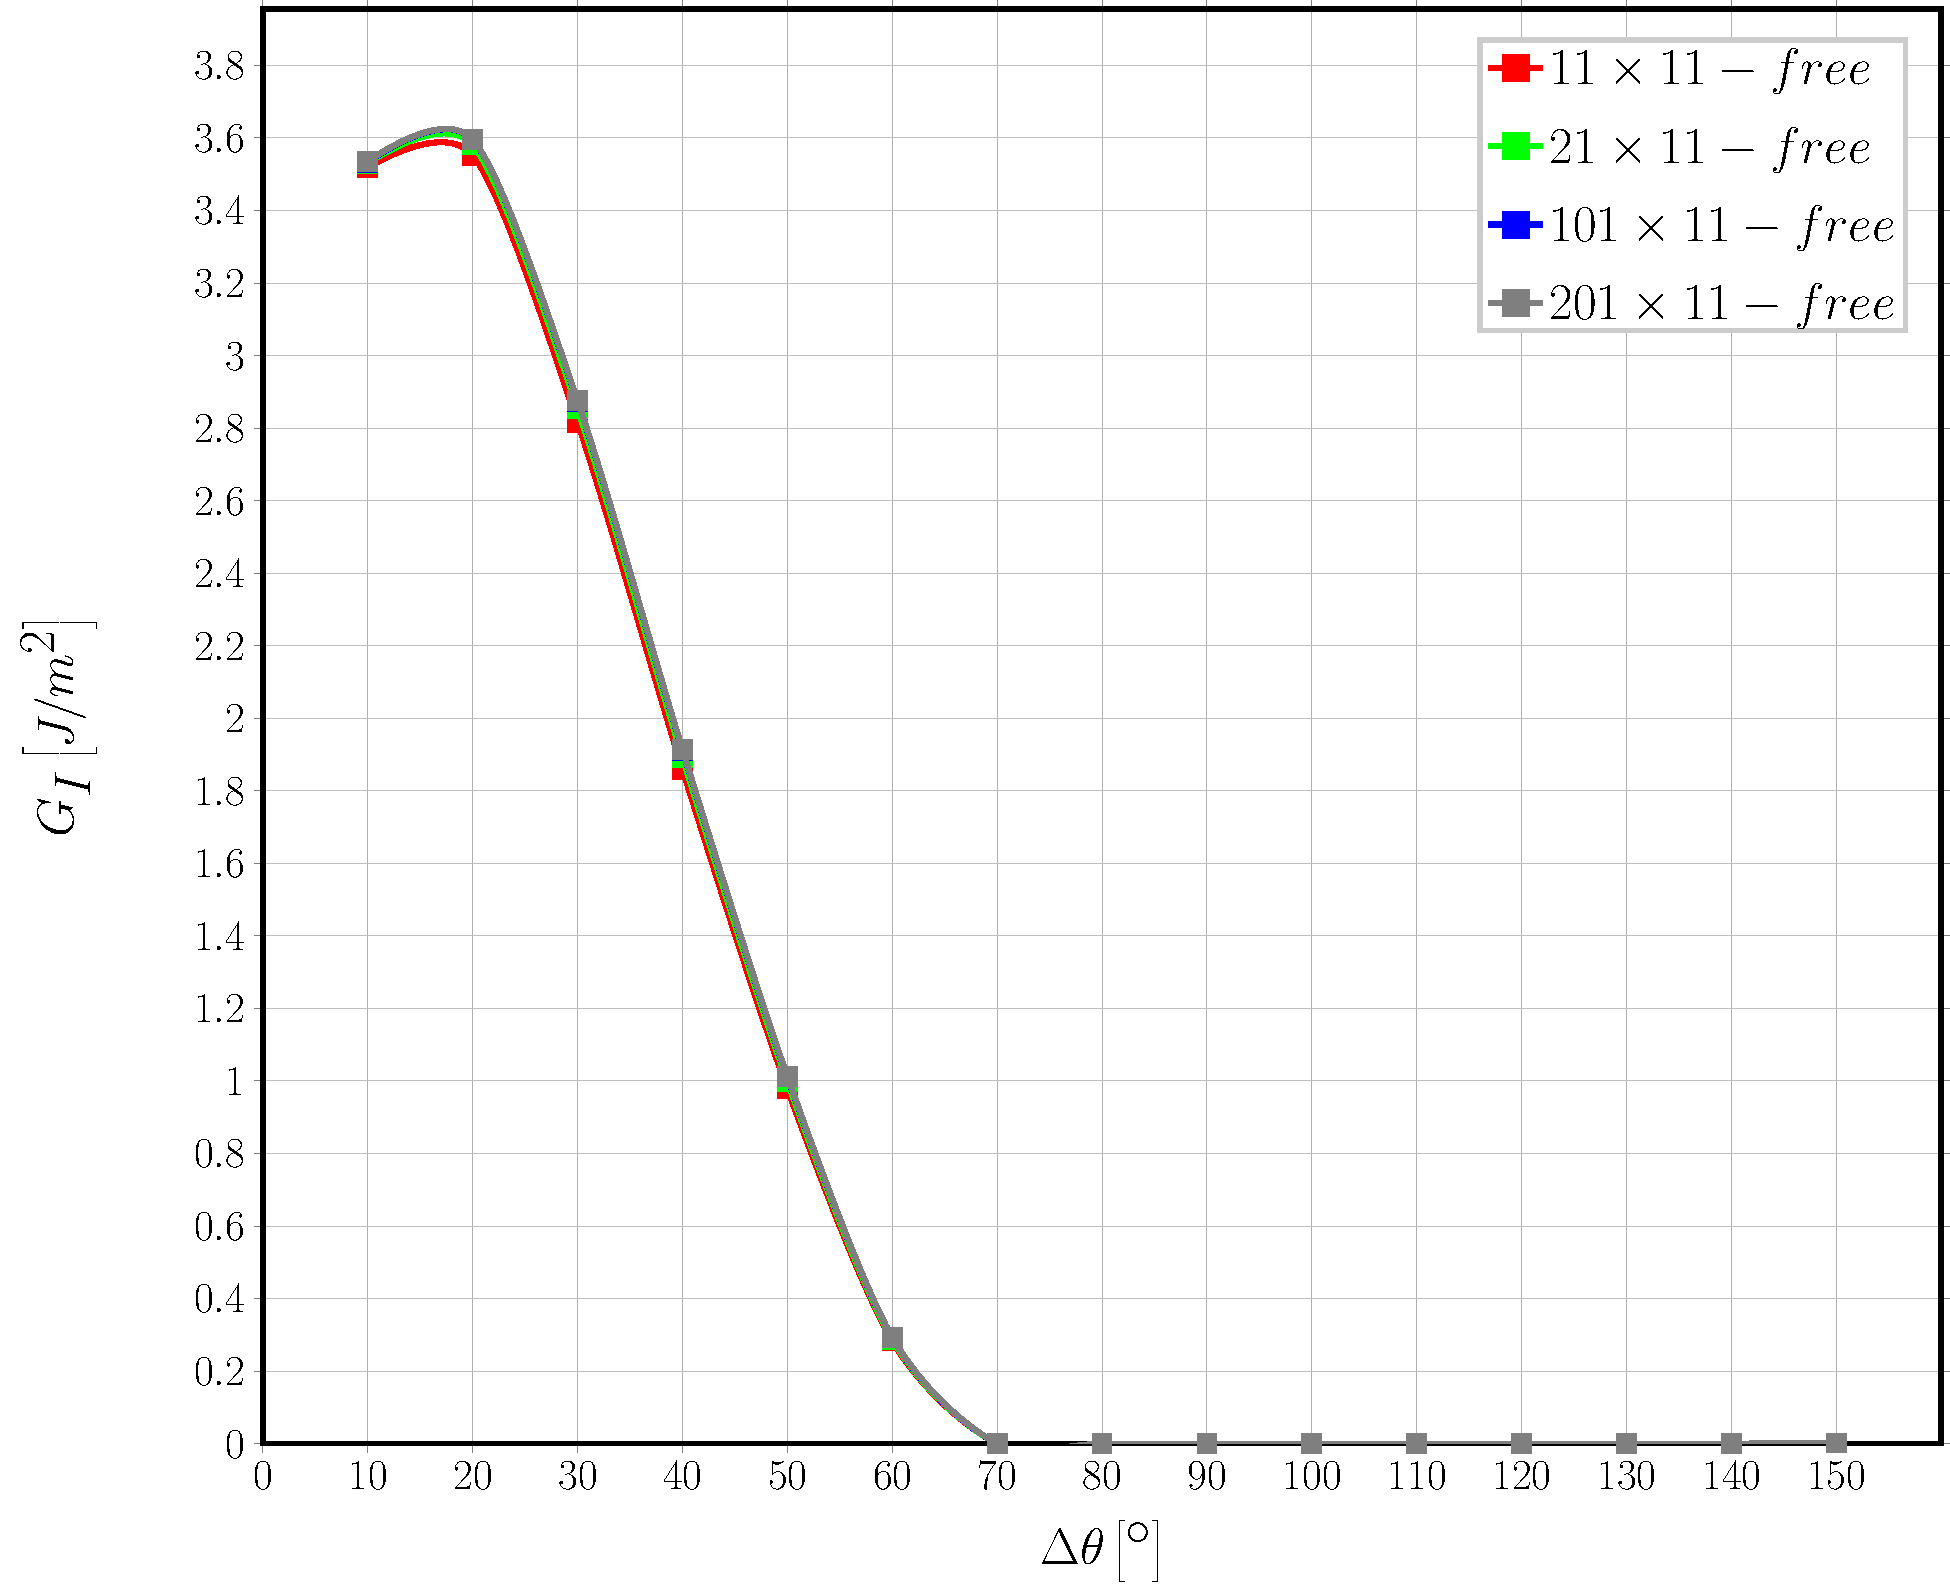
\includegraphics[width=\textwidth]{sideabovefibers-t11-vf60-GI.pdf}
        \caption{$k=11$, $G_{I}$.}\label{subfig:sideabovefiber60MIt11}
    \end{subfigure} ~
    \begin{subfigure}[b]{0.475\textwidth}
        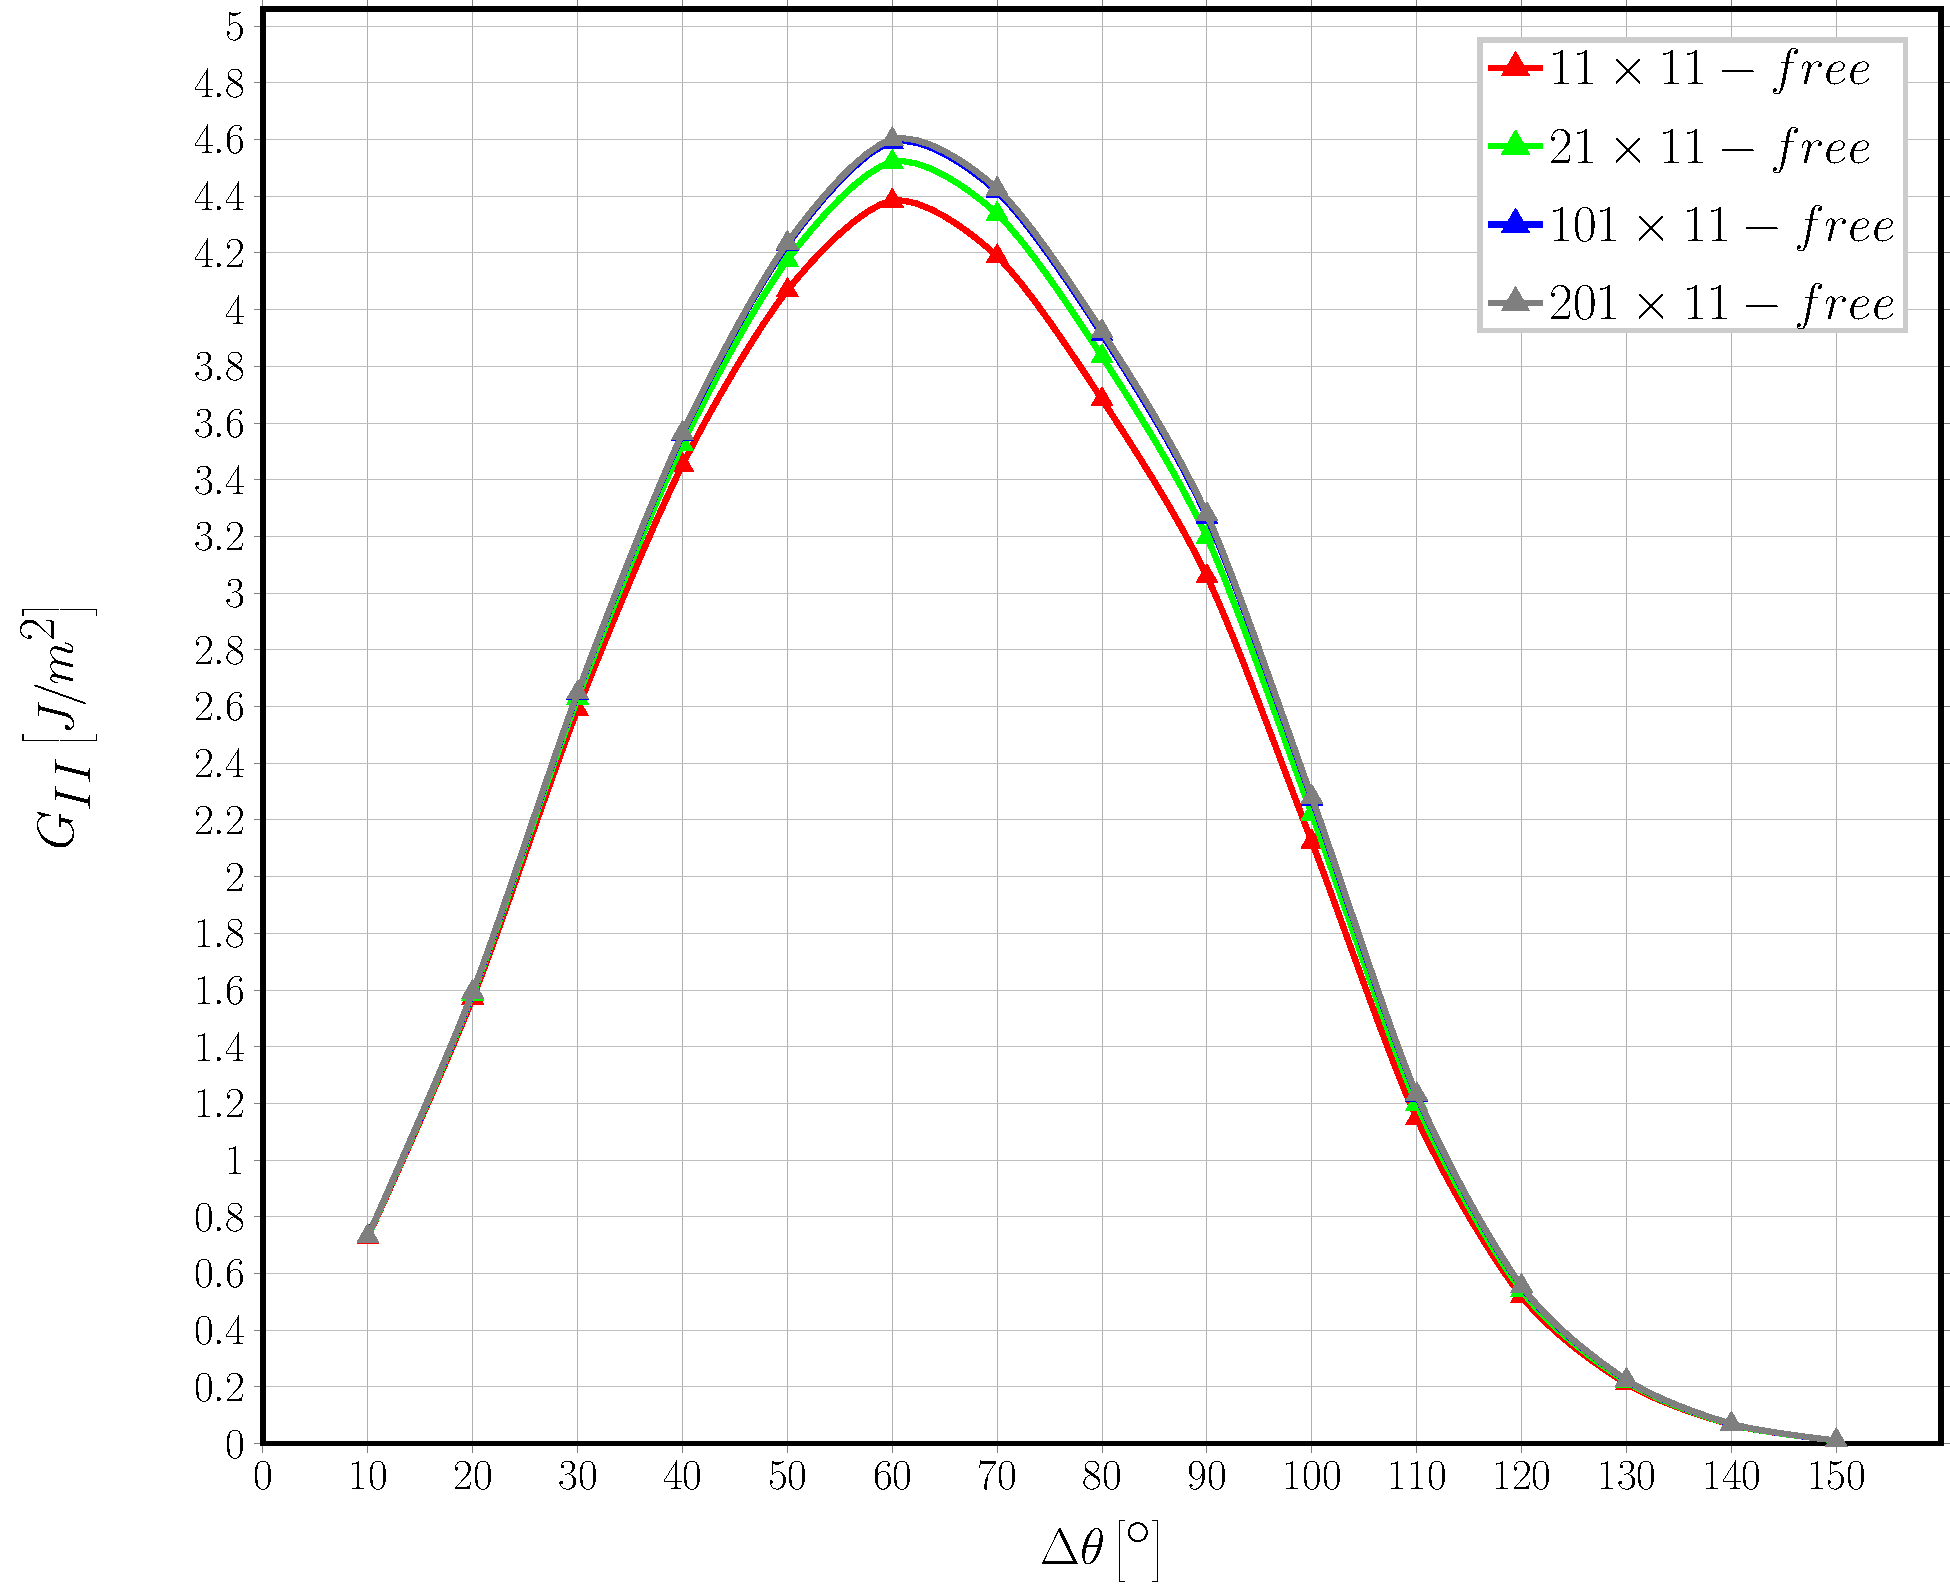
\includegraphics[width=\textwidth]{sideabovefibers-t11-vf60-GII.pdf}
        \caption{$k=11$, $G_{II}$.}\label{subfig:sideabovefiber60MIIt11}
    \end{subfigure}

\caption{Effect on Mode I and Mode II ERR of increasing the spacing between debonds appearing in the central row of fibers in a UD composite with a fixed number of rows across the thickness. $V_{f}=60\%$ and $\varepsilon_{x}=1\%$.}\label{fig:sideabovefibersthickfixed}
\end{figure}

The results in Fig.~\ref{fig:sideabovefibersthickfixed} show that the converse is as well as true: the characteristic distance (in terms of fully bonded fibers) between debonds for which a non-interactive solution is attained changes in relation to the thickness of the UD composite (defined by the number of rows in the vertical direction). Mode I appears to be far less sensitive than $G_{II}$ to the spacing of debonds in the horizontal direction when rows of fully bonded fibers are present above and below: in Fig.~\ref{subfig:sideabovefiber60MIt3} the increase in the peak value of $G_{I}$ is $\sim 8\%$ going from model $5\times 3-free$ to $201\times 3-free$, while $<5\%$ for larger spacings. In UDs of increased thickness, Figures~\ref{subfig:sideabovefiber60MIt5} and~\ref{subfig:sideabovefiber60MIt11}, the variation is further reduced. For Mode II, convergence to a non-interactive solution is reached with a spacing of $100$ fully bonded fibers for a UD with 3 rows of fibers across the thickness ($\frac{G_{II}^{201\times 3}\left(60^{\circ}\right)-G_{II}^{101\times 3}\left(60^{\circ}\right)}{G_{II}^{101\times 3}\left(60^{\circ}\right)}\sim0.7\%$), of $20$ fibers in a UD with 5 rows ($\frac{G_{II}^{101\times 5}\left(60^{\circ}\right)-G_{II}^{21\times 5}\left(60^{\circ}\right)}{G_{II}^{21\times 5}\left(60^{\circ}\right)}\sim4.3\%$) and of $10$ fibers in a UD with 11 rows ($\frac{G_{II}^{21\times 11}\left(60^{\circ}\right)-G_{II}^{11\times 11}\left(60^{\circ}\right)}{G_{II}^{11\times 11}\left(60^{\circ}\right)}\sim3.4\%$).

%It seems to be apparent that the interaction of debonds is strongly affected by the presence of fully bonded fiber between them: the further apart debonds in the central row are, the higher the Energy Release Rate. The presence of layers of fully bonded fibers has instead a suppressing effect and there exists a limit value of layers after which no sizeable change is measurable. Such limit value seems however to depend on the spacing of debonds in the horizontal direction. Increasing the fiber content leads in general to more drastic changes in the ERR.
%
%Convergence can also be observed: at $30\%$ fiber volume fraction, the $5\times 2-free$ model can already be considered representative of further spaced debonds in arbitrarily thick UDs; at $60\%$, the $21\times 2-free$ model can be considered representative of laminates with 3 layers of fibers and the $11\times 6-free$ of thicker UDs. A less definite situation characterizes instead Mode II. An increase in the value of ERR can be observed for any additional fully bonded fiber present in the horizontal direction, while a change due to the number of fibers across the thickness can be observed only between $1$ and $>1$.

\subsection{Comparison with the single fiber model with equivalent boundary conditions}

The single fiber RUC ($1\times 1-free$ or $1\times 1-coupling$) corresponds to the most damaged state of the composite, i.e. the state in which all fibers have debonds. The $1\times 1-free$ model represents an ultra-thin UD composite with a single row of partially debonded fibers. The $1\times 1-coupling$ model, where the displacement coupling is used to enforce periodic boundary conditions, represents an infinite composite.\\
The comparison of the $1\times 1-free$  model with one row multi-fiber models $n\times 1-free$ in Figure~\ref{fig:comparisonfree} show that the former provides in general the lowest value of the ERR (the highest crack shielding case) which is consistent with the trends observed in Section~\ref{subsec:singlefiberud}.

\begin{figure}[!h]
\centering
    \begin{subfigure}[b]{0.475\textwidth}
        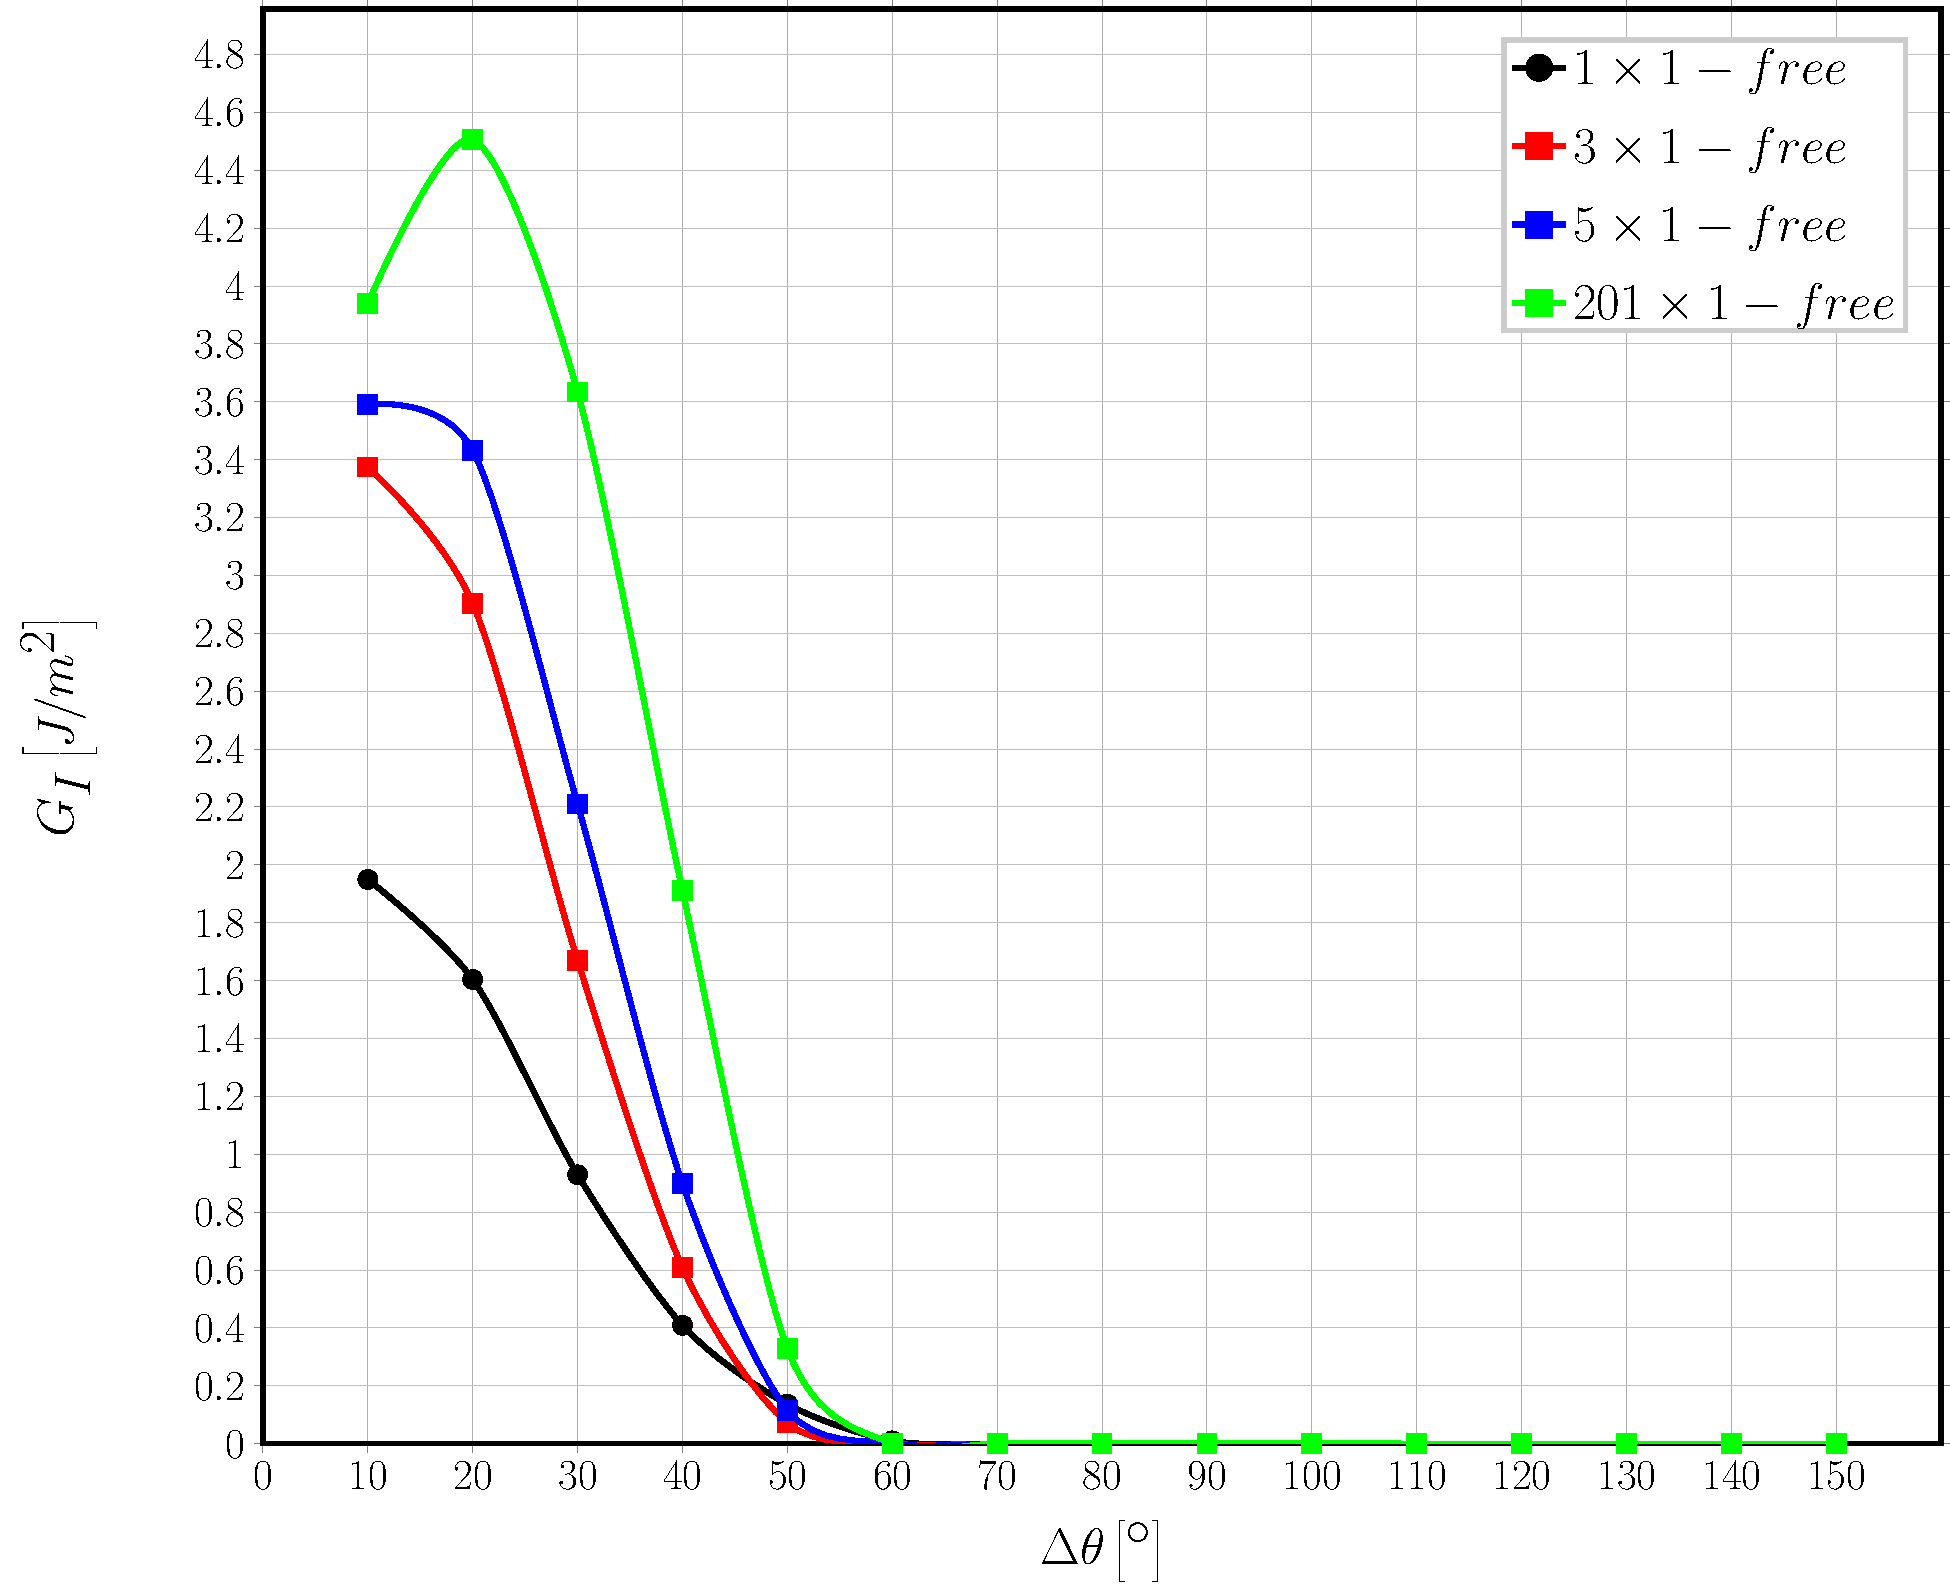
\includegraphics[width=\textwidth]{comparefreesidefibers-vf60-GI.pdf}
        \caption{$G_{I}$.}\label{subfig:comparisonfree60MI}
    \end{subfigure} ~
    \begin{subfigure}[b]{0.475\textwidth}
        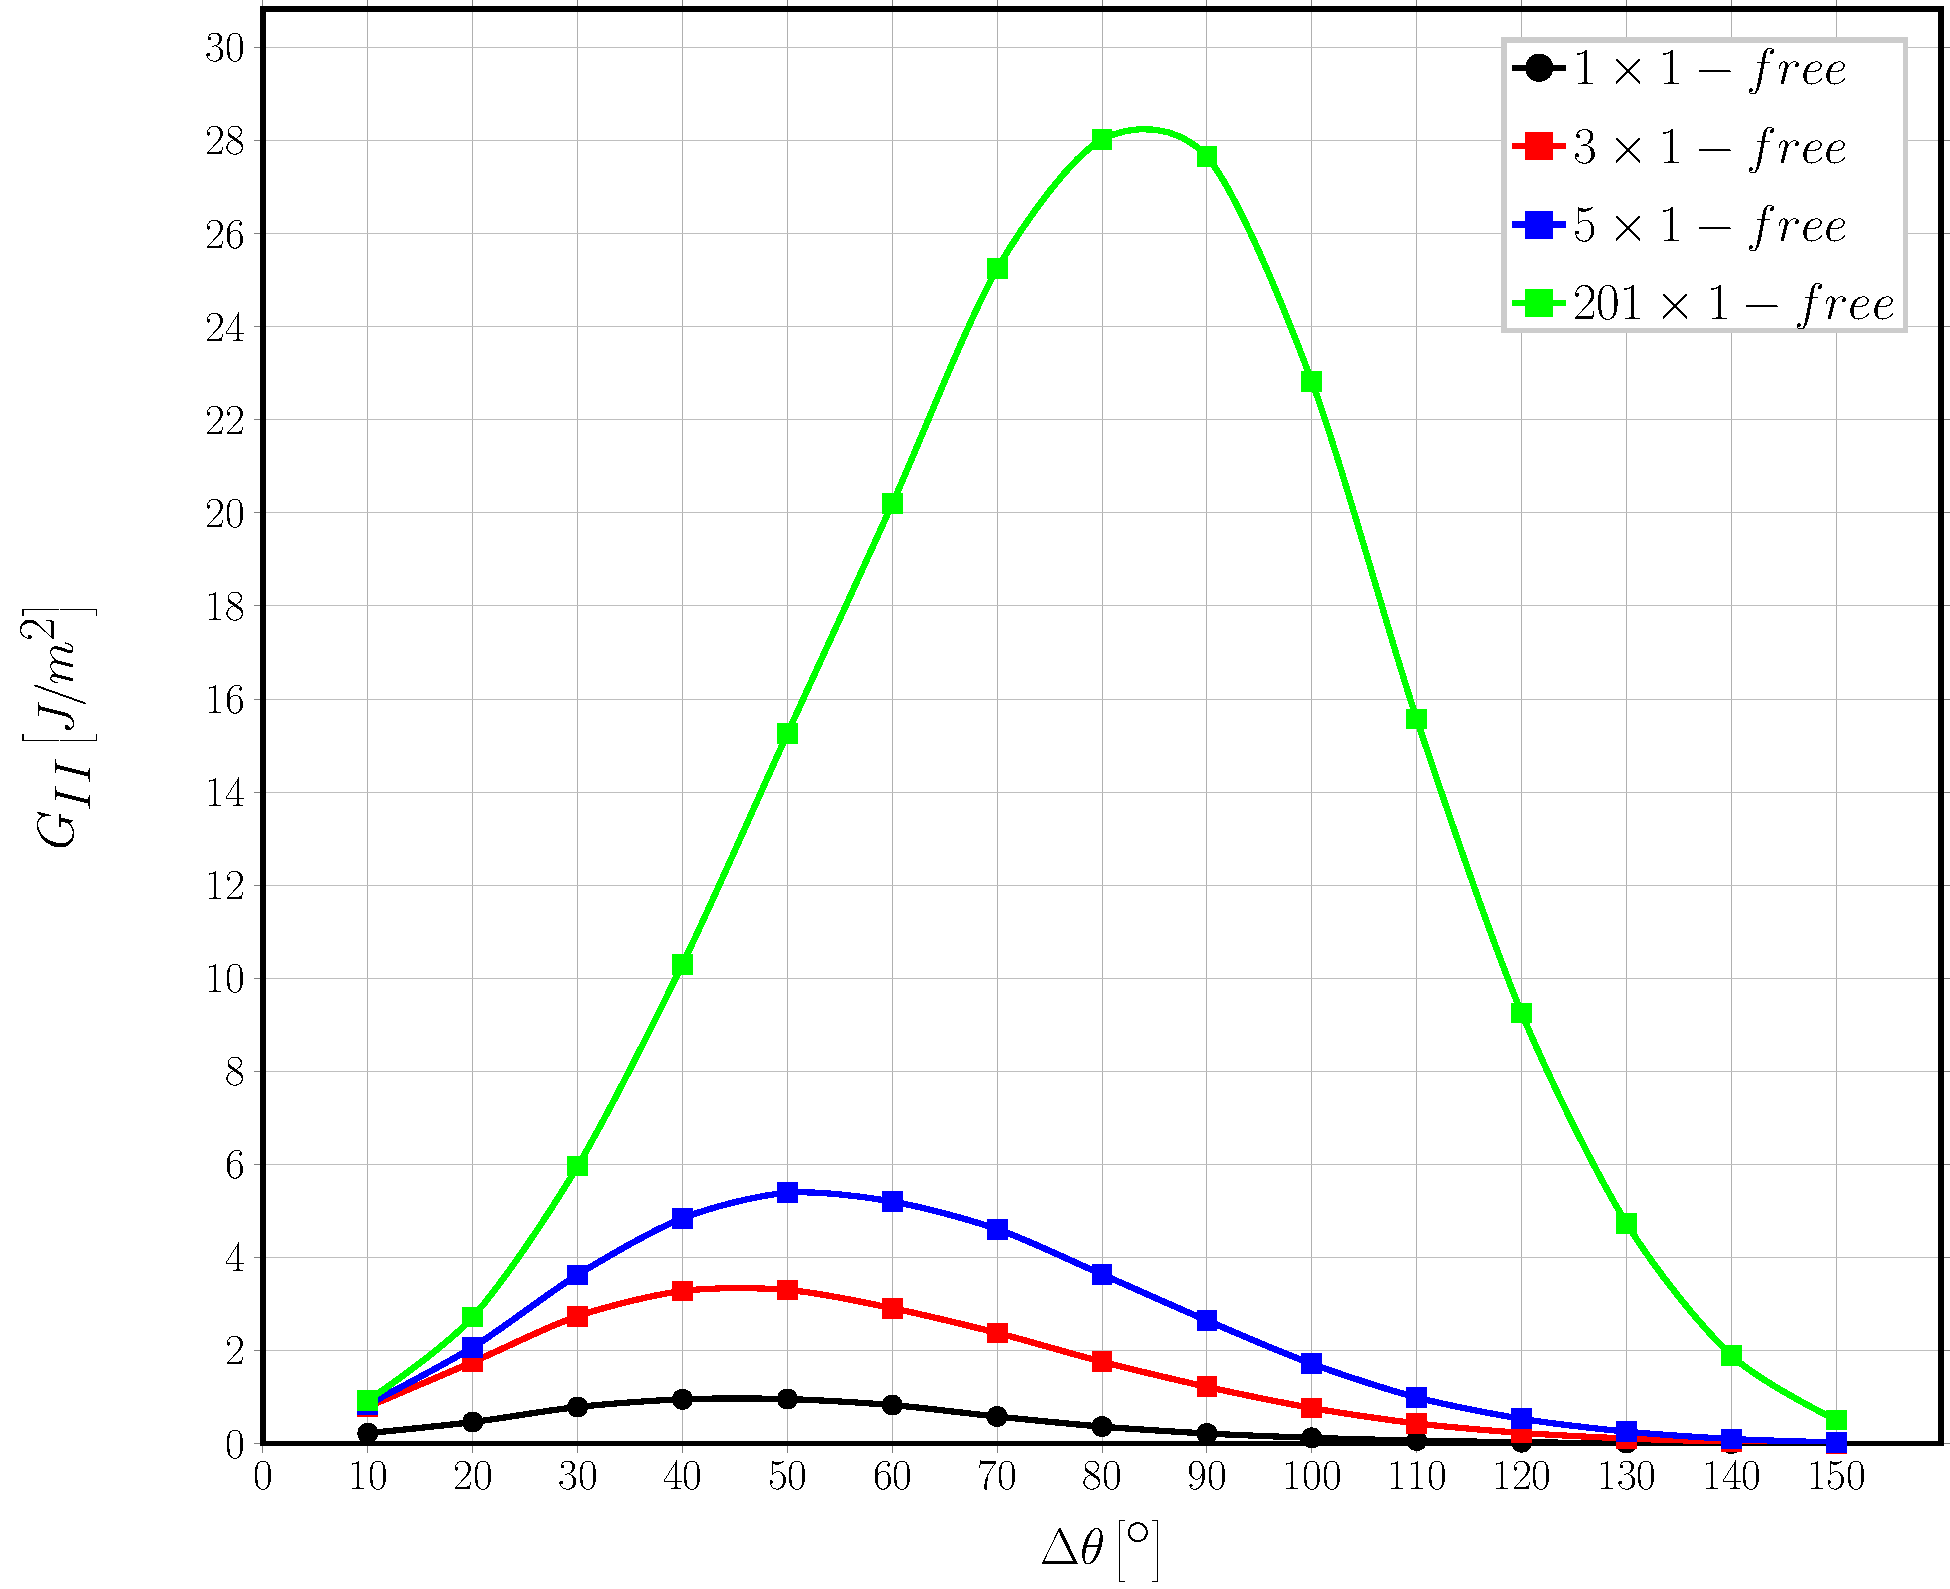
\includegraphics[width=\textwidth]{comparefreesidefibers-vf60-GII.pdf}
        \caption{$G_{II}$.}\label{subfig:comparisonfree60MII}
    \end{subfigure}

\caption{Comparison of the ERR between the single fiber model with free upper boundary and the multiple fibers model with fibers only on the side. $V_{f}=60\%$ and $\varepsilon_{x}=1\%$.}\label{fig:comparisonfree}
\end{figure}

The $1\times 1-coupling$ model is compared with $1\times 3-free$ and $1\times 201-free$ models in Fig.~\ref{fig:comparisoncoupling}. In all three models the distance between debonds in the $x$-direction is the same and the difference is in the vertical direction. The $1\times 1-coupling$ model describes the interaction between debonds in different rows of debonded fibers whereas the $1\times k-free$ models describe the effect of the proximity of the composite's free surface. The Mode I ERR in the $1\times 3-free$ model and in the $1\times 1-coupling$ model is very similar, which leads to a rather surprising conclusion. In both models we have, on the top of the central one, a large amount of fibers (bonded in one case and debonded in the other case). It appears that the effect of bonded and debonded fibers on the central debond is the same. This implies that the interaction between debonded fibers in elements placed on top of each other is small. The volume fraction effect is much smaller in high fiber content composites of this type.

\begin{figure}[!h]
\centering
    \begin{subfigure}[b]{0.475\textwidth}
        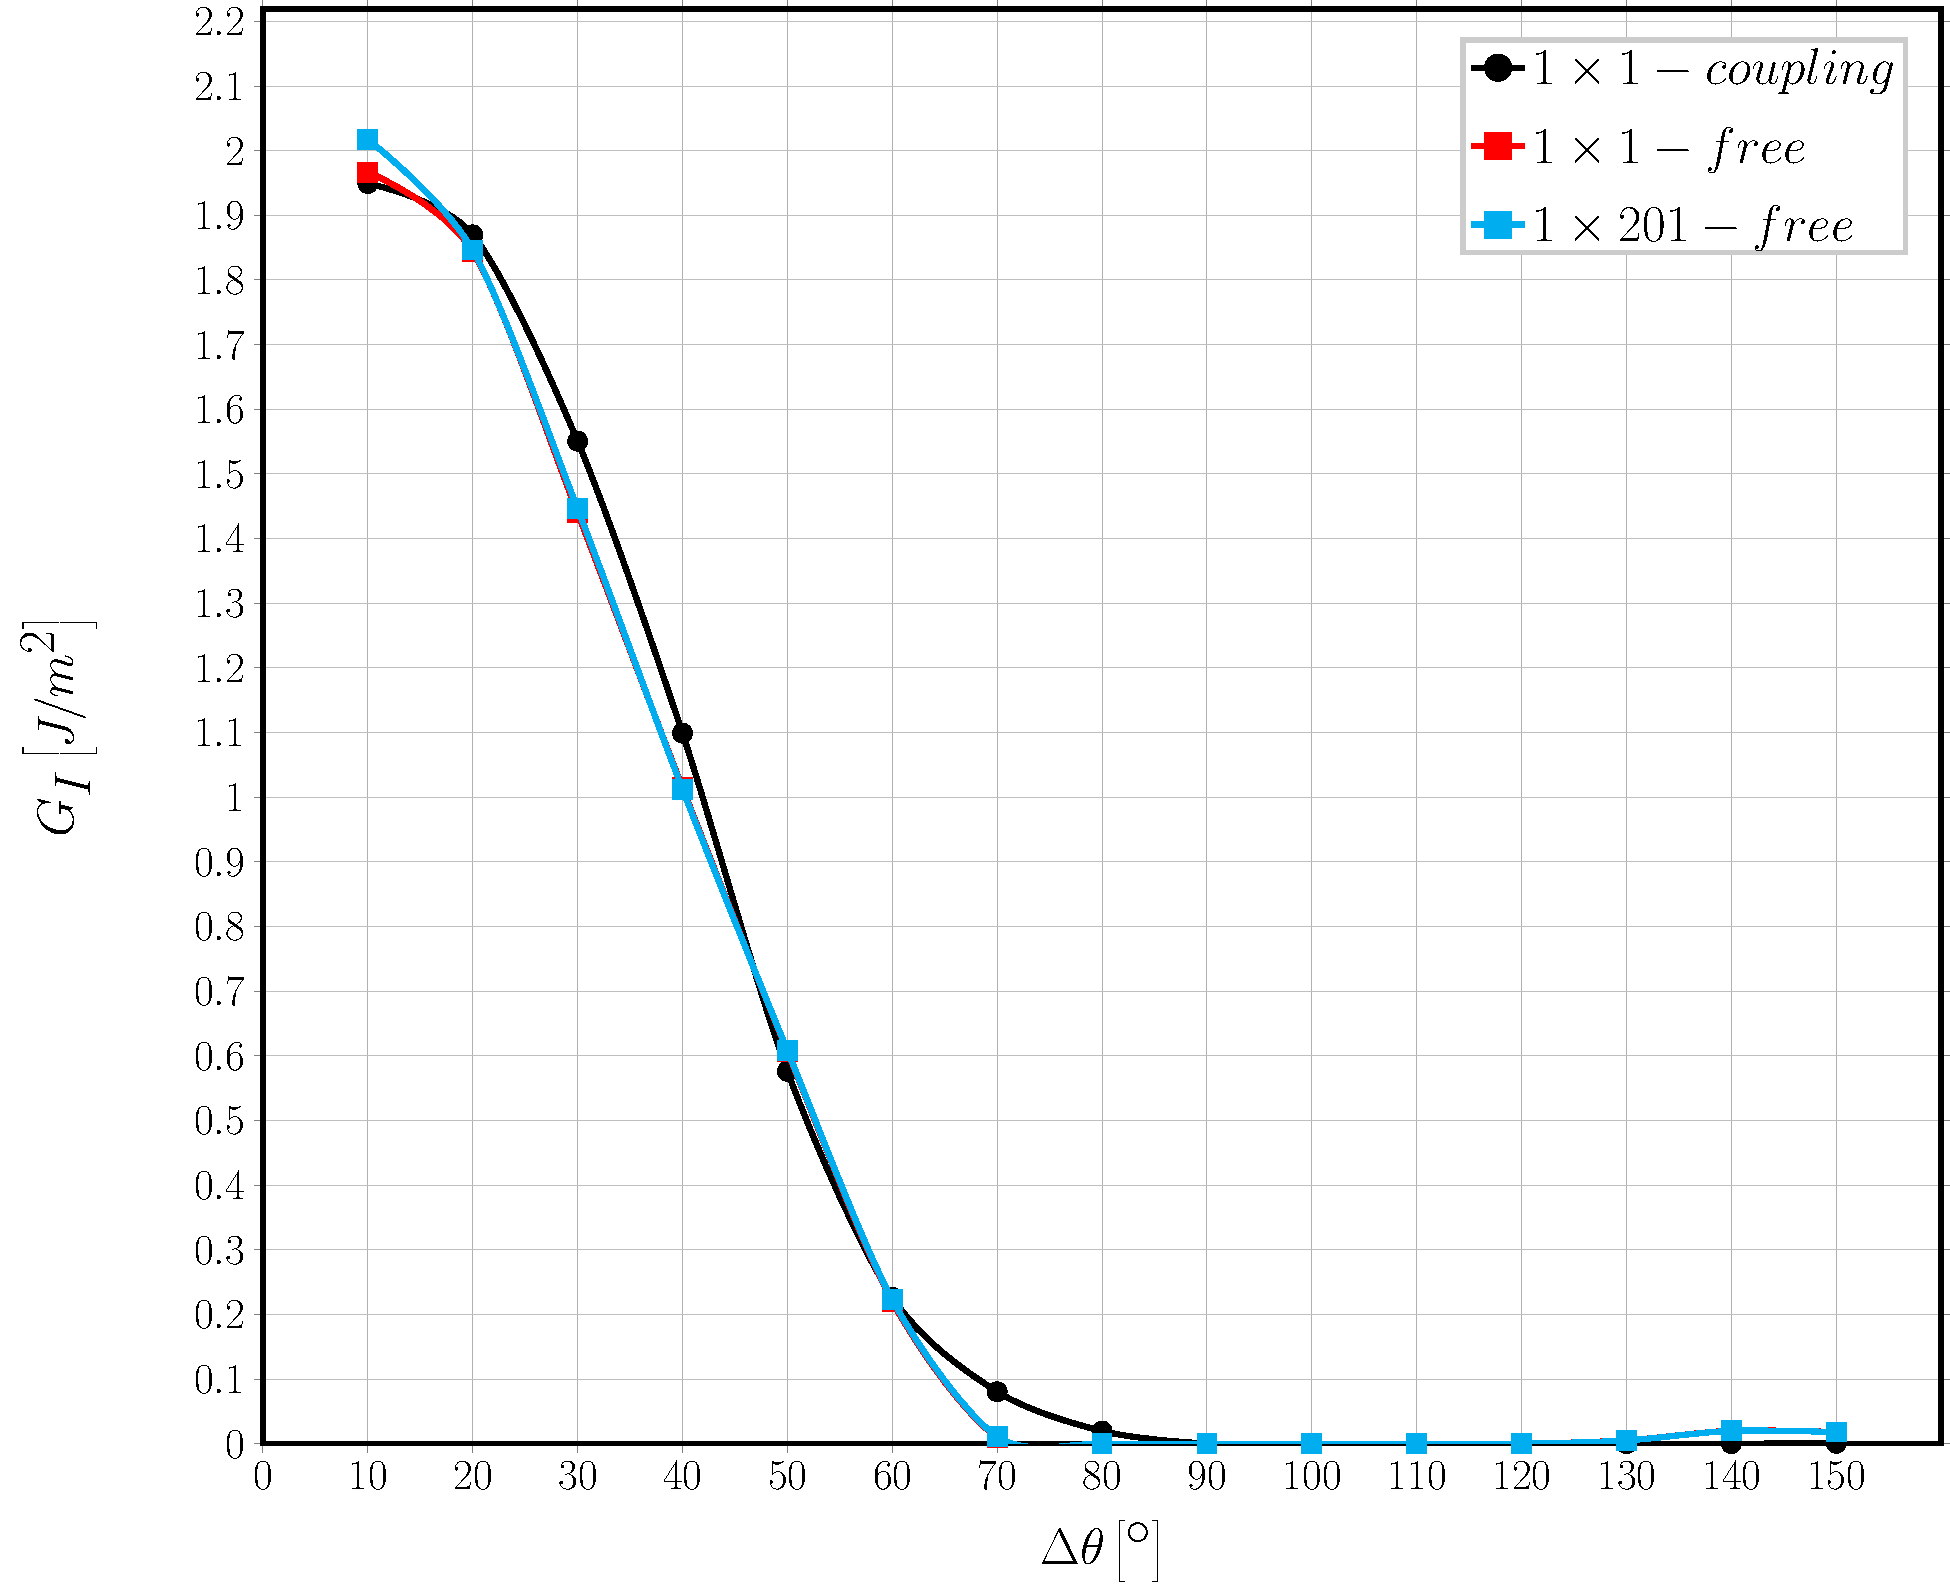
\includegraphics[width=\textwidth]{comparecouplingabovesidefibers-vf60-GI.pdf}
        \caption{$G_{I}$.}\label{subfig:comparisoncoupling60MI}
    \end{subfigure} ~
   \begin{subfigure}[b]{0.475\textwidth}
        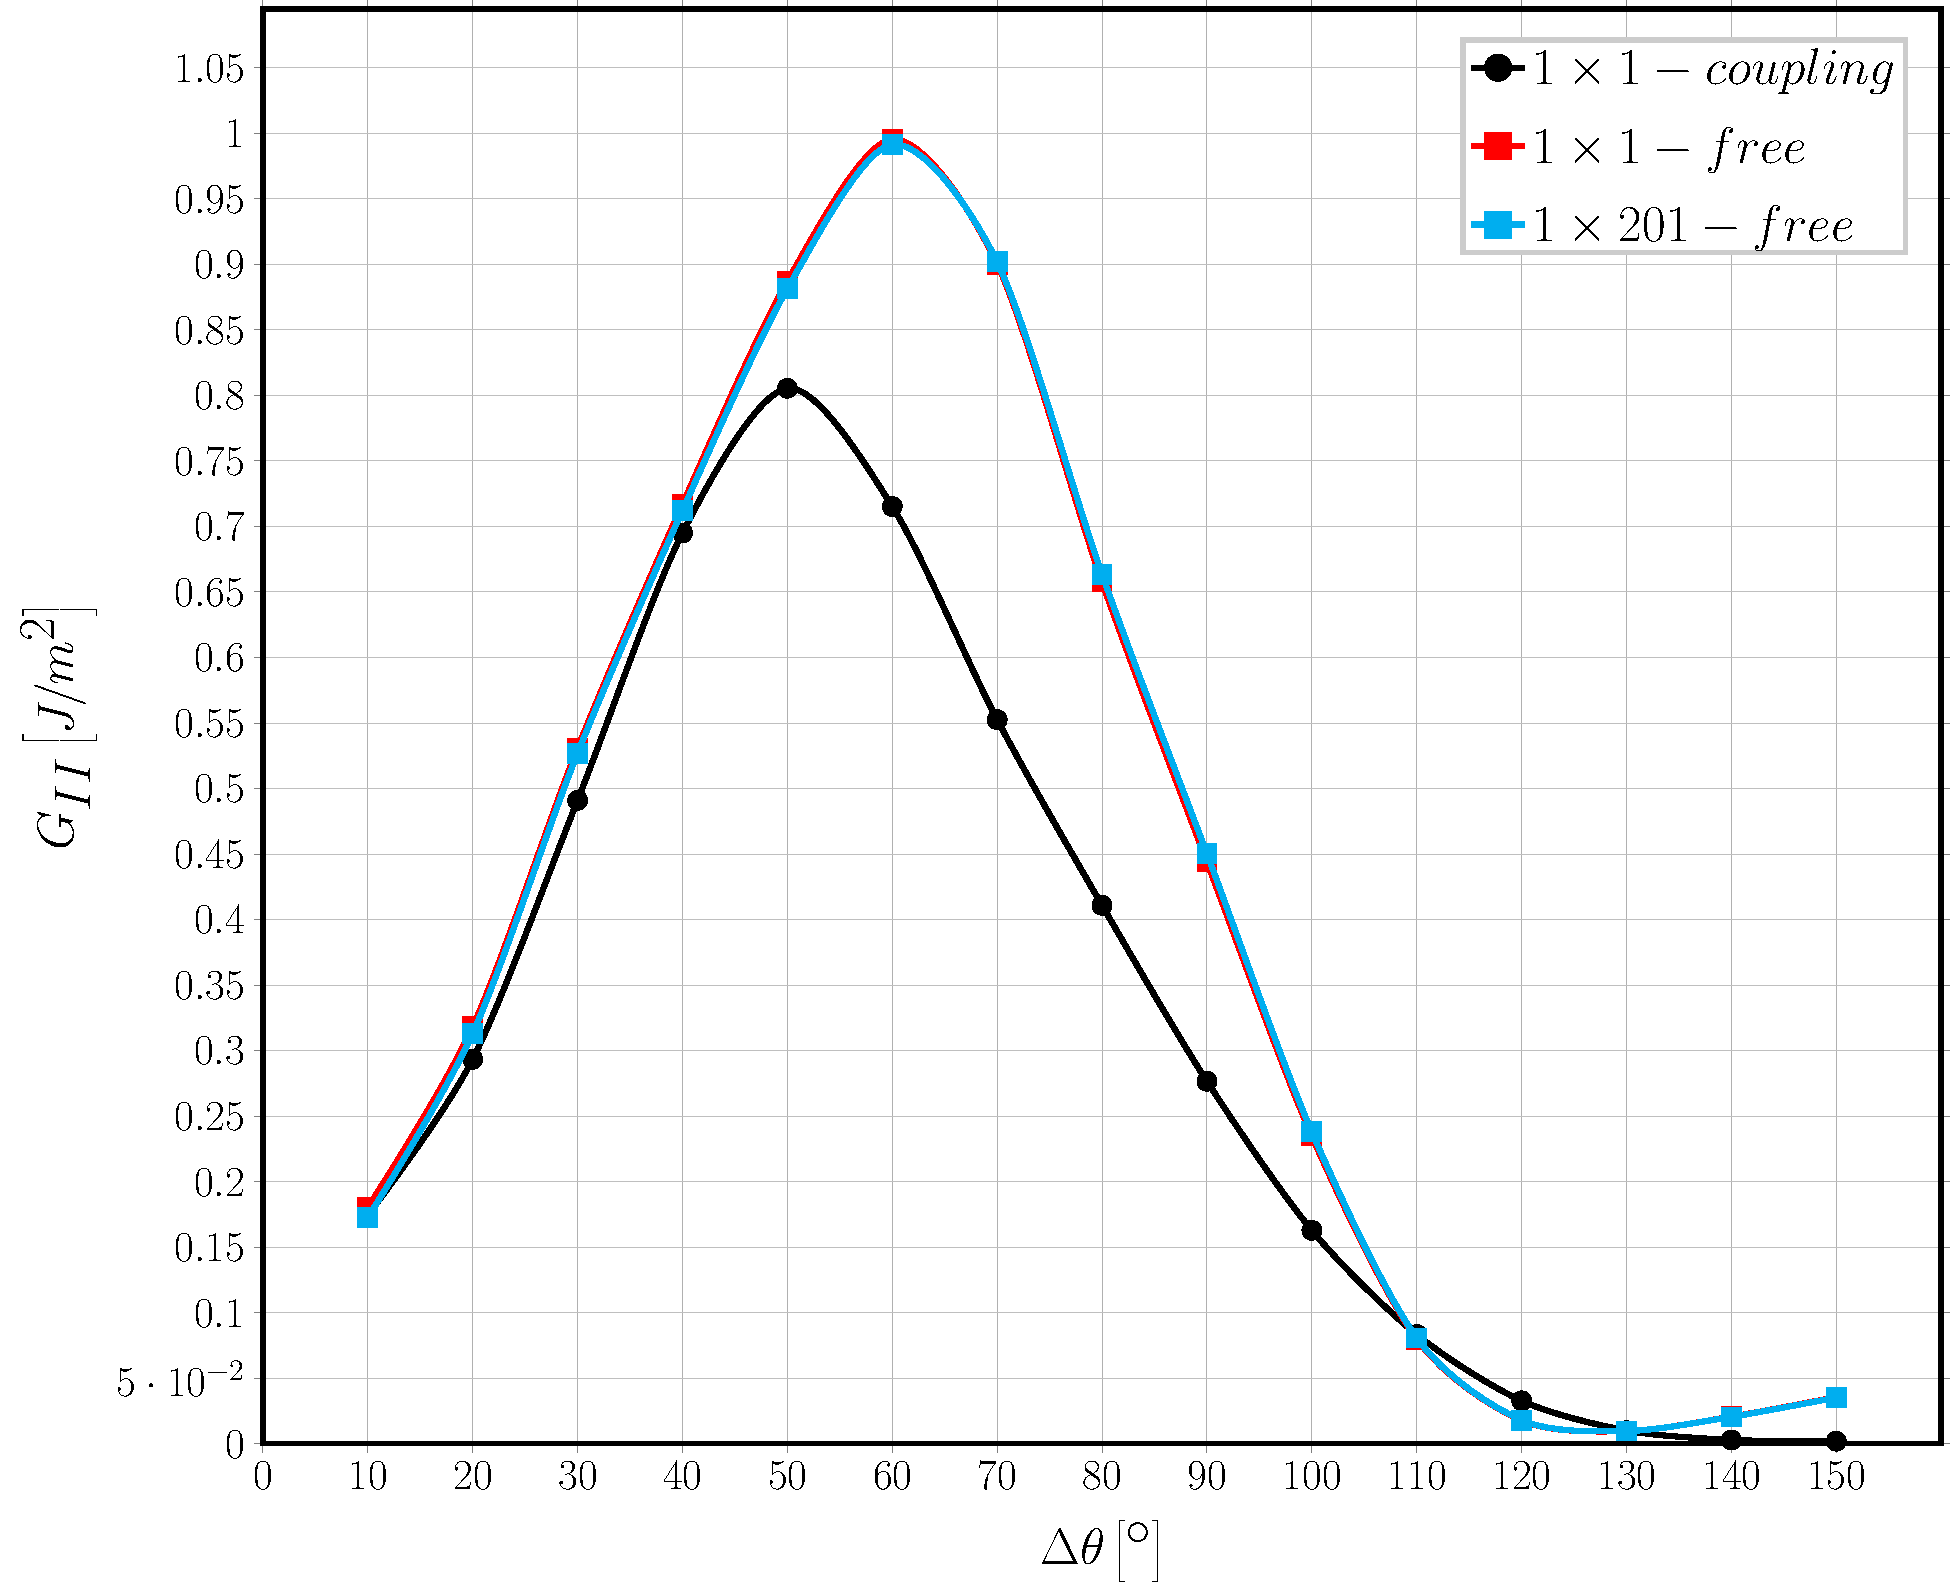
\includegraphics[width=\textwidth]{comparecouplingabovesidefibers-vf60-GII.pdf}
        \caption{$G_{II}$.}\label{subfig:comparisoncoupling60MII}
    \end{subfigure}

\caption{Comparison of the ERR between the single fiber model with coupling conditions along the upper boundary and the multiple fibers model with fibers above. $V_{f}=60\%$ and $\varepsilon_{x}=1\%$.}\label{fig:comparisoncoupling}
\end{figure}

The same comparison for Mode II shows a sizeable difference in the range $50^{\circ}-90^{\circ}$, while the results almost coincide for smaller values of $\Delta\theta$. These observations point to the evidence that debond interaction is more significant in the loading direction than in the transverse one. The lower values of $G_{II}$ of the $1\times 1-coupling$ model in the range $50^{\circ}-90^{\circ}$ are due to the shielding effect of a debond of the same size in the fiber just above the central one (modeled by the coupling boundary condition), which leaves the strip of matrix between the two fibers free to deform away from both of them due to the Poisson’s effect and thus favors Mode I and reduces Mode II. This translates into the lower estimates in Fig.~\ref{subfig:comparisoncoupling60MII} and into the delay in the appearance of the contact zone, particularly evident in Fig.~\ref{subfig:comparisoncoupling60MI}.

\section{Conclusions \& Outlook}

Several models of Repeating Unit Cell, representative of different microstructural arrangements, have been studied in order to investigate the effect on interface crack growth of the presence of debonds and/or fully bonded fibers in the loading and through-the-thickness direction in UD composites. Regular microstructures based on square-packing of fibers have been considered, with debonds appearing at regular intervals measured in terms of fully bonded fibers between them. Local and global fiber volume fractions are everywhere equal to each other by design, which establishes a direct relationship between fiber content and inter-fiber distance. The main conclusions of this work are summarized here in the following.
\begin{enumerate}
\item The presence of a free surface close to the debond causes the effect of the presence of fully bonded fibers along the loading direction to be strongly amplified, leading to higher Mode I and Mode II ERRs and a displacement of the peak $G$ values to larger debonds.
\item The presence of fully bonded fibers in the loading directions causes an increase in ERR, proportional to the number of fully fibers present before the appearance of the closest aligned debond. It seems to exist a characteristic distance between debonds which defines the transition to a non-interactive solution; however, it has not been proved for Mode II in the range of parameters studied.
\item The presence of fibers (fully or partially bonded) in the through-the-thickness direction appears to have a restraining effect on both $G_{I}$ and $G_{II}$, which opposes the magnifying effect of fully bonded fibers placed along the loading direction. Transition to a non-interactive solution is fast, and no change in the solution can be observed by adding more than $2$ fully bonded fibers below and above the central partially debonded one.
\item The presence of a debond in the fiber above the central partially debonded one only delays the appearance of the contact zone, while no significant effect on the ERR can be observed.
\item Increasing the fiber content, which corresponds to a decrease in the inter-fiber distance, magnifies in general the effects described in the previous points.
\item The results and conclusions presented agree strongly with previous observations reported in the literature (~\cite{Sandino2016,Zhuang2018}). A mechanical explanation has been presented based on the mismatch in elastic properties, and particularly Poisson's ratios, and the positions of fibers and debonds with respect to the loading direction. 
\end{enumerate} 

\section*{Acknowledgements}

Luca Di Stasio gratefully acknowledges the support of the European School of Materials (EUSMAT) through the DocMASE Doctoral Programme and the European Commission through the Erasmus Mundus Programme.

\bibliography{refs}

\end{document}
